\documentclass[12pt,a4paper,twoside,openany]{report}
\linespread {1.5}
\setcounter{secnumdepth}{3}

\addtocontents{toc}{\setcounter{tocdepth}{3}} 
\usepackage[a4paper,width=150mm,top=35mm,bottom=30mm,bindingoffset=7mm, outer=1.5cm,inner=2.5cm, hratio=1:1]{geometry}
\addtolength{\footskip}{10pt}
\usepackage{tcolorbox}
\usepackage{float}
\usepackage{enumerate}

\usepackage{fancyhdr}
\pagestyle{fancy} \fancyhf{}
\renewcommand{\sectionmark}[1]{\markright{\it\thesection~ ~#1}}
\renewcommand{\chaptermark}[1]{\markboth{\it Chapter \thechapter}{}}
\fancyhead[RO]{\rightmark} \fancyhead[LE]{\leftmark}
\renewcommand{\headrulewidth}{1pt}
\usepackage[numbers,sort&compress]{natbib}
\usepackage{dcolumn}   
\usepackage{times} 
\usepackage{bm}       
\usepackage{ifpdf}
\usepackage{layout}
\usepackage{titlesec} 
\usepackage{multirow}
\usepackage{dsfont}
\usepackage{booktabs}
\usepackage{threeparttable}
\usepackage{wrapfig}
\usepackage{siunitx}
\usepackage{amssymb,lineno,amsfonts}
\usepackage{graphicx}  
\usepackage{bbm}
\usepackage{mathrsfs}
\usepackage{fancyhdr}
\usepackage{upgreek}
\usepackage{epstopdf}
\usepackage{setspace}
\usepackage[linktocpage=true]{hyperref}
\usepackage[matrix,frame,arrow]{xypic}
\usepackage{float}
\usepackage{amsmath}
\usepackage{natbib}
\usepackage{color} 
\usepackage{subcaption}
\usepackage{emptypage}
\usepackage{pdfpages}
\usepackage{braket}
\usepackage{amsmath}
\usepackage{bbold}
\usepackage{mathtools}
\usepackage{blindtext}
\usepackage{titletoc}
% \usepackage{unicode-math}

\makeindex
\renewcommand*\contentsname{\vspace{-2.5cm} \hspace{12.9cm}\huge{Contents}\\ \HRule \vspace{-2cm}}
\cfoot{\thepage}
\pagenumbering{roman}  

\definecolor{med-blue}{RGB}{25,25,112} 
\hypersetup{colorlinks, linkcolor={blue},citecolor={blue}, urlcolor={blue}}

\newcommand{\outpr}[2]{\vert{#1}\rangle\langle{#2}\vert}
\newcommand{\inpr}[2]{\langle{#1}\vert{#2}\rangle}
\newcommand{\expv}[1]{\langle{#1}\rangle}
\newcommand{\mprod}[3]{\langle{#1}\vert{#2}\vert{#3}\rangle}
\newcommand{\proj}[1]{\outpr{#1}{#1}}
\newcommand{\expec}[1]{\langle{#1}\rangle}
\newcommand{\abs}[1]{\vert{#1}\vert}
\newcommand{\norm}[1]{\vert{#1}\vert^2}
\newcommand{\tr}{\mathrm{Tr}}
\newcommand{\dbydt}{\frac{d}{dt}}
\newcommand{\tabhead}[1]{\textbf{#1}}
\newcommand{\rothead}[1]{\rotatebox{45}{\tabhead{#1}}}
\usepackage{afterpage}
\usepackage{geometry}
\newenvironment{changemargin}[3]{%
	\begin{list}{}{%
			\setlength{\topsep}{0pt}%
			\setlength{\topmargin}{#1}%
			\setlength{\leftmargin}{#2}%
			\setlength{\rightmargin}{#3}%
			\setlength{\listparindent}{\parindent}%
			\setlength{\itemindent}{\parindent}%
			\setlength{\parsep}{\parskip}%
		}%
		\item[]}{\end{list}}
	\newcommand{\HRule}{\vspace{0.2cm}\rule[20pt]{\linewidth}{0.50mm}}

\begin{document}

\begin{titlepage}
\begin{center}

\vspace*{1cm}

\Huge
\textbf{The Dynamics and Statistics of Public Opinion}

\vspace{0.5cm}
\LARGE


\vspace{1.5cm}

\textbf{Ritam Pal}

\vfill

A thesis submitted in partial fulfillment of the requirements for the degree of\\
Doctor of Philosophy in Physics

\vspace{0.8cm}


\Large
Department of Physics\\
Indian Institute of Science Education and Research\\
Pune\\
India

\vspace{0.8cm}

\Large
\today

\end{center}
\end{titlepage}

\newpage

\chapter*{Abstract}
\addcontentsline{toc}{chapter}{Abstract}

This thesis navigates the complex landscape of human collective behavior, from opinion formation in online social networks to the competitive dynamics of democratic elections. We first address the pervasive issue of opinion polarization by introducing and optimizing a "random nudge" intervention, demonstrating its efficacy in fostering depolarization without inducing radicalization. Shifting focus to democratic elections, we undertake a comprehensive data-driven analysis spanning 34 countries and multiple decades, revealing the critical role of voter turnout in shaping electoral statistics. 

We unveil a novel, robust universality in the scaled distribution of margin-to-turnout ratios, validated across diverse electoral scales. To explain this, we develop the Random Voting Model (RVM), a parameter-free framework that remarkably predicts not only this universality but also the distributions of winner/runner-up vote shares and overall margins, driven solely by voter turnout data. The RVM's predictive power is rigorously tested against extensive Indian election data, showcasing its accuracy from parliamentary constituencies down to individual polling booths and revealing a characteristic scale-invariance in Indian margin distributions. 

Finally, we demonstrate the practical applications of our findings: the random nudge as an intervention tool for reducing polarization and the RVM as a statistical framework for detecting potential electoral malpractices. This work underscores the profound insights gained by applying statistical physics principles to understand and potentially shape complex societal phenomena.

\newpage

\chapter*{Synopsis}
\addcontentsline{toc}{chapter}{Synopsis}


This thesis is a journey that starts by acknowledging the messy, complex world of human opinions and decisions. It then zooms into a specific problem in the digital age (polarization) and proposes a clever, non-intrusive solution. From there, it broadens its gaze to one of the most significant forms of collective decision-making – elections – embarking on a quest for hidden order. This quest leads to the development of a deceptively simple yet powerful model (the RVM) that not only explains observed universalities but also offers tools to predict electoral behavior and safeguard democratic processes. The common thread? The surprising power of statistical thinking and the unexpected elegance that emerges when we embrace randomness.

\section*{Chapter Summaries}

\subsection*{Chapter 1: A Physicist's Map of Human Opinions}

Chapter 1 establishes the foundation for investigating human collective behavior through the lens of statistical physics. It positions society as a complex system where numerous interacting individuals generate emergent behaviors across multiple scales. The chapter introduces two primary domains of investigation—opinion formation in digital networks and electoral patterns in democratic systems—and explains their shared conceptual foundations despite apparent differences. It argues that opinions do not exist as static properties but as dynamic outcomes of social interactions, increasingly mediated by digital technologies that reshape information diffusion processes. The chapter reviews how traditional opinion dynamics models (voter model, Sznajd model) typically predict consensus, while empirical evidence shows bimodal distributions and polarization, especially on controversial issues. Advanced models incorporating homophily and algorithmic effects can now reproduce the emergence of polarized states and echo chambers. The chapter also discusses the value of statistical physics approaches to elections, where previous attempts at finding universality have yielded limited results despite extensive data availability. The chapter concludes by outlining the thesis structure, previewing how it will apply statistical physics tools to understand both opinion polarization and electoral statistics, with randomness serving as both explanatory principle and intervention tool.

\subsection*{Chapter 2: A Light Nudge Against Online Polarization}

Chapter 2 addresses the problem of opinion polarization in digital environments through a novel intervention strategy. Building on an empirically calibrated opinion dynamics model that incorporates homophily—the tendency to interact with similar others—the chapter demonstrates how polarization emerges through reinforced echo chambers in online social networks. The model features $N$ agents with continuous opinions $x_i$ whose evolution is governed by activity-driven dynamics and homophilic interactions. When homophily is strong, the system naturally segregates into distinct opinion clusters. The chapter introduces the "random nudge" intervention: with probability $p$, active agents interact randomly rather than according to homophilic preferences. Comprehensive simulations with $N=5000$ agents show that even a small nudge probability ($p=0.01$) significantly reduces polarization across multiple metrics: the distance between mean positive and negative opinions ($\bar{\Delta}$), the distance between peaks in bimodal distributions ($\Delta_{peak}$), and the standard deviation of opinions ($\sigma$). Network analysis reveals the intervention transforms the interaction structure from segregated clusters to a well-mixed network, effectively disrupting echo chambers. However, higher nudge probabilities can lead to undesirable radicalization, where all agents adopt the same extreme position. The chapter presents an optimization framework that balances depolarization against radicalization risk, demonstrating that the optimal nudge follows a power-law relationship $p \cdot f^A = B$, where $f$ is the fraction of the population nudged. This mathematically optimized approach offers a non-invasive intervention that requires no interpretation of specific opinions, making it both privacy-preserving and practically implementable in recommendation systems.

\subsection*{Chapter 3: Digging into the Data: The Foundation of Electoral Analysis}

Chapter 3 builds the empirical foundation for electoral analysis through comprehensive data collection and preparation. The chapter details the extensive effort to compile election data from 34 countries across six continents using sources such as the Constituency-Level Election Archive, national election commission websites, and the MIT Election Data and Science Lab. The dataset features key variables including voter turnout ($T$), candidate vote shares, margins of victory ($M$), and constituency identifiers. A distinctive feature of the data collection is its multi-scale approach, particularly evident in the Indian election data, which spans from polling booth level (${\sim}10^2$ voters) to assembly constituencies (${\sim}10^5$ voters) to parliamentary constituencies (${\sim}10^6$ voters). The chapter outlines the significant data cleaning challenges encountered: handling missing values, standardizing inconsistent formats, resolving encoding issues especially for non-Latin scripts, and addressing boundary redistricting problems in longitudinal data. To ensure statistical robustness, strict filtering criteria were applied, including a minimum threshold of 400 data points per country. The chapter presents comprehensive summary statistics highlighting the diversity of electoral patterns across democratic systems, with mean turnout rates ranging from approximately 45\% to 90\% and significant variation in margins of victory between established and emerging democracies. This meticulously prepared dataset, emphasizing quality over mere quantity, provides the essential empirical backbone for the subsequent analyses of universal patterns in electoral behavior.

\subsection*{Chapter 4: Universal Clues in the Ballot Box}

Chapter 4 presents a breakthrough discovery of universal patterns in electoral statistics across diverse democratic systems. The chapter begins by examining traditional electoral variables—turnout ($T$) and margin of victory ($M$)—noting that raw turnout distributions $g(T)$ vary dramatically across countries in both shape and support, while scaled margin distributions $f(M/\langle M \rangle)$ show certain similarities but also notable differences, particularly in their decay patterns. Analysis across different electoral scales confirms that these distributions remain scale-dependent, with turnouts at polling booth level differing by orders of magnitude from constituency level. The chapter introduces a crucial innovation: the specific margin $\mu = M/T$, representing the margin normalized by the local turnout. When further scaled to $x = \mu/\langle\mu\rangle$, a remarkable universality emerges. The distribution $F(x)$ of this scaled specific margin collapses onto a single universal curve across 32 countries, despite vast differences in their electoral systems, cultural contexts, and historical backgrounds. This universality transcends both country-specific details and scale effects, suggesting a fundamental statistical signature intrinsic to competitive democratic processes. The chapter concludes by deriving an analytical expression for the universal distribution, $P(\mu) = \frac{(1 - \mu)(5 + 7\mu)}{(1 + \mu)^2(1 + 2\mu)^2}$, preparing the ground for a theoretical model that explains this empirical universality from first principles.

\subsection*{Chapter 5: The Random Voting Model: When Chance Explains Choice}

Chapter 5 develops the Random Voting Model (RVM), a parameter-free theoretical framework that explains the universal patterns discovered in electoral statistics. The RVM represents electoral competition through a minimal statistical framework where candidates are assigned random weights $w_{ij} \sim \mathcal{U}(0,1)$, which are normalized to probabilities $p_{ij} = \frac{w_{ij}}{\sum_{k=1}^{n^c_i} w_{ik}}$. Despite its simplicity, the RVM provides analytical derivations for the universal scaled specific margin distribution observed empirically. Using order statistics, the chapter derives the probability density function $P(\mu) = \frac{(1 - \mu)(5 + 7\mu)}{(1 + \mu)^2(1 + 2\mu)^2}$ for the specific margin, which leads to the universal distribution $F(x) = \langle \mu \rangle P(x\langle \mu \rangle)$ for the scaled specific margin. The model establishes a crucial insight: the distribution of margins $Q(M)$ is fundamentally driven by the distribution of turnouts $g(T)$. The chapter demonstrates this by deriving analytical expressions for margin distributions corresponding to different turnout distributions (exponential, power law, Gaussian, uniform) and showing that the tails of margin distributions mimic the corresponding turnout distributions. For exponential turnout $g(T) \propto e^{-T/\tau}$, the margin distribution has asymptotic behavior $Q(M) \propto \frac{\tau}{3M^2}e^{-M/\tau}$; for power law turnout $g(T) \propto T^{-\alpha}$, the margin distribution also follows a power law with the same exponent. The chapter extends the model by introducing the concept of "effective number of candidates" $(^{(E)}n^c)$ to account for different electoral scales. This allows application of different variants—RVM$(T,2)$ or RVM$(T,3)$—depending on the electoral scale. The chapter validates the model using Indian election data across multiple scales (polling booth to parliamentary constituency), demonstrating remarkable agreement between theoretical predictions and empirical distributions for winner votes, runner-up votes, and margins. A unique scale invariance is discovered in Indian margin distributions, where scaled distributions collapse onto a single curve across vastly different electoral scales, a feature absent in other countries like the USA. This comprehensive validation establishes the RVM as a powerful predictive framework for electoral statistics driven solely by turnout distributions.

\subsection*{Chapter 6: From Theory to Practice: Applications and Interventions}

Chapter 6 translates theoretical insights into practical applications that address two critical challenges facing modern democracies: opinion polarization and electoral integrity. The first application details the implementation of the "random nudge" as an algorithmic intervention in social media recommendation systems. By modifying interaction probabilities as $\widetilde{P}_{ij} = p \times \frac{1}{N - 1} + (1 - p) \times P_{ij}$, the intervention introduces controlled randomness into opinion formation processes. The chapter presents an optimization framework that balances depolarization against radicalization risk, showing that polarization decreases as a stretched exponential function $\exp(-p^\gamma)$ of the nudge strength, with $\gamma \approx 0.3$. Network analysis demonstrates how the intervention disrupts echo chamber formation by preventing network segregation into distinct opinion clusters. The chapter discusses practical implementation details, ethical considerations, and limitations of this approach. The second application develops the RVM as a diagnostic tool for electoral integrity. By establishing statistical baselines for what fair competitive electoral processes should produce, the model enables detection of anomalies that may indicate irregularities. The chapter presents case studies of Ethiopia and Belarus, where significant deviations from the universal pattern align with independent assessments of electoral concerns. The RVM diagnostic approach offers standardized metrics for cross-national comparison, temporal tracking of electoral competition, and early warning of emerging integrity issues. The chapter concludes by outlining implementation pathways for both applications, emphasizing the need for multidisciplinary collaboration, controlled trials, and integration with existing frameworks for polarization reduction and election monitoring.

\subsection*{Chapter 7: Looking Forward: Randomness, Democracy, and Beyond}

Chapter 7 synthesizes the key findings from our research and explores their broader implications. It highlights how randomness serves as both an explanatory principle and a constructive force in complex social systems. In the context of opinion dynamics, our research demonstrated how a small "random nudge" probability ($p = 0.01$) can successfully disrupt echo chambers and foster depolarization without compromising user privacy or platform functionality. In electoral analysis, our Random Voting Model revealed how the inherently stochastic nature of voting processes generates robust universal patterns across vastly different electoral systems, with the scaled distribution of margin-to-turnout ratios $F(x)$ showing remarkable universality across 32 democratic nations. The chapter details key methodological contributions including the critical importance of variable selection in uncovering universal patterns, the value of multi-scale analysis across different electoral hierarchies, and the efficacy of minimalist models in capturing essential system properties. It discusses theoretical advances such as the derivation of analytical expressions for electoral statistics as functions of turnout distribution and the demonstration that complex political phenomena can be governed by relatively simple statistical laws. The chapter acknowledges limitations and open questions, including the boundaries of the observed universality, the need for dynamic models capturing temporal evolution, and the role of strategic behavior in shaping statistical patterns. It outlines promising directions for future research, including extension to other competitive domains, development of dynamic models incorporating feedback mechanisms, and optimization frameworks for intervention design. The chapter concludes by reflecting on the ultimate goal of contributing to healthier information ecosystems and more robust democratic processes through principled analysis and thoughtful intervention.

\section*{Key Contributions}

\begin{itemize}
\item Development of a random nudge intervention for reducing opinion polarization in social networks
\item Discovery of universal patterns in electoral competition across 34 countries
\item Creation of the Random Voting Model (RVM) as a parameter-free framework for predicting electoral statistics
\item Demonstration of scale-invariant behavior in Indian electoral data
\item Practical applications for both social media intervention and electoral integrity monitoring
\end{itemize}

\section*{Methodological Innovations}

\begin{itemize}
\item Strategic use of randomness as a constructive force in complex systems
\item Order statistics and scaling analysis for social system modeling
\item Data-driven approaches to uncovering universal patterns in social phenomena
\item Cross-scale validation from polling booths to national constituencies
\end{itemize} 

\linespread {1}
\cleardoublepage
\tableofcontents
\cleardoublepage
\titlespacing*{\chapter}{0pt}{-20pt}{20pt}

\titleformat{\chapter}[display]
{\bfseries\Large}
{\filright\MakeUppercase{\chaptertitlename} \Large\thechapter}
{1ex}
{\vspace{-0.5cm} \HRule \vspace{-0.5cm} \filleft}
[\HRule]
\pagestyle{fancy}
\setcounter{page}{1}
\pagenumbering{arabic}
\cleardoublepage

\chapter{A Physicist's Map of Human Opinions}
\label{chap1}
Society represents one of nature's most intricate complex systems—a vast ensemble of interacting individuals whose collective behaviors emerge across multiple scales, from ephemeral digital trends to enduring democratic institutions. The emergent properties arising from these interactions often manifest as non-trivial macroscopic patterns that cannot be easily inferred from individual behaviors \cite{galam2012sociophysics}. Much like how individual water molecules give rise to the unexpected phenomenon of waves, individual human decisions combine to create societal patterns that no single interaction could predict. This thesis employs the tools of statistical physics to investigate two fundamental aspects of collective human behavior: opinion formation in digital networks and universal patterns in democratic elections. Through this examination, we demonstrate that randomness, properly understood and harnessed, serves as both an explanatory principle and a constructive force for understanding and improving social systems.

\section{Society as a Multi-Scale Complex System}
Human society operates across extraordinarily diverse scales, both spatial and temporal. Spatially, interactions span from local communities to global networks, encompassing physical proximity interactions and increasingly, technology-mediated connections that transcend geographic constraints \cite{social-media-as-public-opinion}. Temporally, processes range from millisecond-scale information transmission to decade-spanning political movements and generational cultural shifts. This multi-scale nature creates layered feedback mechanisms that make social systems resistant to reductionist analysis.

Consider how a single tweet can trigger cascading reactions across millions of users within minutes, while simultaneously contributing to slowly-evolving cultural narratives that unfold over years. These cross-scale interactions create feedback loops where macro-level structures shape individual behaviors, which in turn reshape those very structures—a dynamic reminiscent of how atoms collectively determine the properties of materials which then constrain atomic movement.

Within this complex landscape, opinion formation and electoral processes represent critical mechanisms through which individuals collectively navigate their shared environment. These processes share common features with physical systems that have long been studied using statistical mechanics—they involve numerous interacting components, exhibit emergent behaviors, and often display robust statistical regularities despite their apparent complexity \cite{galam1982sociophysics, galam1991towards}. However, they also present unique challenges: human agents possess agency, adaptability, and strategic behavior absent in physical particles.

The statistical physics approach to social dynamics leverages powerful analytical tools developed for understanding physical systems while acknowledging these distinctive features of social interactions. This approach focuses not on predicting individual behavior but on identifying statistical patterns that emerge at the population level, along with the mechanisms that generate them. The value of such an approach lies in its ability to abstract away unnecessary details while preserving essential dynamics that govern system behavior.

\section{Opinion Formation: Emergent Patterns of Social Interaction}
Opinions do not exist as static, independent properties of individuals but rather as dynamic outcomes of complex social interactions. These interactions are increasingly mediated by digital technologies that reshape the fundamental processes of information diffusion and opinion formation \cite{social-media-as-public-opinion}. Online platforms now serve as primary arenas where individuals encounter information, form judgments, and express beliefs on topics ranging from trivial consumer choices to consequential political positions.

Much as stars form nebulae through their gravitational pull on surrounding matter, influential voices and trending topics create opinion clusters that shape the broader information landscape. These nebulae of opinion are not fixed—they expand, contract, split, and merge as new information enters the system and social connections evolve.

The information revolution has lowered the entry barrier for nearly everyone to participate and contribute to shaping opinions and policies on various issues. This has been largely aided by the easy availability of social media infrastructure through mobile devices. Increasingly, the collective opinions expressed through various social media platforms are thought to be one barometer of the public mood on any contentious issue of the day \cite{social-media-as-public-opinion}. This provides an interesting testing ground for the dynamics and statistical physics of interacting multi-agent systems since the online nature of interactions provides fine-grained data for quantitative analysis and comparison with model results.

Recent empirical studies have documented concerning trends in these digital opinion landscapes. Controversial issues consistently display bimodal opinion distributions, indicating polarization rather than consensus \cite{biased-assimilation-and-attitude-polarization, have-americans-social-attitudes-become-more-polarized, paritisans-without-constrait-political-polarization-and-trends}. This polarization is often reinforced through homophilic interactions—individuals preferentially engaging with others holding similar views—creating what researchers term ``echo chambers" \cite{echo-chambers-online, echo-chambers-emotional-contagion-and-group-polarization-on-facebook, quantifying-echo-chamber-effects-in-information-spreading-over-political-communication, political-discourse-on-social-media-echo-chambers, The-echo-chamber–effect-on-social-media}. Platform recommendation algorithms, optimized for user engagement, frequently amplify these natural homophilic tendencies, potentially accelerating polarization processes \cite{link-recommendation-algorithms-and-dynamics-of-polarization-in-social-networks}.

\subsection{Models of Opinion Dynamics and Polarization}
The study of opinion formation and its dynamics has attracted researchers for decades. The analysis of opinion dynamics from the statistical physics perspective can be traced back to the work of DeGroot \cite{reaching-a-consensus}, which provides a framework for reaching a consensus. Several models, including the voter model \cite{the-voter-model, reality-inspired-voter-models-a-mini-review}, Sznajd model \cite{opinion-evolution-in-closed-community, sznajd-review}, and their variants which have a strong basis in a framework of interacting spins, suggest that large participatory interactions among agents might also lead to the emergence of consensus.

At their core, these models capture a fundamental insight: opinions change through social influence. When individuals interact, their views tend to shift based on those they encounter—much like how particles exchange energy upon collision. The simplest models assume a straightforward convergence process, where repeated interactions lead to a gradual alignment of views across the population.

However, empirical results have shown that the distribution of opinions tends to show a bimodal distribution pattern corresponding to polarization, especially on controversial issues of the day \cite{biased-assimilation-and-attitude-polarization, have-americans-social-attitudes-become-more-polarized, paritisans-without-constrait-political-polarization-and-trends}. Culture dissemination model \cite{the-dissemination-of-culture}, one of the first higher-dimensional modeling approaches to opinion dynamics, which also incorporates the human tendency to interact with similar persons, shows that despite there being local convergence, global polarization can be reached. 

Other discrete models by Galam et al. \cite{galam1982sociophysics, galam1991towards, galam2002minority, galam2012sociophysics} explain the effects of consensus, attitude changes in groups, and the spreading of minority opinions. In the presence of stubborn agents, these models can also capture the effect of polarization \cite{galam2007role, galam2016stubbornness, galam2011collective}. Different variants of the bounded confidence model \cite{mixing-beliefs-among-interacting-agents, opinioin-dynamics-and-bounded-confidence} can also capture many empirically found trends in the distribution of opinions. These models can reproduce consensus, bimodal, or multi-modal opinion distributions depending on the confidence interval.

More recent models have incorporated homophily and algorithmic feedback effects, successfully reproducing the emergence of polarized states and echo chambers. Among these, the model by Baumann et al. \cite{modeling-echo-chambers-and-polarizaiton-dynamics-in-social-networks} demonstrates particular empirical fidelity, capturing key features of digital polarization including active extremists, opinion clusters, and reinforcement mechanisms.

Traditional opinion dynamics models from statistical physics typically predict convergence toward consensus under broad conditions. These models fail to capture the persistent polarization observed empirically. Recent empirical evidence for echo chamber effects has been reported from several social media platforms \cite{echo-chambers-emotional-contagion-and-group-polarization-on-facebook, quantifying-echo-chamber-effects-in-information-spreading-over-political-communication, political-discourse-on-social-media-echo-chambers, The-echo-chamber–effect-on-social-media}. Few recent opinion dynamics models \cite{modeling-echo-chambers-and-polarizaiton-dynamics-in-social-networks, polarized-idoelogy, link-recommendation-algorithms-and-dynamics-of-polarization-in-social-networks, social-influence-and-unfollowing-accelerate-the-emergence-of-echo-chambers} have qualitatively captured the features of echo chambers, which have been shown to arise from personalized interactions among peers in an online setting, which might be accelerated through the platform's recommendation engine.

\subsection{Addressing Polarization and Echo Chambers}
Though having diverse opinions might be a desired outcome, extreme polarization leads to network segregation \cite{segregatioin-and-clustering}, which often bottlenecks the information flow in social networks. At an individual level, people in highly polarized environments experience reduced exposure to diverse perspectives, and at a societal level, this fragmentation can undermine the shared factual basis necessary for collective decision-making.

Echo chambers, often linked to polarization, are known to be responsible for sustaining misinformation for a longer time on social networks \cite{echo-chambers-and-viral-misinformation, the-spreading-of-misinformation-online}. Think of echo chambers as information cul-de-sacs, where ideas circulate but rarely exit—creating closed loops that resist correction or evolution. As individuals become increasingly isolated in these self-reinforcing information environments, their resistance to contradictory information grows, making depolarization increasingly difficult.

These problems call for intervention mechanisms, which should be safe and non-invasive. Just as a physicist might introduce a controlled perturbation to study or alter a physical system's behavior, we can consider strategic interventions in digital networks to reduce harmful polarization without compromising individual agency.

It might appear that in the case of controversial topics, the interaction and debate will always lead to polarized states of opinion. But the underlying mechanism for polarization—the reinforcement of opinions through interaction between like-minded people—leaves us wondering if any intervention will help to reconcile disparate opinions.

Understanding and potentially mitigating digital polarization presents both theoretical and practical challenges. Any intervention must balance multiple objectives: reducing polarization without promoting radicalization, preserving user engagement, and respecting individual privacy. Additionally, defining a ``healthy" opinion distribution is itself normatively complex, requiring careful consideration of democratic values and information ecosystem diversity.

Echo chambers are increasingly becoming more apparent in online social media platforms. A generic tendency to interact with people who hold similar opinions as ours can lead to echo chambers, and this effect is, in turn, amplified by the recommendation engines on social media platforms. These algorithmically driven engines recommend similar connections or content in order to keep the users of those platforms engaged.

\section{Electoral Processes: Critical Events in Collective Decision-Making}
Electoral processes represent a formalized mechanism through which individual preferences aggregate to produce collective decisions. If everyday opinion formation resembles the slow accretion of nebulae, elections are like supernovae—intense, concentrated events where the energy of millions of individual choices release their power in a single moment, potentially altering the landscape of governance.

Elections, the cornerstone of democratic societies, are usually regarded as unpredictable due to the complex interactions that shape them at different levels. Democratic elections constitute some of the most extensively documented instances of large-scale collective human behavior, with records spanning decades and encompassing hundreds of millions of voters.

One of the cornerstones of democratic societies is that governance must be based on an expression of the collective will of the citizens. The institution of elections is central to the operational success of this system. Elections to public offices are the best-documented instances of collective decision-making by humans, whose outcome is determined by multiple agents interacting over a range of spatial and temporal scales. These features make elections an interesting test-bed for statistical physics whose key lesson is that a multitude of complex interactions between microscopic units of a system can manifest into robust, {\it universal} behavior at a macroscopic level \cite{anderson1972more,strogatz2022fifty,CasForLor2009, JedSzn2019, MigTor2020, galam2012, brams2008, ForMacRed2013, Bouchaud2023, SenCha2014, PerJorRan2017,JusHolKan2022,redner2019reality}. A collection of gas molecules or spins are examples that display such emergent macroscopic features \cite{REI65}, and so are complex processes such as earthquakes \cite{Corral2004,Corral2006} and financial markets \cite{PleGopRos1999}. In the context of elections, such universal behaviors serve to distill the complexities of electoral dynamics into understandable and predictive frameworks and safeguard its integrity. 

\subsection{The Search for Universal Patterns in Electoral Data}
Unsurprisingly, the possibility of universality in elections attracts significant research attention \cite{CosAlmAnd1999, ForCas2007, BorBou2010, mantovani2011scaling, BokSzaVat2018, ChaMitFor2013, hosel2019universality}. Several works have studied and proposed models for ({\it a}) the distribution $q(\sigma)$ of the fraction of votes $\sigma$ obtained by candidates (or the vote share), and ({\it b}) distribution $g(\tau)$ of voter turnout $\tau$. While $\sigma$ is indicative of popularity, $\tau$ indicates the scale of the election. Though some universality has been observed in $q(\sigma)$ or $g(\tau)$ within a single country \cite{ForCas2007,CosAlmAnd1999, BorBou2010} or in countries with similar election protocols \cite{ForCas2007, ChaMitFor2013}, deviations from claimed universalities have also been reported \cite{ChaMitFor2013, Kon2017,Kon2019, CalCroAnt2015, BorRayBou2012} due to variations in the size (scale) of electoral districts and weak party associations. 

Though voting patterns tend to display spatial correlations \cite{FerSucRam2014, BraDeA2017,MicIlkAtt2021,MorHisNak2019}, it is not known to be universal. Despite the availability of enormous election data and persistent attempts, a robust and universal emergent behavior, valid across different scales and countries with vastly different election protocols, is yet to be demonstrated. This absence of truly robust universality across different countries and electoral scales has remained a significant gap in our understanding of collective voting behavior.

\subsection{Margins of Victory and Voter Turnout}
Among the many statistics of interest, the \emph{margin} of victory, defined as the difference between votes for the winner and runner-up candidates, encodes key information about the competitiveness of elections. While margins of victory have been previously studied \cite{jacobson1987marginals, mccann1997threatening, mulligan2003empirical, magrino2011computing, xia2012computing, bhattacharyya2021predicting}, often independently of voter turnouts. 

However, our empirical analysis using extensive election data \cite{india_data, clea, canada_data, DVN/VOQCHQ_2018} from 34 countries (from 6 continents) spanning multiple decades and electorate scales, shows that margins of victory are strongly correlated with voter turnout and can be leveraged to demonstrate a robust universality. By examining how these quantities scale with each other, we uncover patterns analogous to scaling laws in physical systems—where relationships between variables remain consistent across different scales of observation.

The significance of such findings extends beyond academic interest. Understanding the statistical properties of electoral competition can provide baselines for detecting anomalies that might indicate manipulation \cite{brigaldino2011elections, frear2014parliamentary, belarus_report, czwolek2021belarusian, bedford_2021, klimek2012statistical, jimenez2017testing} inform electoral system design, and shed light on the fundamental nature of democratic competitions.

\section{Structural Overview and Research Framework}

The thesis proceeds through several interlinked investigations, each reinforcing a unified theme: leveraging randomness constructively to decode and enhance social systems:

\textbf{Chapter 2} introduces and optimizes the ``random nudge" intervention strategy against digital polarization. Building on our understanding of opinion dynamics, we demonstrate how carefully calibrated random interventions can counteract the reinforcement mechanisms that drive polarization without compromising system integrity.

\textbf{Chapter 3} details extensive data collection and curation efforts, laying the empirical foundation for electoral analysis. This chapter bridges theory with real-world observation, establishing the robust dataset necessary for testing universal patterns.

\textbf{Chapter 4} explores and empirically validates the universality in scaled margin-to-turnout ratios across multiple electoral systems. We demonstrate how properly normalized electoral statistics reveal striking patterns across diverse democratic contexts.

\textbf{Chapter 5} develops the Random Voting Model (RVM), analytically deriving and validating predictions against extensive electoral data. This model demonstrates how stochastic processes, properly understood, can capture essential features of complex social decision-making.

\textbf{Chapter 6} further explores the Random Voting Model to predict several other key electoral statistics, with a focus on the Indian context. This extends our theoretical framework to additional empirical tests, strengthening the potential of the model.

\textbf{Chapter 7} demonstrates some practical applications, from intervention design to detecting electoral malpractices. Here, we translate theoretical insights into pragmatic tools for improving social systems.

\textbf{Chapter 8} provides a comprehensive discussion synthesizing our findings across both opinion dynamics and electoral patterns, offering broader implications and future research directions. \

Having established the foundational context, we now embark on our first critical inquiry—designing an effective intervention to mitigate online polarization through strategic randomness.
\newpage
\thispagestyle{empty}
\mbox{}


\chapter{First Detection of Threshold Crossing Events under Intermittent Sensing}
\label{chap2}

In the previous chapter, we established the motivation for our work and the preliminary setup of our approach. We now shift our focus towards making those ideas more concrete. In this chapter, we will aim to establish a connection between the statistics of the first-passage time and the first detection time of a stochastic process and then leverage it to derive general formulas for computing the statistics of the first detection times. 

\section{Problem Statement}

Our primary objective in this chapter is to extend the standard notion of threshold crossing and first-passage times to include the concept of intermittent sensing by an independent sensor that stochastically switches between active and inactive states. The central quantity of interest is the first detection time distribution of the threshold crossing event by the sensor. This can be thought of as first detection of an extreme event \cite{kishore_extreme_2011,malik_rare_2020,kumar_extreme_2020} or a general threshold activated process \cite{greben1,bdapprox,dao_duc_threshold_2010,grebenkov_reversible_2022,grebenkov2022first} under intermittent sensing. 

Concretely, we will assume throughout this chapter that the underlying process $X_{x_0}(t)$, initially in state $x_0$, follows Markovian evolution. The case of discrete state space and continuous state space will be treated separately for reasons explained in Sec.~\ref{fail}. In the case of discrete states, we will assume that $X_{x_0}(t)$ can take integer values $x \in \mathbb{Z}$ and transitions take places only between nearest integers, i.e., the only allowed transitions from state $x$ are to states $x+1$ or $x-1$. Similarly, while considering continuous state space, we will assume that the stochastic process $X_{x_0}(t)$ can take real values $x \in \mathbb{R}$, and is continuous. A stochastic sensor intermittently monitors whether the process of interest has crossed the pre-defined threshold $x^*$ or not. A threshold crossing event is detected only if $X_{x_0}(t) \geq x^*$ {\it and} the sensor is active. 

\subsection{Dynamics of the Gate: Explicit Formula for $p_{t}(\sigma|\sigma_0)$} \label{S1}

The sensor is modeled as a two-state continuous-time Markov process that intermittently switches between an active ($A$) state and an inactive ($I$) state. This sensor switches from state $A$ to $I$ at rate $\alpha$, and from $I$ to $A$ at $\beta$. For $\sigma_0, \sigma \in \{A,I\}$, we define  $p_{t}(\sigma|\sigma_0)$ to be the probability that the gate is in state $\sigma$ at time $t$, given that it was in state $\sigma_0$ initially, and let $\pi_A=\beta / \lambda$ and $\pi_I=\alpha / \lambda$ denote the equilibrium occupancy probabilities of states $A$ and $I$ respectively, where $\lambda=\alpha+\beta$ is the relaxation rate to equilibrium. 

To obtain the sensor dynamics propagator $p_{t}(\sigma|\sigma_0)$, we note that $p_{t}(A|A)$ is governed by the following differential equation
\begin{equation} 
\frac{d p_{t}(A|A)}{d t} = -\alpha p_{t}(A|A) + \beta \left(1-p_{t}(A|A)\right),
\end{equation}
and from normalization we have $p_{t}(I|A)=1-p_{t}(A|A)$. Similarly,
\begin{equation} 
\frac{d p_{t}(A|I)}{d t} = -\alpha p_{t}(A|I) + \beta \left(1-p_{t}(A|I)\right),
\end{equation}
and $p_{t}(I|I)=1-p_{t}(A|I)$. The solutions for these differential equations are
\begin{equation} \label{internal_propagator}
  \begin{array}{ll}
   p_t(A \mid I) =\pi_{A}(1-e^{-\lambda t}) ,     \\
   p_t(I \mid I) =\pi_{I}+\pi_{A}e^{-\lambda t}  ,     \\
   p_t(A \mid A) =\pi_{A}+\pi_{I}e^{-\lambda t},     \\
   p_t(I \mid A) =\pi_{I}(1-e^{-\lambda t}).  
  \end{array}
\end{equation}
It is evident that in the long time limit, these probabilities tend to the corresponding equilibrium occupancy probabilities, \emph{i.e.,} $\lim_{t\to \infty} p_t(A|A) = \lim_{t\to \infty} p_t(A|I) = \pi_A$ and $\lim_{t\to \infty} p_t(I|A) = \lim_{t\to \infty} p_t(I|I) = \pi_I$.

It is important to note that $\sigma_0$ need not only be either $A$ or $I$, but can also be a mixture, where it is initially in state $A$ with some probability $p_A$ and in $I$ with probability $p_I$. One such practically relevant mixture preparation is the equilibrium initial condition $\sigma_0 = E$ where $p_A = \pi_A$ and $p_I = \pi_I$. This initial condition could especially be important in some cases where the sensor initialization is not possible, e.g. gated chemical reactions. Thus, the most natural initial condition is $\sigma_0 = E$, which is asymptotically reached starting from any other initial condition.

\section{Connecting the First-Passage and First Detection Statistics}

The first step of our analysis consists of decomposing the first detection time density $D_t(x_0,\sigma_0)$ into two parts as follows
\begin{equation}
    D_t(x_0,\sigma_0) = F_t(x^*|x_0)p_t(A|\sigma_0) + \int_0^t  F_{t'}(x^*|x_0)p_{t'}(I|\sigma_0) \cdot D_{t-t'}(x^*,I) ~dt'. \label{imp}
\end{equation}
The above equation essentially classifies all possible ways in which a detection event can take place at time $t$ in two parts.
\begin{enumerate}
    \item The first term on the RHS accounts for all the events when the first-passage occurs at time $t$, and it is immediately detected as the sensor is active.
    \item The second term on the RHS represents the weight of all events in which the first-passage occurs at some time $t'<t$, but is missed as the sensor is inactive. But then, starting from the new initial condition where the process is at $x^*$ and the sensor is in state $I$, a detection event occurs in time $t-t'$.
\end{enumerate}
\begin{figure}
    \centering
    \includegraphics*[width=0.9\columnwidth]{fig_chap2/c2_fig_schematic_new.pdf}
    \caption{(a) An example of a discrete state Markov process -- a birth-death process as the underlying process -- with $6$ states in total, (b) a sensor, modeled as a two-state Markov process, switching between active and inactive states. (c) The composite process with threshold $x^*=4$. The threshold crossing event can be detected in the states marked in yellow.}
  \label{fig1}
\end{figure}
Equation \eqref{imp} forms the backbone of our analysis and holds for both types of processes considered in this thesis -- continuous Markov processes or with discrete states and nearest neighbor transitions. By defining the Laplace transform of a probability density $f(t)$ as
\begin{equation}
    \mathcal{L} \{ f(t) \} = \widetilde{f}(s) = \int_0^\infty e^{-st} f(t) ~dt,
\end{equation}
we note that the Laplace transform of $D_t(x_0,\sigma_0)$ satisfies
\begin{equation}
    \widetilde{D}_s(x_0,\sigma_0) = \mathcal{L} \{ F_t(x^*|x_0)p_t(A|\sigma_0) \} + \mathcal{L} \{ F_{t}(x^*|x_0)p_{t}(I|\sigma_0) \} \cdot \widetilde{D}_{s}(x^*,I).  \label{imp_lap}
\end{equation}
Equation \eqref{imp_lap} uses the convolution theorem \cite{klafter2011first} which can be simply stated as
\begin{equation}
    \mathcal{L}\left\{  \int_0^t f(t') g(t-t') ~dt'\right\}  = \widetilde{f}(s) \widetilde{g}(s). 
\end{equation}
To proceed with our analysis, we shift our focus to the term $D_t(x^*,I)$, which denotes the probability density of the first detection of a threshold crossing event occurring at time $t$, given that the underlying process starts from the threshold $x^*$ when the sensor is inactive. The analysis of this term quite sensitively depends on whether the underlying process of interest is a continuous process or has a discrete state-space. 

In the section that follows, we discuss the case of discrete states and illustrate our results. This will be followed by a discussion of why the formalism fails to generalize to continuous processes and how this can be remedied. 


\section{Discrete State Markov Processes}

To study Markov processes with a discrete state-space, we take the underlying process of interest to be a Markovian continuous-time birth-death process (BDP), which has previously been used to study a variety of processes \cite{azaele_statistical_2016,novozhilov_biological_2006,crawford_transition_2012,freidenfelds_capacity_1980,math7060489,ho_birthbirth-death_2018,pre_assaf_2020,prl_assaf_2020,sanders_how_2008,di_lauro_network_2020,kiss_mathematics_2017,nagy_approximate_2014}. Though in this section, we consider BDPs with a finite number of states, it is important to note that generalization to discrete state processes with infinite number of states is straightforward. 

The state of the BDP can be interpreted as the stress or damage accumulated over time or any other physical 
quantity where threshold crossing is of prime interest. The BDP is defined on the state space $\mathcal{S} = \{0,1,2,\cdots,N\}$ with its dynamics 
governed by the rates  $W_{+}(j)$ and  $W_{-}(j)$ for transitioning from state $j$ to states $j+1$ and $j-1$ respectively, where $j \in \mathcal{S}$, with $W_{+}(N)=W_{-}(0)=0$, while $W_{\pm}(j)>0$ for $j \notin \{0,N\}$. Figure \ref{fig1}(a) is an illustration of a BDP with $N=5$.
The probability of finding the BDP in state $x \in \mathcal{S}$ at time $t$, given that the 
system started from state $x_0\in\mathcal{S}$ initially, is given by the propagator $C(x,t|x_0)$, and its Laplace transform is denoted by $\widetilde{C}(x,s|x_0)$. A well studied quantity of the BDP is the first-passage time distribution, denoted by $F_{t}(x^*|x_0)$, which is the probability density that the BDP reaches state $x^*$ for the first time, at time $t$, given that it started from state $x_0$. Through the renewal formula \cite{redner2001}, the Laplace transform of the first-passage time density is given by
$\widetilde{F}_{s}(x^*|x_0)=\frac{\widetilde{C}(x^*,s|x_0)}{\widetilde{C}(x^*,s|x^*)}$, for $x_0 \neq x^*$. This analysis assumes perfect detection, {\it i.e.}, as soon as the threshold $x^*$ is reached, the event is detected.  

As previously outlined, this BDP is being monitored by a stochastic sensor depicted in Fig.~\ref{fig1} (b). The Markov diagram of the composite process, {\it i.e.}, the underlying process and the sensor combined, is shown in Fig. \ref{fig1} (c) for the special case of $N=5$, and threshold $x^*=4$. The composite process is another continuous-time Markov process on the state space $\mathbb{S}=\mathcal{S}\times\Omega$. The key object of interest is the statistics of the first detection time of a threshold crossing event, defined as the first time when the composite process is found in any of the states $(x,A)$ such that $x \geq x^*$, where $x^*$ is the pre-defined threshold. The states in which such a detection event can take place, called ``absorbing states'', are denoted in yellow color in Fig.~\ref{fig1}~(c). The composite process has a total of $N-x^*+1$ absorbing states. 

In the analysis that follows, the knowledge of $C(x^*,t|x_0)$ for the BDP is assumed. This is known exactly for a variety of examples \citep{parthasarathy_exact_2006,sasaki_exactly_2009,crawford_transition_2012}. Furthermore, the propagator can be obtained, in principle, for any BDP governed by an $N \times N$ tridiagonal Markovian transition matrix $\mathbb{W}$ as $C(x^*,t|x_0) = \bra{x^*}e^{\mathbb{W}t}\ket{x_0}$
where $\bra{l} = ( 0 ~0 ~0 \dots 0 ~1 ~0 \dots 0)$ denotes a row vector with $1$ as its  $l^\textrm{th}$ element, with $0$ elsewhere.

\subsection{Results}

\subsubsection{Distribution of the First Detection Time}

Equation~\eqref{imp} contains the quantity $D_t(x^*,I)$, which is central to our analysis. In fact, the computation of this quantity requires different approaches in discrete and continuous state-space settings. For the case of discrete states, it can be seen that the quantity $D_t(x^*,I)$ satisfies the following decomposition
\begin{equation}
    D_t(x^*,I) = \beta e^{-\beta t} \int_{t}^{\infty}  F_{t'}(x^*-1|x^*)~dt' + \int_{0}^{t} e^{-\beta t'} F_{t'}(x^*-1|x^*) \cdot D_{t-t'}(x^*-1,I) ~dt'. \label{imp2}
\end{equation}
In the above equation, we express the density $D_t(x^*,I)$ as a sum of two contributions:
\begin{enumerate}
    \item The first term of the RHS denotes the weight of events where the sensor turns active at time $t$, and until then, the underlying process, which is initially at $x^*$, has not ventured to states below $x^*$.
    \item The second term of the RHS accounts for the possibilities where the underlying BDP goes to state $x^*-1$ at some time $t'<t$ before the sensor has been able to turn active. Starting from the new initial condition where the BDP is in state $x^*-1$ and the sensor is in state $I$, we now require a detection event to occur in time $t-t'$.
\end{enumerate}


Compactly, we may express Eqs.~\eqref{imp} and \eqref{imp2} as
\begin{align}
    &D_t(x_0, \sigma_0) = f_1(t) + \int_0^t f_2(t') D_{t-t'}(x^*,I)dt',    \label{mast1} \\
    &D_t(x^*, I) = f_3(t) + \int_0^t e^{-\beta t'}F_{t'}(x^*-1|x^*) D_{t-t'}(x^*-1,I) dt'
    \label{mast2}
\end{align}
where $x_0<x^*$ and we define the following functions for brevity:
\begin{align}
 f_{1}(t) &= F_t(x^*|x_0) p_{t}(A|\sigma_0),\\ f_{2}(t) &= F_t(x^*|x_0)p_{t}(I|\sigma_0),  \\
 f_{3}(t) &= \beta e^{-\beta t} \int_t^{\infty}F_{t'}(x^*-1|x^*)dt'.
\end{align}
We obtain $D_t(x^*-1,I)$ from Eq.~\eqref{mast1} in terms of $D_t(x^*,I)$, and taking a Laplace transform of Eqs. \eqref{mast1} and \eqref{mast2}, we can write
\begin{equation}
    \widetilde{D}_s(x_0, \sigma_0) = \widetilde{f}_1(s) + \frac{ \widetilde{f}_2(s)\left(\widetilde{f}_3(s)+\widetilde{f}_4(s)\widetilde{F}_{s+\beta}(x^*-1|x^*)\right)}{1-\widetilde{f}_5(s)\widetilde{F}_{s+\beta}(x^*-1|x^*)}.
    \label{c2_centres}
\end{equation}
where we define:
\begin{align}
 f_{4}(t) &= F_{t}(x^*|x^*-1)p_t(A|I), \\
 f_{5}(t) &= F_{t}(x^*|x^*-1)p_t(I|I).
\end{align}
Equation~\ref{c2_centres} is a central result of this chapter that asserts that the first detection time statistics can be obtained in terms of the first-passage time distribution. The first term on the RHS, $f_1(t)$, denotes the trajectories where the first-passage time and first detection time coincide, whereas the second term accounts for all trajectories where the first-passage event goes unnoticed, and detection happens at a later time. In the limit of $\alpha \to 0^+$, then $f_{2}(t) \to 0$, when $\sigma_0=A$, and it leads to $D_{t}(x_0,\sigma_0) = F_t(x^*|x_0)$. This is consistent with the expectation that in the $\alpha \to 0^+$ limit, deactivation of the sensor is extremely unlikely and renders the composite process equivalent to a simple BDP.  

\subsubsection*{Interpreting the First Detection Time Formula}

We noted in Eq.~\ref{c2_centres} that in Laplace space, $\widetilde{D}_s(x_0, \sigma_0)$ is expressed as
\begin{equation*}
    \widetilde{D}_s(x_0, \sigma_0) = \underbrace{\widetilde{f}_1(s)}_{\substack{\text{First detection}\\ \text{at first-passage}}} + \underbrace{\frac{ \widetilde{f}_2(s)\left(\widetilde{f}_3(s)+\widetilde{f}_4(s)\widetilde{F}_{s+\beta}(x^*-1|x^*)\right)}{1-\widetilde{f}_5(s)\widetilde{F}_{s+\beta}(x^*-1|x^*)}}_{\substack{\text{First detection happening}\\ \text{strictly after first-passage event}}}.
\end{equation*}
% where we define:
% \begin{align}
%  f_{1}(t) &= F_t(x^*|x_0) p_{t}(A|\sigma_0),\\
%  f_{2}(t) &= F_t(x^*|x_0)p_{t}(I|\sigma_0), \\
%  f_{3}(t) &= \beta e^{-\beta t}\int_t^{\infty}F_{t'}(x^*-1|x^*)dt'\\
%  f_{4}(t) &= F_{t}(x^*|x^*-1)p_t(A|I)\\
%  f_{5}(t) &= F_{t}(x^*|x^*-1)p_t(I|I).
% \end{align}
The second term on the RHS can be understood intuitively if expressed as the following
\begin{equation}
      \underbrace{ \widetilde{f}_2(s)}_{\substack{ \text{Factor I:} \\ \text{First-passage }\\ \text{while sensor} \\ \text{is inactive}}}\cdot \underbrace{ \frac{1}{1 -\widetilde{f}_5(s)\widetilde{F}_{s+\beta}(x^*-1|x^*) }}_{\substack{\text{Factor II: Accounts for the} \\ \text{number of undetected threshold }\\ \text{crossings before first detection}}}\cdot\underbrace{ \left(\widetilde{f}_3(s)+\widetilde{f}_4(s)\widetilde{F}_{s+\beta}(x^*-1|x^*)\right)}_{\substack{\text{Factor III: Ensures detection}\\ \text{of threshold crossing event}}}.
\end{equation}
Factor II is the sum of the following geometric series in Laplace space, which accounts for the number of threshold crossings that go undetected before eventual detection:
\begin{align}
    \nonumber \frac{1}{1 -\widetilde{f}_5(s)\widetilde{F}_{s+\beta}(x^*-1|x^*) } =   &1 + \left( \widetilde{f}_5(s)\widetilde{F}_{s+\beta}(x^*-1|x^*)\right) \\  +&\left( \widetilde{f}_5(s)\widetilde{F}_{s+\beta}(x^*-1|x^*)\right)^2 + \left( \widetilde{f}_5(s)\widetilde{F}_{s+\beta}(x^*-1|x^*)\right)^3 + \cdots 
\end{align}
Factor III consists of two different terms:
\begin{enumerate}
    \item $\widetilde{f}_3(s)$: since the last undetected threshold crossing, the birth-death process stays above the threshold, and at time $t$, the sensor becomes active, and thus the threshold crossing event is detected.
    \item $\widetilde{f}_4(s)\widetilde{F}_{s+\beta}(x^*-1|x^*)$: since the last undetected threshold crossing, the birth-death process stays above the threshold for some time and remains undetected. It then comes below the threshold, and finally, the birth-death process reaches the threshold at time $t$ when the sensor is active.
\end{enumerate}
Both the terms add up to give two different ways of detecting the threshold crossing event. Overall, our central result computes the sum of probabilities of all trajectories where the first detection of the threshold crossing event occurs at time $t$, and the sum can be expressed completely in terms of the first-passage probabilities without any imperfect sensing. 



\begin{figure}
    \centering
    \includegraphics[width=0.8\columnwidth]{fig_chap2/fig2.2.pdf}
%    \includegraphics[width=6.5cm]{fig2b.eps}
%    \includegraphics[width=6.5cm]{fig2c.eps}
    \caption{The first detection time distribution for the BDP with stochastic switching (solid lines), with $x_0=0, N=20, \gamma=0.1$ and $k=1$, shown for threshold values $x^* = 3, 5, 7$ and $\alpha =\beta=1$. The symbols are from simulations. The dashed lines are first detection time distributions if the sensor is {\sl not} intermittent and is always on.}
    \label{fdt1}
\end{figure}


To illustrate these results, consider a BDP with transition rates $W_{+}(j)= \gamma (N-j)$ and $W_{-}(j)= kj$, with $j \in \{0,1,2,\cdots,N\}$. These rates were previously used to model threshold crossing processes \cite{bdapprox} in the context of triggering of biochemical reactions \cite{greben1}. Figure \ref{fdt1} shows the first detection time distribution for this process with 
parameters $x_0=0, N=20, \gamma=0.1$ and $k=1$, for threshold values $x^* = 3,5$ and $7$, and 
$(\alpha,\beta)=(1,1),(10,1)$ and $(1,10)$. This figure shows analytical results (solid lines) for 
which inverse Laplace transform of Eq.~\ref{c2_centres} has been numerically performed, and 
simulations (open triangles) were generated by performing $10^7$ realizations of the stochastic process.
An excellent agreement is observed between the analytical result and the simulations.
For comparison, the case of the sensor being always-on is also shown (as dashed lines), and it effectively
corresponds to the first-passage time distribution.
If the sensor is initially active, then for $t << \frac{1}{\alpha}$, the first detection time distribution matches with the first-passage time distribution.
This is because, in this limit, the threshold is crossed earlier than the typical timescale for the inactivation of the sensor. Starting from around $t \approx \frac{1}{\alpha}$, the first detection time distribution deviates from the first-passage time distribution, a feature captured by the analytical result. For $t >> \frac{1}{\alpha}$, both the first detection time distribution and first-passage time distribution show an exponential tail with different decay rates. 



\begin{figure}
    \centering
    \includegraphics*[width=0.95\columnwidth]{fig_chap2/fig2.3.pdf}
    \caption{(a) Asymptotic first detection time distribution for $t>>1$ with $x^*=5$ for $(\alpha,\beta)$ = $(1,1), (0.1,1), (1,0.1), (10,1)$, and $(1,10)$. Other parameters are the same as in Fig. \ref{fdt1}. (b) Mean detection time as a function of $\beta$, where along each curve $\kappa=\frac{\alpha}{\beta}$ is held constant.}
    \label{fdt2}
\end{figure}

The Laplace transform obtained in Eq.~\ref{c2_centres} is of utmost importance as it allows us to systematically obtain the moments of the first detection time density. The mean first detection time can be computed as 
\begin{equation}
    \langle T_d(x_0,\sigma_0) \rangle  = -\frac{d}{ds} \widetilde{D}_{s}(x_0,\sigma_0) \bigg{|}_{s=0}.
\end{equation} 
The Laplace transform also contains valuable information about the tail of the first detection time distribution. For a BDP, with the same parameters as for Fig.~\ref{fdt1}, the first detection time distribution takes the asymptotic form $\frac{1}{\langle T_d \rangle} e^{-t/\langle T_d \rangle}$ for $t>>1$. In Fig.~\ref{fdt2}(a) for a threshold of $x^*=5$, and for several pairs of $(\alpha, \beta)$, this asymptotic result stands validated. Note that, in general, the asymptotic tail need not be Poisson-like. A detailed discussion on these asymptotics is given in Refs.~\cite{godec_universal_2016,hartich_duality_2018,hartich_interlacing_2019}.


Further, we define $\kappa = \alpha/\beta$, which is the fraction of time the sensor spends in the inactive state. If $\kappa << 1$, then the sensor is active nearly all the time. The mean detection time $\langle T_d \rangle$ is plotted as a function of $\beta$ for a constant value of $\kappa$ in Fig. \ref{fdt2}(b). As this figure reveals, the $\langle T_d \rangle \approx \langle T_f \rangle$ for small
and large values of $\alpha$. For intermediate values of $\alpha$, the mean first-passage and detection
times can differ from one another by several orders of magnitude depending on the value of $\kappa$ -- larger
$\kappa$ leads to larger $\langle T_d \rangle$. This has a surprising outcome for event detections. Physically, this implies that even if $\kappa >> 1$, where the sensor spends most of its time in the inactive state, the detection can happen at timescales comparable to $\langle T_f \rangle$ as long as the time scales of the sensor switching is much faster than the intrinsic time scale of the underlying process. This effectively renders the switching to have little effect on the detection times. Though seemingly counterintuitive,  a similar result was also noted in a different scenario of diffusing particles searching for an intermittent target \citep{int-target-1}.


\subsubsection{Splitting Probabilities} 
\begin{figure}
\centering
\includegraphics*[width=10cm]{fig_chap2/fig2.4.pdf}
\caption{Splitting probability for states of the underlying process (lines), for $\gamma=1$, $k=1$, $N=10$, $x_0=0$, $x^*=4$, and three different pairs of $(\alpha,\beta)$ = $(1,1), (1,10)$, and $(10,1)$. Symbols are from simulations. (Inset) Splitting probability density $H_t(\zeta)$ with $\zeta$ taking values from $4$ to $10$, as a function of time, for $(\alpha,\beta)=(1,1)$.}
\label{splitprob}
\end{figure}

A key feature in the problem of detecting threshold crossing events under intermittent sensing is that the detection of the threshold crossing event does not necessarily happen at state $x^*$ of the BDP, but can happen at any state $\zeta\in\{x^*, x^*+1, \cdots, N \}$. This crucial information is contained in the \emph{splitting probabilities} $H_\zeta$, defined as the probability that the event is detected in state $\zeta$. 

For brevity, the following quantities are defined:
\begin{align}
  h_{1}(t) &= F_t(x^*-1|x^*) e^{-\beta t}, \\ h_{2}(k,x^*, t) &= \beta e^{-\beta t}~\hat{P}_{t}(k|x^*), 
\end{align}
for $k \in \{x^*,x^*+1,\cdots,~N\}$, where $\hat{P}_{t}(k|x^*)$ denotes the probability that the underlying BDP is found in state $k$ at time $t$, starting from state $x^*$ without visiting the state $x^*-1$ during this process. By performing an analysis similar to the computation of the first detection time density, the density $H_t(\zeta)$ of the threshold crossing event being detected at $\zeta$ at time $t$ can be obtained. Summing over the weights of all trajectories that lead to the threshold crossing event at $\zeta=x^*$ at time $t$, the Laplace transform of splitting probability density $\widetilde{H}_{s}(x^*)$ is
\begin{align}
    \widetilde{H}_{s}(x^*) &= \widetilde{f}_{1}(s) + \frac{\widetilde{f}_{2}(s) \left( \widetilde{h}_{1}(s) \widetilde{f}_{4}(s)+  \widetilde{h}_{2}(x^*,x^*, s)\right) }{1- \widetilde{h}_{1}(s) \widetilde{f}_{5}(s)}
\end{align}
and for $\zeta= x^*+r$, where $r\in \{1,2,\cdots,N-x^*\}$, we obtain
\begin{align}
  \widetilde{H}_{s}(x^*+r) = \frac{\widetilde{f}_{2}(s) \widetilde{h}_{2}(x^*+r,x^*, s)}{1 - \widetilde{h}_{1}(s) \widetilde{f}_{5}(s)}.
\end{align}
The splitting probability $H_\zeta$ can thus be obtained as $H_\zeta = \int_0^\infty dt ~ H_t(\zeta)$, and is equal to the $s\to 0$ limit of $\widetilde{H}_{s}(\zeta)$. Figure \ref{splitprob} shows the splitting
probabilities $H_\zeta$ for different values of $\zeta$, for the parameter values $\gamma=1$, $k=1$, $N=10$, $x_0=0$, $x^*=4$ and three different pairs of $(\alpha,\beta)$ -- $(1,1), (10,1)$ and $(1,10)$. 
This demonstrates an excellent agreement between the analytical and simulation results. Furthermore, the inset in Fig.~\ref{splitprob} shows the analytically computed splitting probability density
for $(\alpha,\beta)=(1,1)$.


\subsubsection{First-Passage Time Distribution Conditioned on a Detection Event} \label{cond}

If the first detection of a threshold crossing event happens at time $T_d$, what can we say about the first-passage time $T_f$? This has practical value as it estimates the first occurrence time for an event that possibly went
undetected. In sensors that detect abnormal voltage fluctuations (with potential for damage), $T_f$ corresponds to the time until when the device being monitored was fully functional, and $T_d$ denotes the time when the sensor detects the large fluctuation. 

We define $F_{T_f}(m|n_0,\sigma_0, T_d)$ to be the density that the first-passage to the threshold $x^*$ happens at time $T_f$, conditioned on the fact that the first detection of the threshold crossing event happens at $T_d$, and that the underlying process starts from a state $x_0$ whereas the sensor starts from state $\sigma_0$. Clearly, for $T_f>T_d$, $F_{T_f}(x^*|x_0,\sigma_0, T_d) = 0$.

For $T_f<T_d$, we are interested in the trajectories that reach the threshold $x^*$ for the first time at $T_f$, but go undetected, and eventually, the threshold crossing event is detected at time $T_d$. We can break each such trajectory into two parts: the evolution up to time $T_f$ and the evolution up to time $T_d$, starting from time $T_f$. The first part of each trajectory is a \emph{first-passage trajectory}, {\it{i.e.,}} one which reaches the threshold for the first time at time $T_f$. We can immediately also conclude that at time $t=T_f$, the state of the underlying birth-death process must be equal to the threshold, and the state of the sensor must have been inactive. Furthermore, the second part of each trajectory is a \emph{first detection trajectory}, which starts from an initial state such that the birth-death process is at the threshold and the sensor is inactive, and subsequently, the first detection of the threshold crossing event happens at time $T_d$. Putting this together, we have
\begin{equation}
F_{T_f}(x^*|x_0, \sigma_0,T_d) = F_{T_f}(x^*|x_0) \cdot p_{T_f}(I|\sigma_0)\frac{D_{T_d-T_f}(x^*,I)}{D_{T_d}(x_0,\sigma_0)}
\end{equation}
where the denominator $D_{T_d}(x_0,\sigma_0)$ is due to the fact that we are looking at the subset of trajectories, which are conditioned to undergo the first detection event at time $T_d$. This shows that the first-passage time distribution conditioned on detection at a specific time $F_{T_f}(x^*|x_0,\sigma_0, T_d)$ can be expressed explicitly as the unconditioned first-passage time distribution $F_{T_f}(x^*|x_0)$, multiplied by additional \emph{tilting} factors which ensure that the threshold crossing event is detected exactly at $T_d$, after it goes undetected at $T_f$.

A similar argument enables us to see that for $T_f = T_d$, we have
\begin{equation}
F_{T_f}(x^*|x_0, \sigma_0,T_d=T_f)=F_{T_f}(x^*|x_0) \frac{p_{T_f}(A|\sigma_0)}{D_{T_f}(x_0,\sigma_0)}.
\end{equation}

We emphasize again that the calculation of $F_{T_f}(x^*|x_0,\sigma_0, T_d)$ which is the conditioned first-passage time density is extremely important as it allows us to take in the available information (the time of first detection of the threshold crossing event) and improve our estimate of when the first-passage event could have occurred based on that. This calculation falls under the theme of the study of the statistics of \emph{stochastic bridges} -- where the initial and final states of the process are known, and we are interested in the computation of the statistics of events in between the final and initial states. The ideas discussed here and the general notion of stochastic bridges will appear again in Sec.~\ref{c4_bridge} where we will demonstrate how these ideas can be used to infer missing statistics in real-world time-series data.


\subsubsection{Applications} 

These results can be applied to threshold crossing events in processes with other absorbing states. Important examples are models of population dynamics and compartmental models for disease propagation. These models can estimate the time taken for the size of a population or the infected caseload to cross a threshold, and such models contain an absorbing state where the size of the population or number of infected individuals goes to zero. During a pandemic, while the dynamics of the number of infected individuals follows a continuous time BDP, they are intermittently reported in specific time windows. Thus, the formalism developed in this work has practical relevance as well. In Fig.~\ref{fig:applns}, the analytical first detection time distribution for the SIS model and the logistic model are shown along with simulation results. 


Our work can further be extended to processes with stochastic resetting \cite{evans_diffusion_2011,reuveni_optimal_2016,pal_first_2017,evans_stochastic_2020,pal_search_2020,pal_first_2019}, in which some observable such as the accumulated stress or damage can undergo burst-like relaxations. Recently, this process has received considerable research attention with extensive applications that include population dynamics under stochastic catastrophes \cite{di_crescenzo_note_2008,di_crescenzo_mm1_2003,kumar_transient_2000} to the dynamics of queues subject to intermittent failure. In Fig.~\ref{fig:applns}, the first detection time density under intermittent sensing is shown for two cases: a BDP with simple resets, and with resets that include a refractory period \cite{evans_effects_2018}. In both cases, analytical and simulation results are in agreement. 

\begin{figure}[h]
\centering
\includegraphics[width=8cm]{fig_chap2/fig5.eps}
\caption{First detection time distributions for various processes -- Logistic model (violet), SIS epidemiological model (green), BDP with stochastic resets (red) and that with a refractory period (blue) -- showing an excellent agreement with numerical simulations of these processes (circles).}
\label{fig:applns}
\end{figure}

\subsection*{Simulation Details for Fig.~\ref{fig:applns}}

\subsubsection*{SIS Model}
The susceptible-infected-susceptible (SIS) model \cite{wang2016statistical} of disease propagation is a stochastic model that describes the spread of a disease in a population, which we consider to be well-mixed. The population consists of two types of individuals: those that are susceptible to the infection and those that are currently infected. The rate at which the disease is transmitted between individuals is $\gamma$, and the recovery rate for each infected individual is $\mu$. If $j$ represents the number of infected individuals, there are $j(N-j)$ pairwise contacts between infected and susceptible people in a well-mixed population. Each of the $j$ infected individuals recovers at rate $\mu$. The rates of increase and decrease of the number of infected individuals is given by
 \begin{equation}
W_{+}(j) = \gamma j (N-j), \quad \quad W_-(j) = \mu j.
 \end{equation}
The parameter values chosen to obtain the curve for Fig.~\ref{fig:applns} are $N=15, x^*= 7, x_0 = 1, \gamma = 0.1$, and $\mu=0.4$.  




\textbf{Extension to SIS models on networks:} It is of great interest to go beyond the fully connected graph (well-mixed limit), and study models of epidemics, like the SIS model, on arbitrary networks -- which better describe the heterogeneous connection patterns observed among people in a society. However, analytical calculations for such processes are difficult. In particular, the explicit computation of the probability distributions of the time taken for $x^*$ individuals to be infected for the first time in a population of $N$ agents has not yet been possible. A difficulty associated with analytical calculations for processes on networks is highlighted in Fig.~\ref{whybdp}.
\begin{figure*}[h]
    \centering
    \includegraphics[width=0.6\columnwidth]{fig_chap2/epicase.jpeg}
    \caption{A schematic of two scenarios in the SIS model, both of which have $3$ infected (red) individuals. The blue circles denote the agents which are at risk of getting infected. While the effective rate at which the number of infected individuals will drop from $3$ to $2$ is $3\mu$ in both the configurations, the rate for the number of infected people to go from $3$ to $4$ is different for both configurations -- (a) $6\gamma$ and (b) $3\gamma$. Thus, it is difficult to theoretically define a single effective rate by which the number of infected individuals in the population changes from $n$ to $n+1$, as the rates depend on the specific configuration that the process is in.}
    \label{whybdp}
\end{figure*}

In order to build a better theoretical understanding of these problems, an approximate scheme has been developed \cite{kiss_mathematics_2017,nagy_approximate_2014,di_lauro_network_2020}, wherein the dynamics of the number of infected people in a population is mapped to a birth-death process, whose rates are inferred from stochastic simulations of the exact dynamics on the network of choice. Encoded in these rates is the information of the epidemic parameters, as well as some information about the network structure. In particular, the choice of rates for $W_+{(j)}$ was chosen to be
\begin{equation}
	W_+{(j)}= \gamma\frac{\sum_{q}qt_{q,j}}{\sum_{q} t_{q,j}},\;1\leq j\leq N,
	\label{Eq:average_ak}
\end{equation}
where $t_{q,j}$ keeps track of how often a state with $j$ infected nodes and $q$ S-I links is visited in the evolution. As mentioned earlier, the rate $W_-(j)$ is already known to be exactly $\mu \cdot j$. Once these rates are numerically determined through stochastic simulations, the formalism we have developed for birth-death processes can be used to estimate the first detection time distribution for the number of infected individuals to cross a threshold. 

We note that while the above prescription will allow us to build an approximate scheme for studying threshold crossing events for observables linked to dynamical processes on networks under perfect and imperfect (intermittent) sensing, using recent advances in the study of stochastic processes with memory on networks \cite{hartich2021emergent}, future works should be dedicated towards obtaining the first-passage time distribution and first detection time distribution of such observables exactly. 



 \subsubsection*{Logistic Model}
The stochastic version of the logistic model describes the dynamics of a population of mortal agents who can reproduce. A constant rate $B$ is assumed for each agent, which means that in a small time interval $dt$, each individual gives birth to a new individual with probability $Bdt$. For each agent, there is a constant death rate (set to $1$) when the population size is low. However, for larger population sizes, the death rate increases by an amount that is quadratic in the size of the population. In the birth-death formulation, the transition rates are 
 \begin{equation}
 W_+(j) = B j, \quad \quad W_-(j) = j + K j^2/N,
 \end{equation}
 where $K$ determines the strength of influence of competition towards the death rates. The parameter values chosen to obtain the curve for Fig.~\ref{fig:applns} from the main text are $N=15, x^*= 8, x_0 = 4, B=1.5$, $K=0.1$, $\alpha=\beta=1$. 
 
\subsubsection*{Stochastic Resets}
In the birth-death process with stochastic resets, apart from the simple birth-death dynamics, with a rate $r$, the underlying process can be \emph{reset} to the state $0$. This dynamics is reminiscent of fluctuating observables that undergo burst-like relaxations. Furthermore, one can also consider the process, where the reset happens to a dormant state, at rate $r$. When this reset happens, the underlying process spends some refractory time in this dormant state and resumes its birth-death dynamics at a rate $y$ from the state $0$.
Following similar steps as outlined in the previous sections, the survival probability for a birth-death process with stochastic resets under intermittent sensing can be obtained as 
 \begin{equation}
      \widetilde{S}_s(x_0,A) = \widetilde{Q}(s) + \frac{\widetilde{q}_1(s)\widetilde{q}_2(s)\widetilde{q}_4(s)+\widetilde{q}_1(s)\widetilde{q}_6(s)\widetilde{q}_8(s)+\widetilde{q}_1(s)\widetilde{q}_5(s)}{1- \widetilde{q}_2(s)\widetilde{q}_3(s)-\widetilde{q}_6(s)\widetilde{q}_7(s)}
 \end{equation}
where the following functions are defined:
  \begin{align}
  Q(t)    &= \int_{t}^{\infty} dt' F^{(r)}_{t'}(x^*|x_0)\\
  q_{1}(t) &= F^{(r)}_t(x^*|x_0)\ p_t(I|A)\\
  q_{2}(t) &= F_t(x^*-1|x^*)\ e^{-(\beta + r)  t}\\
  q_{3}(t) &= F^{(r)}_t(x^*|x^*-1)\ p_t(I|I)\\
  q_{4}(t) &= \int_{t}^{\infty} dt' F^{(r)}_{t'}(x^*|x^*-1)\\
  q_{5}(t) &= e^{-(\beta+r) t} \int_{t}^{\infty} dt' F_{t'}(x^*-1|x^*)\\
  q_{6}(t) &= r q_5(t)\\
  q_{7}(t) &= F^{(r)}_t(x^*|-1)\ p_t(I|I)\\
  q_{8}(t) &= \int_{t}^{\infty} dt'~ F^{(r)}_{t'}(x^*|-1) 
 \end{align}
where $F^{(r)}_{t}(x^*|x_0)$ denotes the first-passage time density from $x_0$ to $x^*$ for the birth-death process with resets being considered, and the state `$-1$' denotes the state in which the birth-death process spends a refractory period, before resuming its dynamics. The survival probability can be leveraged to obtain the  detection statistics using the relation
\begin{equation}
    \widetilde{D}_s(x_0,\sigma_0)  = 1- s\widetilde{S}_s(x_0,\sigma_0)
\end{equation}
The parameter values chosen to obtain the curve for Fig.~\ref{fig:applns} from the main text are $N=10, x^*=5, x_0 = 0, r=\alpha=\beta=1$ while the birth-death rates were chosen to be the same as the ones for the curves in Fig.~2. In the case where a refractory period is also considered, we choose $y=1$. 

\subsection{Why does this formalism fail to generalize to continuous stochastic processes?}\label{fail}

A quick look at Eq.~\eqref{imp2} reveals the presence of the term $F_t(x^*-1|x^*)$. In the case of a continuous process, e.g., simple diffusion, this term is ill-defined and extremely tricky to deal with. This is due to the fact that for a continuous process, transitions happen from state a $x$ to states $x \pm \epsilon$ where $\epsilon\to 0$. Thus, one is often confronted with terms like $F_t(x^*-\epsilon|x^*)$, which are singular in the limit $\epsilon\to 0$ and thus are tricky to deal with. A diffusing particle starting from $x$ is guaranteed to immediately hit $x-\epsilon$. In fact, the particle crosses $x-\epsilon$ infinitely many times within an infinitesimally short time period. Does this mean that the statistics of detection times of gated first-passage processes cannot be written in terms of the properties of the ungated process? As we will explain in the next section, this is not true. 

\section{Continuous State Markov Processes}

In this section, we discuss the computation of the first detection time statistics for continuous Markov processes. The presentation in this section differs from the previous section in two ways.
\begin{enumerate}
    \item In the previous section, we focused on equations that the distributions of the first detection time and first-passage time satisfied. In this section, however, we will shift our focus to the relations between the random variables themselves. Despite this change in presentation, we note that the two approaches are equivalent.
    \item Given that we are working with continuous processes now, it allows us to establish more concrete connections with the gated chemical reactions literature, which has understandably largely focused on continuous processes. Thus, we generalize our analysis (discussed in Sec.~\ref{genset}) such that the problem of gated chemical reactions and detecting threshold crossing events under intermittent sensing emerge as limiting cases of the model. Moreover, the terms ``reaction time" and ``detection time" are interchangeable, and their use is context-dependent. Thus, in this chapter, we may often interpret $X_{x_0}(t)$ as the position of a particle stochastically evolving in time, which may `react' when it is in the target region in its `reactive' state. The reactive state is akin to the sensor being active, whereas the non-reactive state is like the sensor being inactive.
\end{enumerate}

\subsection{A Generalized Setup} \label{genset}

Consider a continuous one-dimensional stochastic process $X_{x_0}(t)$ that undergoes Markovian evolution, with $X_{x_0}(0)=x_0$, and a gated interval $[a,b]$, that stochastically switches between active ($A$) and inactive ($I$) states. It is imperative to note that this generalized formalism of detecting the underlying process in an interval readily yields the limiting cases of gated reactions with point-like targets (when $\lim b \to a$) and threshold crossing under intermittent sensing (when $\lim b \to \infty$). Thus, this approach provides a unifying framework as illustrated in Fig.~\ref{cont_fig1}. 


\begin{figure}[h]
\centering
\includegraphics[width=0.5\linewidth]{fig_chap2/Figure1.pdf}
\caption{Continuous gated first-passage processes. Two central examples of such processes are gated chemical reactions (top panel) and the detection of threshold crossing by intermittent sensing (middle panel). Red represents the molecule being in the reactive state or, respectively, the sensor being on. Blue represents the molecule being in the non-reactive state or, respectively, the sensor being off. The corresponding first-passage times of these processes are denoted by $T_f$, while the reaction/detection times are denoted by $T_d$. The point target (top) and threshold crossing (middle) scenarios can both be seen as special cases of the gated interval problem (bottom).}
\label{cont_fig1}
\end{figure} 


We define the random variable $T_d(x_0,\sigma_0)$, with $\sigma_{0} \in \{A, I\}$, to be the detection time starting from the composite state $(x_0,\sigma_0)$. Namely, $T_d(x_0,\sigma_0)$ is the first time the underlying process $X_{x_0}(t)$ is in the interval $[a,b]$, \emph{while} the gate is in its active state $A$. Let us define the shorthand notation 
%
\begin{equation}  \label{rho}
\rho = 
    \begin{cases}
    a, &\text{if~~} x_0 \le a,\\
    b, &\text{if~~} x_0 \ge b. \\
    \end{cases}
\end{equation}
%
We can express the random variable $T_d(x_0,\sigma_0)$ recursively in the following manner
%
\begin{equation}  \label{renewal_interval1}
T_d(x_0,\sigma_0)= T_f(\rho \mid x_0) +
    \begin{cases}
      0, &\text{if~~} \sigma_{T_f(\rho|x_0)}=A\\
       T_d(\rho,I), &\text{otherwise},
    \end{cases}
\end{equation}
%
where $T_f(\rho \mid x_0)$ is a random variable that denotes the simple ungated first-passage time to $\rho$, starting from $x_0$, and $\sigma_{T_f(\rho|x_0)}$ denotes the state of the gate at this time. 

In turn, the recursive relation satisfied by $T_d(\rho,I)$ follows a different logic. Instead of analyzing the renewal of the process when the \textit{first return} to the gated interval happens, we consider the event where the gate state switches from the state $I$ to $A$ for the first time. This allows us to write  
%
\begin{equation}  \label{renewal_interval2}
T_d(\rho,I)= W_\beta +
    \begin{cases}
      0, &\text{if~~} X_{\rho}(W_\beta) \in [a,b], \\
       T_d(y,A), &\text{if~~} X_{\rho}(W_\beta) = y \in (-\infty, a),\\
       T_d(y,A), &\text{if~~} X_{\rho}(W_\beta) = y \in (b, \infty),
    \end{cases}
\end{equation}
%
where $W_\beta$ is the exponentially distributed random variable that denotes the time taken to switch from state $I$ to $A$. The structure of Eq. \eqref{renewal_interval2} embodies the crucial difference between continuous and discrete-space gated processes. 

To circumvent the ill-defined first-return time, we break the subsequent trajectory in Eq. (\ref{renewal_interval2}) into two: (i) First, we let the underlying process evolve as if there is no target for the time $W_\beta$ it takes the sensor to become active. The probability of finding the underlying process at some point $y$ after $W_\beta$ is given by the conserved propagator $C(y, W_\beta \mid \rho)$, i.e., the propagator for the corresponding problem in the absence of any gating or absorbing boundaries. (ii) The process then continues from position $y$ and state $A$. If $y$ happens to fall inside the target interval, we are done. Otherwise, the particle is either above or below the target. The detection time from that state is respectively given by plugging $x_0=y$ in Eq.~\eqref{renewal_interval1} and the corresponding value of $\rho$ according to Eq.~\eqref{rho}.

Two things are immediately apparent. First, for this trick to work, we require Markovianity of the underlying process -- the exact trajectory that the process has taken to reach $y$ in stage (i) is irrelevant when stage (ii) begins. Second, to know the statistics of the point $y$, knowledge of the corresponding conserved propagator is required. In turn, there is no way to express the first detection time solely in terms of the ungated first-passage time and transition rates $\alpha$ and $\beta$, and the propagator is carried into this relation. These two realizations are in contrast to the analogue theory of discrete-space gated processes, which do not require a knowledge of the propagator and can also be extended beyond Markov processes (to include renewal processes). Nonetheless, the additional requirements in continuous space are a necessary price to pay for the solution of a much more complex gated problem.


\subsection{Results}

We now leverage the above set of equations to compute statistics of the gated first-passage time. 

\subsubsection{Mean detection time}\label{sub_mean_detection}

Let us assume that the mean detection time is finite, later on we will deal with cases of diverging mean.
\noindent Taking expectations of both sides of Eq.~\eqref{renewal_interval1}, we obtain
%
\begin{equation} \label{mean1}
\Braket{T_d(x_0,\sigma_0)} = \Braket{T_f(\rho \mid x_0 )} + \Braket{I_f} \Braket{T_d(\rho, I)},
\end{equation}
%
where $I_f$ is an indicator random variable that receives the
value $1$ if the particle first arrived at $\rho$ in the inactive state and $0$ otherwise. In Eq.~\eqref{mean1} we have used the independence of $I_f$ and $T_d(\rho, I)$: $\Braket{I_f T_d(\rho, I)}=\Braket{I_f} \Braket{T_d(\rho, I)}$. For this, we have noted that $T_d(\rho, I)$ is the additional time it takes the reaction to complete in a scenario where the particle arrived at $\rho$ in the inactive state, i.e., conditioned on $I_f=1$. Thus, while $I_f$ determines if an additional time $T_d(\rho, I)$ should be added or not, it is uncorrelated with the duration of this time. The duration of $T_d(\rho, I)$ does not depend on whatever happened prior to arriving at the interval boundary. The expectation of the indicator function is
%
\begin{equation} \label{mean2}
\Braket{I_f} = \Braket{p_{T_f(\rho\mid x_0 )}(I \mid \sigma_0)}.   
\end{equation}
%
Recalling Eq. (\ref{internal_propagator}), when $\sigma_0=I$ we have
%
\begin{equation} \label{mean3}
\langle I_f (\sigma_0=I) \rangle=\pi_{\textrm{I}}+\pi_{\textrm{A}}\widetilde{F}_{\lambda}(\rho | x_0),
\end{equation}
%
where $\widetilde{F}_\lambda(\rho| x_0)$ is the Laplace transform of $F_t(\rho\mid x_0)$ evaluated at $s=\lambda$.
Similarly, when $\sigma_0=A$, we have 
%
\begin{equation} \label{mean4}
\Braket{I_f (\sigma_0=A)}=\pi_{\textrm{I}}\Big[1-\widetilde{F}_\lambda(\rho \mid x_0)\Big].   
\end{equation}
%
Equations \eqref{mean3} or \eqref{mean4} can, in turn, be plugged into Eq.~\eqref{mean1} in accordance with the initial condition $\sigma_0$. Note that if the initial state of the gating dynamics is the equilibrium occupancy probabilities, denoted here by $\sigma_0=E$, we simply have
%
\begin{equation}
\Braket{I_f (\sigma_0=E)}=\pi_{\textrm{I}}.   
\end{equation}
%
Moving on, taking expectations of both sides of Eq.~\eqref{renewal_interval2} we obtain
%
\begin{align} \label{mean5}
\Braket{T_d(\rho, I)} =\beta^{-1}  + \int^{\infty}_{-\infty} \widetilde{\Phi}_{\rho}(\beta)  \Braket{T_d(y,A)} \Big[\Theta_{-}(y)+\Theta_{+}(y)\Big] dy
\end{align}
%
where $\widetilde{\Phi}_{\rho}(z):=\beta \widetilde{C}(y,z \mid \rho)$, such that $\widetilde{C}(y,\beta \mid \rho)$ is the Laplace transform of $C(y, t \mid \rho)$ evaluated at $\beta$, and where $\Theta_{-}(y)$ is a step function that equals $1$ for all $y<a$ and $0$ otherwise, and $\Theta_{+}(y)$ equals $1$ for all $y>b$ and $0$ otherwise. In deriving Eq.~\eqref{mean5} we have used the independence of stages (i) and (ii) that were described below Eq.~\ref{renewal_interval2}, which requires Markovianity of the propagator. Note that we have also used $\Braket{C(y,W_\beta \mid \rho)}=\beta \widetilde{C}(y,\beta \mid \rho)=\widetilde{\Phi}_{\rho}(\beta)$. 

We can now plug Eq.~\eqref{mean1} into Eq.~\eqref{mean5} while noting that $\Braket{T_d(\rho, I)}$ of Eq.~\eqref{mean1} is independent of $y$ in the integral of Eq.~\eqref{mean5}, and so can be taken out of the integral. This gives
%
\begin{align} 
\label{mean6}
     \Braket{T_d(\rho, I)} = \beta^{-1} + \tau_{\rho} 
+  p^{-}_{\rho} \Braket{T_d(a, I)} +  p^{+}_{\rho} \Braket{T_d(b, I)}
\end{align}
%
where we have defined
%
\begin{equation} \label{mean7}
\tau_{\rho} = \int^{\infty}_{-\infty} \widetilde{\Phi}_{\rho}(\beta) \braket{T_f(\iota_{\pm}\mid y)}  \Big[\Theta_{-}(y)+\Theta_{+}(y)\Big] dy , 
\end{equation}
%
such that $\iota_- = a$ for $y<a$ and $\iota_+ = b$ for $y>b$, and
%
\begin{equation} \label{mean8}
  p^{\pm}_{\rho} =  \int^{\infty}_{-\infty} \widetilde{\Phi}_{\rho}(\beta)
 \Braket{p_{T_f(\iota_\pm \mid y ) }(I\mid A)}   \Theta_{\pm}(y) dy ,
\end{equation}
%
where $\Braket{p_{T_f(\iota_{\pm}\mid y )}(I \mid A)}=\pi_{I}\Big[ 1  - \widetilde{F}_{\lambda}(\iota_{\pm} \mid y) \Big]$. Note that Eq.~\eqref{mean6} is actually a shorthand notation for a system of two equations, for the two unknowns $\Braket{T_d(a, I)}$ and $\Braket{T_d(b,I)}$, which one gets by substituting the two possible values of $\rho=\{a,b\}$. 

Each term on the right-hand side of Eq.~\eqref{mean6} gives us insight into the different mechanisms through which a detection event can take place. For instance, the first term $\beta^{-1}$ denotes the mean time taken for the particle to turn active ($A$), starting from the inactive state ($I$). It is easy to see that the mean detection time $\Braket{T(\rho, I)}$ satisfies $\Braket{T(\rho, I)} \geq \beta^{-1}$ where the equality holds only in the extreme cases where the particle is always detected as soon as it turns reactive. However, in almost all practically relevant scenarios, this will not be the case. Namely, there will be a non-zero probability for a particle that starts at the boundary of the gated interval to be found \emph{outside} the interval when it turns reactive. In this case, the additional time taken for detection is captured by the other three terms in Eq.~\eqref{mean6}. 

If detection did not happen when the particle turned reactive, it can happen later in two different ways. Suppose that when the particle turns reactive, it is at $y \notin [a,b]$. For a detection event to take place, the particle now has to reach the boundary nearest to it, starting from position $y$. If at the moment when the particle reaches the nearest boundary, it is found reactive, then it is detected right away. In Eq.~\eqref{mean6}, $\tau_{\rho}$ captures the weighted contribution of such events, starting from different values of $y$, to the mean detection time. However, if upon reaching the boundary closest to it, the particle is non-reactive, the dynamics is renewed, and the mean additional time taken for detection is either $\Braket{T_d(a, I)}$ or $\Braket{T_d(b, I)}$, depending on whether $y$ was closer to boundary point $a$ or $b$. 

The identification of a renewal moment provides us with the needed closure that allows us to obtain the exact formula for the mean detection time. In particular, by solving the system of equations in~(\ref{mean6}) for the two unknowns $\Braket{T_d(a, I)}$ and $\Braket{T_d(b,I)}$, we obtain
%
\begin{equation}\label{mean9}
  \Braket{T_d(a, I)}    = \frac{(\beta^{-1}+\tau_a)(1-p^{+}_{b}) + p^{+}_{a} (\beta^{-1}+\tau_b)}{1 - p^{-}_{a} - p^{+}_{b} + p^{-}_{a} p^{+}_{b} - p^{-}_{b} p^{+}_{a} }, 
\end{equation} 
%
\noindent and
%
\begin{equation}\label{mean10}
\Braket{T_d(b, I)}    =
  \frac{(\beta^{-1}+\tau_b)(1-p^{-}_{a}) + p^{-}_{b} (\beta^{-1}+\tau_a)}{1 - p^{-}_{a} - p^{+}_{b} + p^{-}_{a} p^{+}_{b} - p^{-}_{b} p^{+}_{a} }. 
\end{equation} 
%

For the symmetric case in which the dynamics and the boundary conditions to the left and the right of the target center are the same (e.g., diffusion on the infinite line), Eqs.~\eqref{mean9} and \eqref{mean10} are equal and simplify considerably. Setting $\tau_a = \tau_b:=\tau$ and $p^{\pm}_{a} = p^{\pm}_{b}:=p^{\pm}$, we obtain
%
\begin{equation} \label{mean11}
  \Braket{T_d(\rho, I)} = \frac{\beta^{-1} + \tau}{1-p^- - p^+}.
\end{equation}
%
The above exact equation for the mean detection time admits a simple interpretation in the form of Bernoulli trials. We define each trial as an independent attempt at detection when the particle is initially non-reactive at one of the target's boundaries. Each attempt takes on average $\beta^{-1} + \tau$, where $\beta^{-1}$ is the mean time for the particle to turn reactive, and $\tau$ denotes the additional contribution coming from events where the particle is found outside the interval when it turns reactive, and thus has to return to its nearest boundary. The number of trials until detection follows a geometric distribution, and the mean number of trials is given by $(1-p_a-p_b)^{-1}$. This acts as a multiplicative factor to the mean time taken for one trial and altogether yields the mean detection time.    

%%%%%%%%%%%%%%%%%%%%%%%%%%%%%%%%%%%%%%%%%%
\subsubsection{Distribution of the First Detection Time}

We now turn to compute the full distribution of the first detection time. This is required to complement the limited information provided by the mean.
\begin{figure}[h]
\centering
\includegraphics[width=0.35\linewidth]{fig_chap2/Figure2.pdf}
\caption{A comparison of the detection time distribution and its dependence on the transition rates between models of (a) a gated interval of length $b-a=1$, (b) a gated point, and (c) gated threshold crossing. In all cases, we set $\mathcal{D}=1$ for the diffusion coefficient, a non-reactive initial gate state, and $a$ for the initial position of the particle. In each panel, we plot three color-coded curves, where each color represents a different choice of values for the transition rates $\alpha$ and $\beta$. For each choice of parameters, the lines represent numerical Laplace inversion of Eq. (\ref{diffusion1}), and the dashed lines are the corresponding transient and asymptotic power laws according to Eqs.  (\ref{free_diffusion2}) and (\ref{free_diffusion4}), and circles come from Monte-Carlo simulations with $10^5$ particles and a simulation time step $\Delta t = 10^{-4}$.}
\label{fig2}
\end{figure} 
The calculation of the Laplace transforms of the distributions of the random variables in Eqs. (\ref{renewal_interval1}) and (\ref{renewal_interval2}) is done along the lines followed for their respective means (Sec. \ref{sub_mean_detection}). We have thus delegated the details of this calculation to Appendix \ref{Appendix:C}, and will only quote the results here. The Laplace transform of Eq. (\ref{renewal_interval1}) is

\begin{align}
\widetilde{D}_s(x_0,\sigma_{0})=
\widetilde{F}_s(\rho\mid x_0)\left[\pi_{A} + \pi_{I}\widetilde{D}_s(\rho,I)\right] 
\pm (1-\pi_{\sigma_{0}})\widetilde{F}_{s+\lambda}(\rho\mid x_0)\left[ \widetilde{D}_s(\rho,I) -1 \right], \label{distribution_1}
\end{align}
%
where we have a plus sign if $\sigma_0=I$, and a minus sign if $\sigma_0=A$. For $\sigma_0=E$, the second term vanishes, and we retain only the first term.

 
The Laplace transform of Eq.~\eqref{renewal_interval2} for the case $\rho=a$ is
%
\begin{equation} \label{distribution_2}
\widetilde{D}_s(a,I)    = 
\frac{(\widetilde{\phi}_a + \widetilde{\chi}_a)(1- \widetilde{\psi}^{+}_{b}) +  \widetilde{\psi}^{+}_{a} (\widetilde{\phi}_b + \widetilde{\chi}_b)}{1 - \widetilde{\psi}^{-}_{a} -\widetilde{\psi}^{+}_{b} + \widetilde{\psi}^{-}_{a}\widetilde{\psi}^{+}_{b}  - \widetilde{\psi}^{-}_{b}\widetilde{\psi}^{+}_{a} } , 
\end{equation}
%
and for the case $\rho=b$ is
%
\begin{equation} \label{distribution_3}
 \widetilde{D}_s(b,I)    = 
\frac{ (\widetilde{\phi}_b + \widetilde{\chi}_b)(1- \widetilde{\psi}^{-}_{a})  + \widetilde{\psi}^{-}_{b}(\widetilde{\phi}_a + \widetilde{\chi}_a)  }{1 - \widetilde{\psi}^{-}_{a} -\widetilde{\psi}^{+}_{b} + \widetilde{\psi}^{-}_{a}\widetilde{\psi}^{+}_{b}  - \widetilde{\psi}^{-}_{b}\widetilde{\psi}^{+}_{a} } ,
\end{equation}
%
where we have defined
%
\begin{equation} \label{defined_1}
 \widetilde{\phi}_\rho(s) \equiv  \beta\int^{b}_{a}\widetilde{C}(y,s+\beta\mid \rho) dy \equiv  \int^{b}_{a} \widetilde{\Phi}_{\rho}(s+\beta) dy, 
\end{equation}
%
\begin{align} \label{defined_2}
\widetilde{\chi}_\rho(s) \equiv \int^{\infty}_{-\infty} \widetilde{\Phi}_{\rho}(s+\beta)  \Big[\pi_{A}\widetilde{F}_s(\iota_{\pm} \mid y) + \pi_{I}\widetilde{F}_{s+\lambda}(\iota_{\pm} \mid y) \Big] 
 \Big[\Theta_{-}(y)+\Theta_{+}(y)\Big]dy ,  
\end{align}
%
\noindent and
%
\begin{align} \label{defined_3}
\widetilde{\psi}^{\pm}_{\rho}(s)  \equiv  \int^{\infty}_{-\infty} \widetilde{\Phi}_{\rho}(s+\beta)  \pi_{I} \Big[ \widetilde{F}_s(\iota_\pm \mid y) - \widetilde{F}_{s+\lambda}(\iota_\pm \mid y) \Big]  \Theta_{\pm}(y)dy, 
\end{align}
%
\noindent where again $\iota_- = a$ and $\iota_+ = b$.
%
As happened for the formulas for the mean, for the symmetric case in which the dynamics and the boundary conditions to the left and the right of the target center are the same Eqs.~\eqref{distribution_2} and \eqref{distribution_3} are equal and simplify considerably.  Setting $\phi_a = \phi_b := \phi$, $\chi_a = \chi_b := \chi$ and $\psi^{\pm}_{a} = \psi^{\pm}_{b}:=\psi^{\pm}$, we obtain
%
\begin{equation} \label{distribution_4}
  \widetilde{D}_s(\rho, I)   = \frac{\widetilde{\phi} + \widetilde{\chi}}{1 - \widetilde{\psi}^{-} -\widetilde{\psi}^{+} }.
\end{equation}
%%%%%%%%%%%%%%%%%%%%%%%%%%%%%%%%%%%%%%%%%%%%%%%%%%%%%%%%%%%%%%%%%%%%%%%%%%%%%%%%%%%%%%%%%%%%%

%%%%%%%%%%%%%%%%%%%%%%%%%%%%%%%%%%%%%%%%%%

\subsubsection{Long Time Asymptotics -- Inheritance of Power-Laws} \label{subsec:long}

For simplicity, let us assume the symmetric case in which both the dynamics and the boundary conditions to the left and the right of the target are the same. We focus on processes for which the first-passage time distribution of the underlying ungated process has an asymptotic power-law behavior of the form 
%
\begin{equation} \label{heavytail}
    F_t(\rho \mid y) \simeq \frac{\theta}{\Gamma(1-\theta)} \frac{\tau_f^{\theta}}{t^{1+\theta}}, \quad 0<\theta<1,
\end{equation}
%
where $\tau_f>0$. Note that in this case, the mean first-passage time diverges. Using the Tauberian theorem, it can be shown that the small $s$ asymptotics of the Laplace transform of the first-passage time is given by $\widetilde{F}_s(\rho \mid y) \simeq1-(\tau_f s)^{\theta}$ (see pp. 43-45 in Ref. \cite{klafter2011first}). Note that $\tau_f$ is a function of the distance to the closest boundary of the interval target.

In Appendix \ref{Appendix:D}, we show that corresponding gated processes inherit the above asymptotics. That is to say, the first detection time density also decays as a power law, and the power law exponent $\theta$ remains the same. The asymptotics differ only in the corresponding prefactor, which is determined exactly
%
\begin{equation} \label{asymptot1}
D_t(\rho, I) \simeq
  \frac{\theta }{\Gamma(1-\theta)} \frac{\left(\pi^{-1}_{I}\frac{B}{A}\right)}{t^{1+\theta}},
\end{equation}
%
where $A$ and $B$ are given in Appendix \ref{Appendix:D}. 

We thus see that, for the cases studied here, the gated detection time has a power law behavior with the same $\theta$ of the corresponding ungated process but with a different prefactor, which can be determined exactly based on descriptors of the corresponding ungated process. In particular, for a single-point target ($b \to a$), we find
%
\begin{align} \label{asymptot2}
 D_t(a, I) \simeq  \frac{1}{t^{1+\theta}} \frac{\theta}{\Gamma(1-\theta)} \times \frac{\int^{\infty}_{-\infty} \widetilde{\Phi}_{\rho}(\beta)\tau^{\theta}_f(y) dy}{\pi_{A} +\pi_{I} \int^{\infty}_{-\infty} \widetilde{\Phi}_{\rho}(\beta) \widetilde{F}_\lambda(a\mid y) dy },
\end{align}
%
where we recall that $\pi_{\textrm{A}}=\beta / \lambda$ and $\pi_{\textrm{I}}=\alpha / \lambda$. In the converse limit of threshold crossing ($b \to \infty$) we obtain
%
\begin{align} \label{asymptot3}
 D_t(a, I) \simeq \frac{1}{t^{1+\theta}} \frac{\theta}{\Gamma(1-\theta)} \times \frac{\int^{a}_{-\infty} \widetilde{\Phi}_{\rho}(\beta)\tau^{\theta}_f(y) dy}{\pi_{A} +\pi_{I} \Big[\int^{\infty}_{a} \widetilde{\Phi}_{\rho}(\beta)dy + \int^{a}_{-\infty} \widetilde{\Phi}_{\rho}(\beta) \widetilde{F}_\lambda(a \mid y) dy  \Big] } .  
\nonumber 
\end{align}


\begin{figure}[h]
\centering
\includegraphics[width=0.5\linewidth]{fig_chap2/Figure3.pdf}
    \caption{The first detection time distribution at a gated interval $[a,b]$, for a diffusing particle restricted to a box $[0,L]$ with reflecting boundaries. The lines are numerical Laplace inversions of Eq. (\ref{distribution_4}), where $\phi$, $\chi$ and $\psi^{\pm}$ are calculated using the results of Appendix \ref{Appendix:F}. The circles are the results of Monte-Carlo simulations with $10^5$ particles and a simulation time step $\Delta t = 10^{-4}$. Here, we take: $\alpha=1$, $L=10$, $D=1$ and $l=1$ where $a=(L-l)/2$ and $b=(L+l)/2$. The gate is initially in the non-reactive state, and we set $a$ for the initial position of the particle. The blue line is drawn for the case $\beta=1$ and $K_{eq}=1$, and the orange line is drawn for the case $\beta=10^{-2}$ and $K_{eq}=10^{2}$.  The dashed lines represent exponential distributions whose means are taken to be the mean detection times according to Eq. (\ref{mean11}). While a single exponential is not expected a priori, it is observed for the case of high-crypticity (orange). It can be appreciated that the distribution is well described by the dashed line (also see inset).}
    \label{fig3}
\end{figure}

\subsubsection{Transient behavior under high crypticity}

In the work of Mercado-Vásquez and Boyer \cite{mercado2019first}, a freely diffusing particle in search of a gated \textit{single-point target} was considered. The authors showed that when $K_{eq} = \frac{\alpha}{\beta} \gg 1$ an interim regime of slower power-law decay emerges before the asymptotic regime. In particular, the asymptotic decay of the first detection time density of $t^{-3/2}$ that is seen for simple diffusion is preceded by a long stretch of time where the density decays as $t^{-1/2}$.  A detection process for which $K_{eq} \gg 1$ was termed highly cryptic since it spends most of its time in the non-reactive (inactive) state.

Yet, there remains a question: Is the condition $K_{eq} \gg 1$ sufficient to guarantee a slower transient regime for any gated process, provided that the underlying ungated process has the asymptotic power-law behavior of Eq. (\ref{heavytail})? In appendix \ref{Appendix:E}, we show that the answer to this question is no. Specifically, we show that whenever there is a possibility to spend some time in the target region while being in the non-reactive state, an additional condition is required to guarantee a slower pre-asymptotic power-law decay. 

Simply put, the time spent in the non-reactive state before transitioning to the reactive state must be considerably larger than the time spent on the target upon arrival. For the problem of a gated interval considered in this work, there is certainly a probability to spend time within the interval $[a,b]$ while being in the non-reactive state. In appendix \ref{Appendix:E}, we show that, in this case, the additional requirement translates to
%
\begin{equation} \label{crypric1}
 \frac{b-a}{\tau_r^\theta} \ll \beta^{\theta-1} ,
\end{equation}
%
with $\tau_r$ set by the small $s$ asymptotics of the propagator $\widetilde{C}(y,s\mid y) \simeq (\tau_r s)^{-\theta} $, and where we have assumed that $\widetilde{C}(y,s\mid a) \simeq s^{-\theta} H(\abs{y-a}s^\theta)$, where $H$ is some function. Simple diffusion is just one example of a process that belongs to this group. In Appendix \ref{Appendix:E}, we also show that for such processes $\tau_f$ and $\tau_r$ are related by
%
\begin{equation} \label{taus_relation}
\tau_r = \left(\frac{\abs{y-a} \frac{d\widetilde{C}(y,s\mid a)}{dy}}{\tau_f^{\theta}}\right)_{y=a} ^{-1/\theta}.
\end{equation}

Examining Eq. (\ref{crypric1}), it is thus clear that in the limit of a single-point target, $b \to a$, the left-hand side of Eq. (\ref{crypric1}) is zero. The additional requirement is then fulfilled for every finite transition rate $\beta$. From the qualitative understanding above, this is anticipated. Indeed, when the target is of measure zero, the particle spends no time on the target and can react with it only by crossing it while being in the reactive state. Thus, in such cases, we only care about the equilibrium occupancies of the reactive and non-reactive states. Namely, the rates can be arbitrarily large as long as the rate to become reactive is much slower than its converse. On the other hand, Eq. (\ref{crypric1}) will never be satisfied in the case of threshold crossing, where $b \to \infty$. This means that the cryptic transient regime will never be observed in gated threshold crossing problems of the type analyzed herein.

In appendix \ref{Appendix:E}, we show that when $K_{eq} \gg 1$ and the condition in Eq. (\ref{crypric1}) is satisfied, the transient regime of the first detection time density scales like
%
\begin{equation} \label{crypric2}
D_t(\rho, I) \simeq \frac{1}{\Gamma(\theta)}\frac{A}{B}  t^{\theta-1}  ,  
\end{equation}
%
where $A$ and $B$ are the same as in the previous subsection (definitions can be found in Appendix \ref{Appendix:D}). Thus, under these conditions, we indeed see a transient regime with a different power law than the asymptotic. Furthermore, we can exactly determine this power-law, and its prefactor.

The findings presented in this subsection call for a refined definition of high-crypticity, which takes into account the time spent on the target: A process is highly-cryptic if it spends most of its time in the non-reactive state \textit{and} the time spent in the non-reactive state before transitioning to the reactive state is considerably larger than the time spent on the target upon arrival to it.


%%%%%%%%%%%%%%%%%%%%%%%%%%%%%%%%%%%%%%%%%%%%%%%%%%%%%%%%%%%%%%%%%%%%%%%%%%%55

\subsubsection{Diffusion to a Gated Interval}\label{Sec:5}

In this section, we show how to apply the framework developed above to obtain explicit solutions for the first detection time of a diffusing particle by a gated interval. We first solve for free diffusion and then consider the effects of confinement and drift.
%%%%%%%%%%%%%%%%%%%%%%%%%%%%%%%%%%%%%%%%%%%%%%%%%%%%%%%%%%%%%%%%%%%%%%%%%%%%%%%%%%%%%%%%%%%%%
\subsubsection*{Freely diffusing particle}\label{sub:free}

Consider the gated interval problem illustrated in (Fig.~\ref{fig1}, bottom); and further assume that the particle, initially at $x_0$ at state $\sigma_{0} \in \{\text{A, I}\}$, is not restricted and free to diffuse on the entire one-dimensional line. The gated target is the interval $[a,b]$.

The free-diffusion conserved propagator is a Gaussian and its Laplace transform is given by $ \widetilde{C}(y, s | x_{0}) = \frac{1}{\sqrt{4 \mathcal{D} s}} e^{-\sqrt{\frac{s}{\mathcal{D}}} \abs{y-x_{0}}}$. Also, the Laplace transform of the first-passage time distribution from an arbitrary point $y$ to an arbitrary point $\rho$ is $\widetilde{F}_s(\rho \mid y) = e^{-\sqrt{\frac{s}{\mathcal{D}}}\abs{\rho-y}}$ \cite{redner2001}. In fact, these two classical results are all we need in order to solve the gated problem, using the renewal formalism established in Sec.~\ref{genset}. 

For any $x_0 \notin[a,b]$ we can break the trajectory of the gated problem into two parts. A first-passage trajectory to $\rho \in \{a,b\}$ that is followed, if the particle was not detected upon arrival, by a first detection process starting from the state $(\rho,I)$. Because the first part of the trajectory is a first-passage process that is well understood, from now on, we will focus on the second part, i.e., a detection process with initial state $(\rho,I)$. It is important to note that accounting for the entire trajectory by adding its first-passage part is then a simple task that can generally be done via Eqs. (\ref{mean1}) and (\ref{distribution_1}).


It can be easily appreciated that in this example, the dynamics and the boundary conditions to the left and right of the target are the same, and we can use Eq.~\eqref{distribution_4} to calculate the Laplace transform of the first detection time distribution. Plugging $\widetilde{C}(y, s \mid x_{0})$ and $\widetilde{F}_s(\rho \mid y)$ into Eq. (\ref{distribution_4}) we obtain
%
\begin{equation} \label{diffusion1}
 \widetilde{D}_s(\rho, I) =   \frac{\frac{1}{\omega^{+}_{1}}-\frac{e^{-(b-a) \sqrt{\frac{s+\beta}{D}}}\left(\lambda+\omega^{-}_{1} \right)-\lambda}{\omega_2}}{2\beta^{-1} +\frac{\left(1+e^{-(b-a)} \sqrt{\frac{s+\beta}{D}}\right) \alpha \omega^{-}_{1}}{\omega_2 \left(\sqrt{\beta +s}+\sqrt{s}\right) \left(\sqrt{\beta +s}+\sqrt{\lambda +s}\right)}},    
\end{equation}
%
where we have defined $\omega^{\pm}_{1}=\sqrt{s+\beta}(\sqrt{s} \pm \sqrt{s+\lambda})$ and $\omega_2=(s+\beta) \lambda$. Similarly we can get the long-time asymptotics by plugging $\widetilde{C}(y, s | x_{0})$ and $\widetilde{F}_s(\rho \mid y)$ into  Eq. (\ref{asymptot1}). Noting that $\tau_f = \frac{\abs{y-x_0}^2}{\mathcal{D}}$, we obtain
%
\begin{align} \label{free_diffusion2}
 D_t(\rho, I) \simeq \frac{1}{2 \sqrt{\pi}} t^{-3/2}   \frac{\left(1+e^{-(b-a) \sqrt{\frac{\beta}{\mathcal{D}}}}\right)(\sqrt{\beta}+\sqrt{\lambda}) \lambda}{2 \alpha \beta+\left(1-e^{-(b-a) \sqrt{\frac{\beta}{\mathcal{D}}}}\right) \alpha \sqrt{\beta \lambda}+2\left(\beta^{2}+\sqrt{\beta^{3} \lambda}\right)}. 
\end{align}

Finally, in the previous section, we have seen that for a finite-sized target, high-crypticity requires the condition in Eq. (\ref{crypric1}) as well as $K_{eq} = \frac{\alpha}{\beta} \gg 1$. For our example here $\tau_r = 4 \mathcal{D}$ and so the condition in Eq. (\ref{crypric1}), after squaring both sides of the equation, translates to
%
\begin{equation} \label{free_diffusion3}
 \frac{(b-a)^2}{4 \mathcal{D}} \ll \beta^{-1} ,
\end{equation}
%
namely, the time spent in the non-reactive state before transitioning to the reactive state must be considerably larger than the time it takes the particle to diffuse a distance comparable to the size of the target. If both $K_{eq} \gg 1$ and Eq. (\ref{free_diffusion3}) hold, a transient regime emerges before the asymptotic regime of Eq. (\ref{free_diffusion2}). In this regime, according to Eq. (\ref{crypric2}), we have
%
\begin{align} \label{free_diffusion4}
 D_t(\rho, I) \simeq  \frac{1}{\sqrt{\pi}} t^{-1/2} 
\sqrt{\beta}\left(\frac{2}{1+e^{-(b-a) \sqrt{\frac{\beta}{\mathcal{D}}}}}-\frac{1}{1+\sqrt{K^{-1}_{eq}}}\right)   .
\end{align}


In Fig.~\ref{fig2} there are three panels corresponding to: %\st{each corresponds to the respective panel in Fig.~\ref{fig1}}
(a) the gated interval problem, and its two extreme limits (b) the gated single-point target problem, and (c) the gated threshold crossing problem, which was illustrated in Fig.~\ref{fig1}. In each panel, we plot three color-coded curves, where each color represents a different choice of values for the transition rates $\alpha$ and $\beta$. Purple curves represent $\alpha=\beta=1$ such that $K_{eq}=\alpha/\beta=1$. Green curves represent $\alpha=10^4$ and $\beta=1$ such that $K_{eq}=10^4$. Orange curves represent $\alpha=10^2$ and $\beta=10^{-2}$ such that again $K_{eq}=10^4$. The green and orange curves have the same ratio of transition rates ($K_{eq}=10^4$), but the latter transitions are much slower, and specifically, $\beta$ is much smaller. 

In panel (a), the case of an interval target, we see that the purple and green curves are similar in shape --- an asymptotic $\sim t^{-3/2}$ power-law kicks in rather early. In contrast, the orange curve possesses a prolonged transient regime of $\sim t^{-1/2}$ before the asymptotic regime enters. This is because the orange curve fulfills both conditions for high-crypticity, i.e., $K_{eq} \gg 1$ \textit{and} Eq. (\ref{free_diffusion3}). 

In panel (b), the case of a single-point target, the green curve is actually similar in shape to the orange curve. In this limit, the condition in Eq. (\ref{free_diffusion3}) is always met, and it is sufficient to require that $K_{eq} \gg 1$. Note, however, that while the ratio of the transition rates alone determines whether a prolonged transient regime exists, the duration of this regime is affected by the magnitude of the rates through $\lambda=\alpha+\beta$. More specifically, the transition between the transient and asymptotic regimes occurs at $K_{eq}^2/\lambda$ \cite{mercado2019first}.

Finally, in panel (c), we present the case of threshold crossing. There, we see that none of the curves possess a prolonged transient regime, as the condition in Eq. (\ref{free_diffusion3}) is never met. Furthermore, for short times (up to $\beta^{-1}$) the detection probability density is constant with a value of $\beta/2$. This can be easily understood by the following argument: With probability $\beta e^{- \beta t} \simeq \beta$, the particle becomes reactive after a short time $t$. Since the motion is symmetric, upon becoming reactive, the particle has a probability half to be found above its starting position. Recalling the particle started on the threshold, it has a probability half of being detected upon becoming reactive. In total, the first detection probability density at short times is $\beta/2$.


\subsubsection*{Diffusion in confinement}\label{sub:confinement}

Let us now restrict the particle to diffuse inside a box $[0,L]$ with reflecting boundaries, such that the gated target is inside the box ($0<a \leq b<L$). The confinement renders the first-passage asymptotics exponential, so the results derived for heavy-tailed distributions are no longer valid. However, it also renders the mean first-passage time finite, and so one can use Eq. (\ref{mean1}) together with Eqs. (\ref{mean9}) and (\ref{mean10}) to obtain the mean detection time.

Furthermore, as we did for the freely diffusing particle, we can, of course, calculate the entire Laplace transform of the reaction time. Let us again focus on a reaction with initial state $(\rho,I)$, i.e., assume the particle starts on the boundary in the non-reactive state. For simplicity, let us further assume that the center of the gated interval is situated exactly at the center of the confining box: $a=(L-l)/2$ and $b=(L+l)/2$, such that $l=b-a$. We can thus use Eq. (\ref{distribution_4}). All we require for this calculation is the conserved propagator for diffusion restricted to a box $[0,L]$, and the first-passage time to $a$, starting from some $x \in [0,a]$ (which in our case is equal to the first-passage time to $b$ starting from $L-x$). These quantities are calculated in Appendix \ref{Appendix:F}.

In Fig.~\ref{fig3}, we set $\alpha=1$, $L=10$, $l=1$ and $D=1$, and plot the detection time density for $\beta=1$ (blue line, $K_{eq}=1$) and for $\beta=10^{-2}$ (orange line, $K_{eq}=10^{2}$). For each case, we also plot an exponential distribution with the mean taken to be the mean detection time calculated according to Eq. (\ref{mean11}) (dashed lines of corresponding colors).  For $\beta=1$ the distribution is clearly non-exponential, there are two distinct phases. Therefore, despite having an exponential tail, the gated distribution cannot be captured by a single exponent, which is to be expected since multiple time scales are involved in the problem. However, for $\beta=10^{-2}$ high-crypticity conditions are met, and we observe Poisson-like asymptotics \cite{godec_universal_2016}. This is to say that the distribution is well approximated by an exponential distribution whose mean is simply the mean detection time. This can be understood by noting that the time it takes for the diffusing particle's position to equilibrate over the box is much shorter than the time it takes the particle to turn reactive. The latter then becomes the rate-limiting step, which dominates the distribution of detection times. This example warrants caution --- Poisson kinetics is not guaranteed in the general case but does emerge in the cryptic regime. \\ 


%%%%%%%%%%%%%%%%%%%%%%%%%%%%%%%%%%%%%%%%%%%%%%%%%%%%%%%%%%%%%%%%%%%%%%%%%%%%%%%%%%%%%%%%%%%%%%%%%%%%%%%%%%%%%%%%%%%%%%%%%%%%%%%%%%%%%%%%%%%%%%%%%%%%%%%%%%%%%%%%%%%%%%%%%%%%%%%%%%%%%%%%%%%%%%%%%%%%%%%%%%%%%%%%%%%%%%%%%%%%%%%%%%%%%%%%%%%%%%%%%%%%%%%%%%%%%%%%%%%%%%%%%%%%%%%%%%%%%%%%%%%%%%%%


\subsubsection*{Diffusion with drift} \label{Sec:6}

As we discussed above, the mean first-passage time of a freely diffusing particle diverges, and this property is inherited by the corresponding gated problem. Confinement can regularize the mean and make it finite. This can also be done by introducing a constant drift velocity $v$ in the target's direction. The mean first-passage time of the ungated problem is then simply given by $\ell/v$, where $\ell$ denotes the distance between the initial position of the particle and the point target. However, considering the gated counterpart of this problem, we observe that the mean detection time diverges despite the constant drift. This fact can be intuitively understood through the following argument: when the drift drives the particle downhill towards the target, there is a non-zero probability that the particle will arrive at the target in the non-reactive state. Subsequently, by the time it turns reactive again, the particle is likely to be on the other side of the target, and it now has to travel ``uphill" for the detection to occur. This renders the mean detection time infinite.  It is thus clear that the mean detection time under stochastic gating can be remarkably different from its ungated counterpart.

A slight variation of the drift-diffusion model discussed above can nevertheless render the gated mean finite. In particular, consider a particle diffusing under a constant drift velocity $v$ towards the origin, with the origin also being a reflective boundary. For $0<a<b$, we consider a gated interval $[a,b]$, where the particle can get detected and absorbed in its reactive state. Despite the constant drift, the reflecting boundary at the origin ensures that the mean first-passage time to the boundaries of the interval remains finite, irrespective of whether the particle has to travel uphill or downhill. Consequently, the mean detection time is also finite. A schematic of this setup is provided in Fig.~\ref{fig:schematic_bounded}a.

The formalism developed in Sec. \ref{genset} asserts that knowing certain ungated observables is enough in order to obtain the first detection time statistics. In particular, a key quantity is the conserved propagator for the diffusion equation with drift. This obeys
%
\begin{equation} \label{drift}
    \frac{\partial C(x, t  | x_{0} )}{\partial t}=\mathcal{D} \frac{\partial^{2}C(x, t | x_{0})}{\partial^2 x} + v \frac{\partial  C(x, t | x_{0})}{\partial x},
\end{equation}
%
with the initial condition $C(x, t=0 | x_{0})=\delta\left(x-x_{0}\right)$ and boundary conditions $\frac{dC(x, t | x_{0})}{dr} \big|_{x=0} = 0$ and $C(x \to \infty, t  | x_{0} ) = 0$. The drift is $v>0$ and its direction is towards the reflecting boundary at zero. In appendix \ref{Appendix:H}, we obtain $ \widetilde{C}(x, s | x_{0})$ in Eq. (\ref{H:2}).  The Laplace transform of the first-passage probability $\widetilde{F}_s(x | x_{0})$ and its mean $\braket{T_f (x| x_{0})}$ can also be obtained and we give them in Eqs. (\ref{H:11}) and (\ref{H:12}). Assuming for simplicity that the particle starts at the boundary $b$, one can utilize Eq. (\ref{mean10}) to obtain the mean detection time $\langle T_d(b,I) \rangle$ by plugging in the ungated quantities obtained above.


For intermediate values of $v>0$, it is clear that drift can speed up detection as it helps avoid situations where the particle drifts away from the interval. However, if $v$ is sufficiently large, a significant contribution to the detection time comes from trajectories where the diffusing particle crosses over to the other side of the interval (with its position somewhere between $0$ and $a$), and then travels uphill against the drift, for the eventual detection (see Fig. \ref{fig:schematic_bounded}a and the associated caption). Thus, one would expect the mean detection time $\langle T_d(b,I) \rangle$ to vary non-monotonically as a function of $v$. This expectation is indeed verified in Fig.~\ref{fig:schematic_bounded}(b), where we fix $\alpha=\mathcal{D}=1$, $a=1$ and $b=3$ and plot $\langle T_d(b,I) \rangle$ vs. $v$ for $\beta=0.25, 0.5, 1, 2,4$. For small values of $v$,  the mean detection time decreases linearly as the drift is increased. However, for large $v$, it increases rapidly, indicating that detection is much more difficult. 

\begin{figure}[h]
    \centering
    \includegraphics[width=0.45\columnwidth]{fig_chap2/Figure4.pdf}
    \caption{Detecting a particle diffusing with drift by a gated interval. (a) Schematics of the process where a particle, initially at $x_0$ while the gate is in the non-reactive state, is diffusing on the positive ray $(0,\infty)$ with a drift velocity $v$ towards the origin. The gated interval is $[a,b]$, and the origin is considered reflective. The two trajectories represent two different types of detection events. The purple trajectory illustrates a scenario likely to happen when $v$ is large. Namely, if the particle arrives at the upper boundary $b$ when the gated interval is non-reactive, then the particle may be able to cross the interval without being detected. It will subsequently need to go against the drift for a detection event to occur. The green trajectory is representative of low $v$, where a particle that arrives at the upper boundary when the interval is non-reactive is unlikely to cross the interval without being detected. (b) Mean detection time $\langle T(b,I) \rangle $ vs. $v$ for $\beta = 0.25, 0.5, 1, 2,$ and $4$, at $\alpha=\mathcal{D}=1$ . The mean detection time displays a non-monotonic dependence on $v$, and achieves a minimum for some $v=v^*$. Inset shows plots for $\mathcal{D}=0.25, 0.5, 1, 2,$ and $4$, at $\alpha=\beta=1$, showing that $v^*$ also depends on $\mathcal{D}$.}
    \label{fig:schematic_bounded}
\end{figure}

This naturally leads to the question of finding the optimal drift velocity which minimizes the mean detection time. From Fig.~\ref{fig:schematic_bounded}(b), it is evident that the value of $v^*$, which is the value of $v$ for which $\langle T_d(b,I) \rangle$ achieves its minimum value, increases as $\beta$ increases. This is expected as increasing $\beta$ increases the amount of time the particle spends in the reactive state. This, in turn, reduces the chance that the particle will cross the interval undetected, which allows for higher drift velocities. Naively, one could formulate the following argument to find $v^*$: the mean time taken for the particle to turn reactive is $\beta^{-1}$, while the particle travels an average distance of $v/\beta$ during this time. So, one could give a preliminary estimate of $v^* \approx (b-a)\beta$. However, as we show in the inset of Fig.~\ref{fig:schematic_bounded}(b), $v^*$ also depends on the diffusion coefficient, with smaller values of $\mathcal{D}$ corresponding to higher values of $v^*$. This highlights the importance of the exact result obtained in Eq. (\ref{mean10}), which captures the explicit dependence of the mean detection time on $\mathcal{D}$, along with other relevant parameters, and allows us to analytically study this optimization problem. 


\section{Discussion} \label{Sec:8}

Gated first-passage processes, which arise in various situations ranging from analysis of time-series data to several chemical reactions, were the focal point of this chapter. We presented a novel framework that yields closed-form solutions for the statistics of the detection time density in terms of the properties of the ungated first-passage process. In particular, our approach allowed us to obtain the Laplace transform of the detection time density and all its moments. 

Crucially, we showed that the exact results derived herein shed light on universal features of gated first-passage processes. Namely, in situations where the ungated first-passage time density is characterized by power-law asymptotics, the corresponding detection time density inherits the same power-law decay, albeit with a different prefactor. The long-time power-law tail may be preceded by a slower transient power-law decay with a different exponent. Our formalism reveals that, in the case of point targets, such a transient power-law decay is a generic feature of Markovian gated first-passage processes. Yet, an additional condition is required to guarantee its existence for targets of non-zero volume. In Appendix~\ref{Appendix:highd}, we also discuss the generalization of our results to higher dimensions. 

In this section, we focused on continuous processes. Yet, in fact, our formalism can also treat processes with discontinuous trajectories (albeit still in continuous space). An interesting example is stochastic jump processes, which can be treated by our formalism as long as jumps cannot be made into the gated target itself. Consider, for example, continuous stochastic processes that undergo stochastic resetting. We note that for the gated point target search and threshold crossing problems, the formulas derived in this section hold without change, even in the presence of resetting. Generalization to the case of a gated interval is also straightforward but requires careful consideration since restart can teleport the particle from one side of the interval to another without the need to cross the interval itself.

Finally, an important generalization of the framework considered herein is to the case of non-Markovian gating. Indeed, it is often the case that the dynamics of molecular gates are governed by binding and unbinding events of ligands. In turn, these events themselves are governed by first-passage processes whose first-passage times distributions need not be exponential. This highlights the importance of understanding the role non-Markovianity plays in determining the statistics of gated detection times. Non-Markovian gating also plays a central role when considering periodically sampled time-series, which have been recently shown to have interesting and distinct behaviors compared to their ungated counterparts. Developing an analytical framework to address these questions is an important direction for future research. 
\cleardoublepage 
\newpage
\thispagestyle{empty}
\mbox{}

\chapter{Digging into the Data: The Foundation of Electoral Analysis}
\label{chap3}

In the previous chapter, we explored how random nudges can effectively reduce polarization in online social networks. We now shift our focus to a different but related arena of collective decision-making: democratic elections. Just as individual opinions can aggregate into social patterns, individual votes aggregate into electoral outcomes. Elections represent the ultimate test of democratic opinion dynamics at scale, where millions of citizens express their preferences through a structured process. However, before we can uncover any meaningful patterns or universals in electoral behavior, we must first establish a solid empirical foundation through careful data collection, preparation, and analysis.

\section{The Pivot: From Opinions to Elections}

Individual opinions ultimately aggregate into collective choices through elections. While the previous chapter dealt with the dynamics of opinion formation and the potential interventions to mitigate polarization, this chapter focuses on the empirical foundation of electoral analysis. Elections represent the most structured and widespread manifestation of collective decision-making, offering a rich dataset for studying how individual preferences translate into societal outcomes.

The quality of data is paramount for any meaningful electoral analysis. Without robust, comprehensive, and well-curated data, theoretical insights remain untethered from reality. This chapter details our extensive data collection and preparation efforts, establishing the empirical backbone that will enable the discovery of universal patterns in subsequent chapters.

\section{Data Collection Methodology and Sources}

To conduct a comprehensive analysis of electoral patterns across different democratic systems, we compiled election data from 34 countries spanning six continents. Our data collection began with an ambitious survey of 180 countries and territories worldwide, from which we ultimately selected 34 countries that met our stringent quality criteria for statistical analysis.

Our primary data sources included the Constituency-Level Election Archive (CLEA) website for constituency-level data of lower chamber legislative elections across the globe \cite{clea}. For specialized datasets, we collected polling booth level data for India and Canada directly from their respective Election Commission websites \cite{india_data, canada_data}, employing semi-automated techniques using Python libraries to handle the diverse data formats. County-level data for the United States was obtained from the MIT Election Data and Science Lab \cite{DVN/VOQCHQ_2018}.

The data collection process faced considerable technical challenges due to the heterogeneous formats in which electoral data is published worldwide. While constituency-level data from CLEA was consistently formatted in tabular structures, polling booth-level data presented significant extraction challenges, ranging from structured tabular formats to machine-generated and scanned PDFs. We developed robust data cleaning procedures using combinations of Python libraries to handle these varied formats systematically.

For countries like India, we successfully collected data across multiple electoral scales that span three orders of magnitude in voter numbers. At the finest granularity, polling booth level data encompasses approximately $10^2$ voters per unit, assembly constituency level data covers approximately $10^5$ voters, and parliamentary constituency level extends to approximately $10^6$ voters. This multi-scale approach enables investigation of scale-dependent electoral phenomena that have rarely been studied systematically across such a broad range of democratic contexts.

\section{Dataset Structure and Variable Definitions}

The raw election data collected across various countries contained several essential variables that form the foundation of our electoral analysis. Voter turnout represents the actual number of voters who cast ballots in each electoral unit, serving as a crucial scale parameter for our statistical models. Candidate vote tallies provide the detailed breakdown of votes received by each competing candidate, from which we derive winner and runner-up vote counts. The winning margin, defined as the difference between votes secured by the winner and runner-up, captures the competitiveness of each electoral contest. Geographic and administrative identifiers enable spatial analysis and constituency-level comparisons, while temporal information spanning election dates and cycles allows for longitudinal analysis across multiple electoral cycles.

The scale hierarchy in our dataset presents unprecedented opportunities for multi-scale electoral analysis. Indian election data exemplifies this hierarchical structure most comprehensively, encompassing polling booth level data with typical turnouts around 583 voters, assembly constituency level with approximately 116,577 voters for general elections and 86,484 voters for state elections, and parliamentary constituency level reaching 587,329 voters on average. This three-orders-of-magnitude variation in electoral unit sizes enables systematic investigation of how electoral statistics scale with voter population, a phenomenon that has received limited systematic study in the electoral systems literature.

\section{Data Processing and Quality Assurance}

The raw data required extensive cleaning and standardization procedures to ensure analytical integrity. Our systematic data cleaning approach addressed multiple technical challenges inherent in cross-national electoral data compilation. Missing values were handled through careful exclusion of affected data points rather than imputation, preserving the authenticity of electoral outcomes. Format inconsistencies were systematically standardized, with particular attention to turnout and margin calculations to ensure cross-country comparability. Encoding issues, particularly prevalent in data from countries using non-Latin script languages, were resolved through comprehensive Unicode normalization procedures.

Statistical robustness requirements drove our implementation of stringent filtering criteria that ultimately shaped our final dataset. We established a minimum threshold of 400 consolidated data points per country to ensure adequate statistical power for universality demonstration while maintaining capability for electoral fraud detection. This threshold proved effective for identifying potential electoral misconduct in Ethiopia and Belarus while preserving robust statistical foundations for analysis. Cases with zero turnout were systematically excluded from analysis, as were electoral units with fewer than two competing candidates, ensuring that our margin calculations reflected genuine electoral competition.

Our filtering criteria necessitated significant dataset reduction from the initial survey of 180 countries to the final analytical set of 34 countries. This reduction prioritized data quality over mere quantity, ensuring that each included country contributed statistically meaningful information to our cross-national analysis. To maintain consistency in our turnout calculations, we defined turnout as the sum of valid votes received by all candidates in each electoral unit, avoiding discrepancies that might arise from different approaches to calculating voter participation rates.

The temporal consolidation of multiple elections from each country created unified statistical ensembles that capture long-term electoral patterns while maintaining sufficient sample sizes for robust statistical inference. For Indian elections specifically, our dataset spans from 1962 to 2019 for parliamentary constituencies, 1999 to 2019 for assembly constituencies in general elections, 2004 to 2019 for polling booth level data, and 1961 to 2023 for state assembly elections, providing comprehensive temporal coverage across multiple electoral scales and types.

\section{Descriptive Statistics and Cross-National Patterns}

Our cleaned and standardized dataset reveals remarkable diversity in electoral patterns across countries and scales, providing insights into the fundamental characteristics of democratic competition worldwide. The consolidated electoral data demonstrates substantial variation in mean turnout values, ranging from Denmark's constituency-level average of approximately 2,700 voters to India's parliamentary constituency average exceeding 587,000 voters. Similarly, mean margins of victory exhibit considerable cross-national variation, reflecting different degrees of electoral competitiveness across democratic systems.

The temporal depth of our dataset provides exceptional analytical power, with some countries contributing over 150 years of electoral history. The United States congressional district data spans from 1788 to 2020 across 167 elections, while the United Kingdom's constituency data covers 1832 to 2019 through 46 electoral cycles. This extensive temporal coverage enables investigation of long-term electoral trends and system evolution across different democratic contexts.

Table \ref{tab:election_stats} presents comprehensive summary statistics for our dataset, illustrating the extraordinary diversity of electoral scales and patterns across different democratic systems. The table demonstrates the multi-scale nature of our analysis, with electoral unit sizes varying by more than three orders of magnitude within single countries and by over four orders of magnitude across the complete dataset.

\begin{table}[h]
\centering
\caption{Summary Statistics of Election Data}
\label{tab:election_stats}
\begin{tabular}{|l|l|l|l|l|l|l|}
\hline
Country & Time span & Number & Scale    & Mean turnout & Mean margin  & Number \\ 
 &  & of  &  &  &  & of electoral \\ 
 &  & elections  &  &  &  & units \\ 
 &  &  &  &  &  & (consolidated) \\ \hline
Australia & 1901-2016 & 37 & Constituency & $7.37\times 10^{4}$ & $1.31\times 10^{4}$ & 1740\\ \hline
Bangladesh & 1973-2008 & 4 & Constituency & $1.57\times 10^{5}$ & $3.15\times 10^{4}$ & 1188\\ \hline
Belarus & 2004-2019 & 5 & Constituency & $4.83\times 10^{4}$ & $2.61\times 10^{4}$ & 441\\ \hline
Canada & 1867-2019 & 43 & Constituency & $2.76\times 10^{4}$ & $5.50\times 10^{3}$ & 10662\\ \hline
Canada & 2004-2021 & 7 & Polling Booth & $5.56\times 10^{2}$ & $1.35\times 10^{2}$ & 489919\\ \hline
Chile & 1945-2017 & 7 & Constituency & $1.07\times 10^{5}$ & $1.05\times 10^{4}$ & 420\\ \hline
Denmark & 1849-2019 & 30 & Constituency & $2.70\times 10^{3}$ & $4.64\times 10^{2}$ & 2178\\ \hline
Ethiopia & 2010-2010 & 1 & Constituency & $4.95\times 10^{4}$ & $4.18\times 10^{4}$ & 492\\ \hline
France & 1973-2017 & 3 & Constituency & $7.88\times 10^{4}$ & $1.10\times 10^{4}$ & 1712\\ \hline
Germany & 1871-2017 & 19 & Constituency & $1.37\times 10^{5}$ & $2.26\times 10^{4}$ & 5108\\ \hline
Ghana & 1992-2016 & 6 & Constituency & $3.75\times 10^{4}$ & $9.88\times 10^{3}$ & 1410\\ \hline
Hungary & 1990-2018 & 6 & Constituency & $5.32\times 10^{4}$ & $8.57\times 10^{3}$ & 936\\ \hline
India & 1951-2019 & 18 & Constituency & $5.69\times 10^{5}$ & $8.33\times 10^{4}$ & 8389\\ \hline
India & 2004-2019 & 4 & Polling Booth & $5.82\times 10^{2}$ & $1.89\times 10^{2}$ & 752786\\ \hline
Japan & 1947-2017 & 26 & Constituency & $2.88\times 10^{5}$ & $2.35\times 10^{4}$ & 4603\\ \hline
Kenya & 1961-2013 & 2 & Constituency & $3.72\times 10^{4}$ & $1.19\times 10^{4}$ & 417\\ \hline
Korea & 1948-2012 & 13 & Constituency & $6.17\times 10^{4}$ & $1.01\times 10^{4}$ & 2258\\ \hline
Lithuania & 1992-2020 & 8 & Constituency & $3.24\times 10^{4}$ & $3.98\times 10^{3}$ & 570\\ \hline
Malawi & 1994-2019 & 4 & Constituency & $2.31\times 10^{4}$ & $6.29\times 10^{3}$ & 755\\ \hline
Malaysia & 1959-2018 & 13 & Constituency & $3.41\times 10^{4}$ & $8.90\times 10^{3}$ & 2199\\ \hline
Myanmar & 2010-2015 & 2 & Constituency & $6.76\times 10^{4}$ & $2.32\times 10^{4}$ & 634\\ \hline
New Zealand & 1943-2020 & 9 & Constituency & $3.04\times 10^{4}$ & $6.94\times 10^{3}$ & 637\\ \hline
Nigeria & 2003-2019 & 2 & Constituency & $7.75\times 10^{4}$ & $2.20\times 10^{4}$ & 710\\ \hline
Pakistan & 1988-2013 & 3 & Constituency & $1.28\times 10^{5}$ & $2.45\times 10^{4}$ & 683\\ \hline
Papua New Guinea & 1972-2017 & 8 & Constituency & $5.07\times 10^{4}$ & $5.66\times 10^{3}$ & 841\\ \hline
Philippines & 1946-2013 & 17 & Constituency & $1.83\times 10^{5}$ & $2.63\times 10^{4}$ & 2525\\ \hline
Solomon Islands & 1967-2019 & 14 & Constituency & $3.67\times 10^{3}$ & $4.37\times 10^{2}$ & 543\\ \hline
Taiwan & 1986-2020 & 11 & Constituency & $2.33\times 10^{5}$ & $1.98\times 10^{4}$ & 482\\ \hline
Tanzania & 2005-2020 & 2 & Constituency & $5.37\times 10^{4}$ & $2.01\times 10^{4}$ & 492\\ \hline
Thailand & 1969-2011 & 12 & Constituency & $1.86\times 10^{5}$ & $1.46\times 10^{4}$ & 2263\\ \hline
Trinidad and Tobago & 1925-2020 & 13 & Constituency & $1.53\times 10^{4}$ & $5.12\times 10^{3}$ & 411\\ \hline
Uganda & 2006-2021 & 4 & Constituency & $4.45\times 10^{4}$ & $1.08\times 10^{4}$ & 1430\\ \hline
UK & 1832-2019 & 46 & Constituency & $3.43\times 10^{4}$ & $6.30\times 10^{3}$ & 23105\\ \hline
Ukraine & 1998-2019 & 5 & Constituency & $8.89\times 10^{4}$ & $1.67\times 10^{4}$ & 1072\\ \hline
United States & 1788-2020 & 167 & Congressional District & $1.14\times 10^{5}$ & $2.96\times 10^{4}$ & 33946\\ \hline
United States & 2000-2020 & 6 & County & $1.78\times 10^{5}$ & $2.00\times 10^{4}$ & 18905\\ \hline
Zimbabwe & 2005-2018 & 4 & Constituency & $1.77\times 10^{4}$ & $6.55\times 10^{3}$ & 743\\ \hline
\end{tabular}
\end{table}

The summary statistics reveal several fundamental patterns in our comprehensive dataset. Electoral unit scales demonstrate extraordinary variation both within and across countries, exemplified by the contrast between Canadian polling booths averaging 556 voters and Indian parliamentary constituencies averaging 587,329 voters. The consolidated number of electoral units provides insight into the statistical power available for each country, ranging from Ethiopia's limited 492 units to India's extensive polling booth dataset encompassing 752,786 units.

Cross-national analysis reveals significant differences in electoral competitiveness as measured by the margin-to-turnout ratio. Countries like Denmark and Solomon Islands exhibit relatively high competitiveness with smaller margins relative to turnout, while others show broader victory margins suggesting different competitive dynamics. These variations reflect the complex interplay of electoral systems, political culture, and institutional arrangements across different democratic contexts.

The temporal coverage demonstrates the robustness of our longitudinal analysis, with consolidated data representing decades or centuries of democratic evolution. Countries like Australia contribute 37 elections from 1901 to 2016, while Canada's constituency-level data spans an remarkable 43 elections from 1867 to 2019. This extensive temporal depth enables investigation of how electoral patterns evolve over time within stable democratic systems, providing insights into the persistence or change of competitive structures across different historical periods.

\section{Dataset Validation and Analytical Framework}

This comprehensive dataset represents the empirical foundation upon which our discovery of electoral universality rests. The systematic collection, cleaning, and validation of data from 34 countries across six continents provides unprecedented analytical power for investigating fundamental patterns in democratic competition. Our dataset encompasses over 2.3 million electoral units when consolidated across all countries and scales, representing one of the most extensive cross-national electoral databases assembled for statistical physics analysis.

The quality-first approach in our data curation proves essential for uncovering robust statistical patterns. Rather than pursuing maximum geographical coverage, we prioritized statistical robustness by maintaining stringent quality thresholds for each included country. This methodology enabled us to demonstrate genuine universality in electoral statistics while providing sufficient statistical power to detect deviations indicative of electoral irregularities.

The multi-scale architecture of our dataset, particularly exemplified by the Indian election data spanning three orders of magnitude in electoral unit size, enables investigation of scale-invariant phenomena that would be impossible with single-scale analysis. The successful collection of polling booth level data for India and Canada, representing hundreds of thousands of electoral units, provides the granular resolution necessary for detecting universal statistical signatures across different scales of democratic aggregation.

With this empirically grounded foundation established, we possess the analytical infrastructure necessary to pursue our central research question: do universal statistical patterns emerge in democratic competition that transcend the specific institutional, cultural, and temporal contexts of individual electoral systems? The subsequent chapters will demonstrate how this carefully curated dataset enables the discovery of remarkable universality in electoral margins when properly scaled, revealing fundamental principles governing competitive democratic processes across vastly different contexts.

\newpage
\thispagestyle{empty}
\mbox{}

\chapter{Universal Clues in the Ballot Box}
\label{chap4}

In the previous chapter, we established a solid empirical foundation by curating and analyzing election data from diverse democratic systems across the globe. We now shift our focus towards uncovering universal patterns in these data. 

\section{The Allure of Universality: Why Physicists Chase Patterns in Politics}

One of the cornerstones of democratic societies is that governance must be based on an expression of the collective will of the citizens. The institution of elections is central to the operational success of this system. Elections to public offices are the best-documented instances of collective decision-making by humans, whose outcome is determined by multiple agents interacting over a range of spatial and temporal scales. These features make elections an interesting test-bed for statistical physics whose key lesson is that a multitude of complex interactions between microscopic units of a system can manifest into robust, {\it universal} behavior at a macroscopic level \cite{anderson1972more,strogatz2022fifty,CasForLor2009, JedSzn2019, MigTor2020, galam2012, brams2008, ForMacRed2013, Bouchaud2023, SenCha2014, PerJorRan2017,JusHolKan2022,redner2019reality}. A collection of gas molecules or spins are examples that display such emergent macroscopic features \cite{REI65}, and so are complex processes such as earthquakes \cite{Corral2004,Corral2006} and financial markets \cite{PleGopRos1999}. In the context of elections, such universal behaviors serve to distill the complexities of electoral dynamics into understandable and predictive frameworks and safeguard its integrity.

The implications of such universality would be profound. From a theoretical standpoint, it would suggest that the act of electoral competition itself—the fundamental process of competing candidates vying for votes—contains intrinsic statistical properties that transcend the particularities of any given election. From a practical perspective, universal patterns could provide benchmarks against which to evaluate the health and integrity of democratic processes worldwide.

\subsection{A History of Near Misses: Previous Expeditions for Electoral Universals}

Unsurprisingly, the possibility of universality in elections attracts significant research attention \cite{CosAlmAnd1999, ForCas2007, BorBou2010, mantovani2011scaling, BokSzaVat2018, ChaMitFor2013, hosel2019universality}. Several works have studied and proposed models for ({\it a}) the distribution $q(\sigma)$ of the fraction of votes $\sigma$ obtained by candidates (or the vote share), and ({\it b}) distribution $g(\tau)$ of voter turnout $\tau$. While $\sigma$ is indicative of popularity, $\tau$ indicates the scale of the election. Though some universality has been observed in $q(\sigma)$ or $g(\tau)$ within a single country \cite{ForCas2007,CosAlmAnd1999, BorBou2010} or in countries with similar election protocols \cite{ForCas2007, ChaMitFor2013}, deviations from claimed universalities have also been reported \cite{ChaMitFor2013, Kon2017,Kon2019, CalCroAnt2015, BorRayBou2012} due to variations in the size (scale) of electoral districts and weak party associations. Though voting patterns tend to display spatial correlations \cite{FerSucRam2014, BraDeA2017,MicIlkAtt2021,MorHisNak2019}, it is not known to be universal. Despite the availability of enormous election data and persistent attempts, a robust and universal emergent behavior, valid across different scales and countries with vastly different election protocols, is yet to be demonstrated.

The primary limitations of previous approaches include scale dependency (distributions vary significantly when comparing different electoral unit sizes), system specificity (patterns observed in one electoral system rarely translate to systems with different party structures or voting rules), and lack of robustness (proposed universalities typically fail when tested against geographically and culturally diverse electoral data).

These limitations have created a gap in our understanding—we lack a truly universal pattern valid across different scales, countries, and electoral systems. In this chapter, we aim to fill this gap by exploring a different combination of electoral variables that may yield robust universality.

\section{The Chosen Variables: Margin of Victory (M) and Voter Turnout (T)}

Among the many metrics that characterize democratic elections, we focus on two fundamental variables: the margin of victory and voter turnout. These variables capture essential aspects of electoral contests while being measurable across virtually all democratic systems, regardless of the specific rules and structures in place.

\subsection{Why These Two Variables?}

A template of a basic electoral process is as follows. At each electoral unit, candidates compete against each other to win the votes of the electorate, who can cast their vote in favor of only one of the candidates. The candidate securing the largest number of polled votes is declared the winner. This represents the core process in many electoral systems. It is the standard first-past-the-post system followed in many countries, e.g., India, the UK, and the USA. In an instant-run-off system (such as in Australia) or two-round run-offs (such as in France), the final run-off round boils down to this template. Typically, national or regional elections following this template consist of many electoral units made up of polling booths, precincts, constituencies, or counties. These units set a size scale in terms of the number of electorates -- polling booth represents the smallest scale, while a constituency (subsuming many polling booths) represents the largest scale. For our analysis, an ``election'' could be either a national, regional, or even a city-level electoral process encompassing $N$ electoral units, and each unit could be a polling booth, county, or constituency.

In any such election, an informative indicator of the degree of competition and the extent of consensus is the margin. A vanishing margin signifies tight competition and a divided electorate, whereas large margins indicate a decisive mandate and overwhelming consensus in favor of one candidate. Let $c_i, i=1, 2, \dots N$, denote the number of candidates contesting an election in the $i$-th electoral unit. The winning and runner-up candidates receive, respectively, $v_{i, w}$ and $v_{i, r}$ votes such that $v_{i, w} > v_{i, r}$. The margin is given by $M_i=v_{i, w}-v_{i, r}$. If $n_i > 0$ is the size of the electorate, {\it i.e.}, number of registered voters in $i$-th unit, then $0 \le M_i \le n_i$. However, in practice, only a fraction of the electorate participates in voting. In such cases, the number of voters who show up to cast their vote is termed as the turnout $T_i$, such that $0 \le T_i \le n_i$, and consequently, the margin is further restricted by $0 \le M_i \le T_i$.

Turnout ($T$) thus represents the number of voters who actually participate in an election. As a direct measure of public engagement, it sets the "scale" of the election and reflects the degree of citizen involvement. More fundamentally, turnout determines the statistical environment within which electoral competition unfolds—the size of the sample from which votes are drawn.

The margin of victory ($M$) encodes the competitiveness of the contest. A small margin indicates a close race where the outcome hung in the balance, while a large margin suggests a decisive victory with strong consensus. Margins tell the "story" of the electoral competition itself.

\subsection{Initial Observations from Our Curated Dataset}

To fix our ideas, we might focus on the elections in one country, e.g., the general elections in India. Then, the object of interest would be $M_i$ and $T_i$ ($i=1,2, \dots N$). To be statistically robust, the data is consolidated from many elections spread over several decades (For India, $18$ elections from 1951 to 2019). This leads to the associated empirical distributions $Q(M)$ and $g(T)$, respectively, for margin and turnout. Figure \ref{fig:turnout_margin}(a) displays the distribution of raw turnout $g(T)$ at the constituency level for national elections in six countries, namely, India, USA, South Korea, Canada, Japan, and Germany. Striking dissimilarities in $g(T)$ are visible in the shape and support of distribution for countries. For Germany, $g(T)$ has a unimodal character, while that for Canada and the USA display multiple peaks. 

\begin{figure}[H]
    \centering
    \includegraphics[width=\textwidth]{chapters/chapter4/fig_1.pdf}
    \caption{(a) Turnout distribution $g(T)$ obtained from election data for different countries. Note the differences in shapes and ranges for $g(T)$. (b-g) Scaled margin distribution $f(M/\langle M \rangle)$ obtained from election data (open circles) for India, USA, South Korea, Canada, Japan, and Germany. Despite their distinct electoral systems and political cultures, these distributions show broad similarities but also notable differences in their decay patterns.}
    \label{fig:turnout_margin}
\end{figure}

The corresponding scaled margin $M/\langle M \rangle$ is displayed as distribution $f(M/\langle M \rangle)$ (computed from the consolidated margin data for each country) in Fig.~\ref{fig:turnout_margin}(b-g). While they appear to be broadly similar, certain differences are clearly noticeable. In particular, $f(M/\langle M \rangle)$ for German elections in Fig.~\ref{fig:turnout_margin}(g) has a sharp cutoff, but for India and Japan in Fig.~\ref{fig:turnout_margin}(b, f) the distribution has a slower decay. These observations motivate the questions of whether $f(M/\langle M \rangle)$ is related to the raw turnout distribution and can be obtained from it.

\section{The Universality Landscape: Scope and Robustness}

A robust universal pattern must hold across different scales of electoral units. In large countries, depending on the size of the electoral unit, the typical turnout can differ by several orders of magnitude. For instance, in India, polling booths have a typical electoral size of around $10^3$ voters, whereas at the parliamentary constituency level, it is approximately $10^6$ voters—a thousand-fold difference in scale.

Next, we show that these results are independent of the number of voters or size of electoral units. In large countries, depending on the size of the electoral unit, the typical turnout can differ by several orders of magnitude. For example, in India, polling booths have a typical electoral size $\sim 10^3$, whereas, at the parliamentary constituency level, it is about $10^6$. Further, the shapes of $g(T)$ are also vastly different at different scales. Figure \ref{fig:scale_independence}$(a)$ captures the striking differences in range and shape of $g(T)$ for India, the US, and Canada at two different scales. The dashed lines represent smaller scales (polling booths for India and Canada, counties for the USA), while solid lines represent larger scales (constituencies for India and Canada, congressional districts for the USA).

\begin{figure}[H]
    \centering
    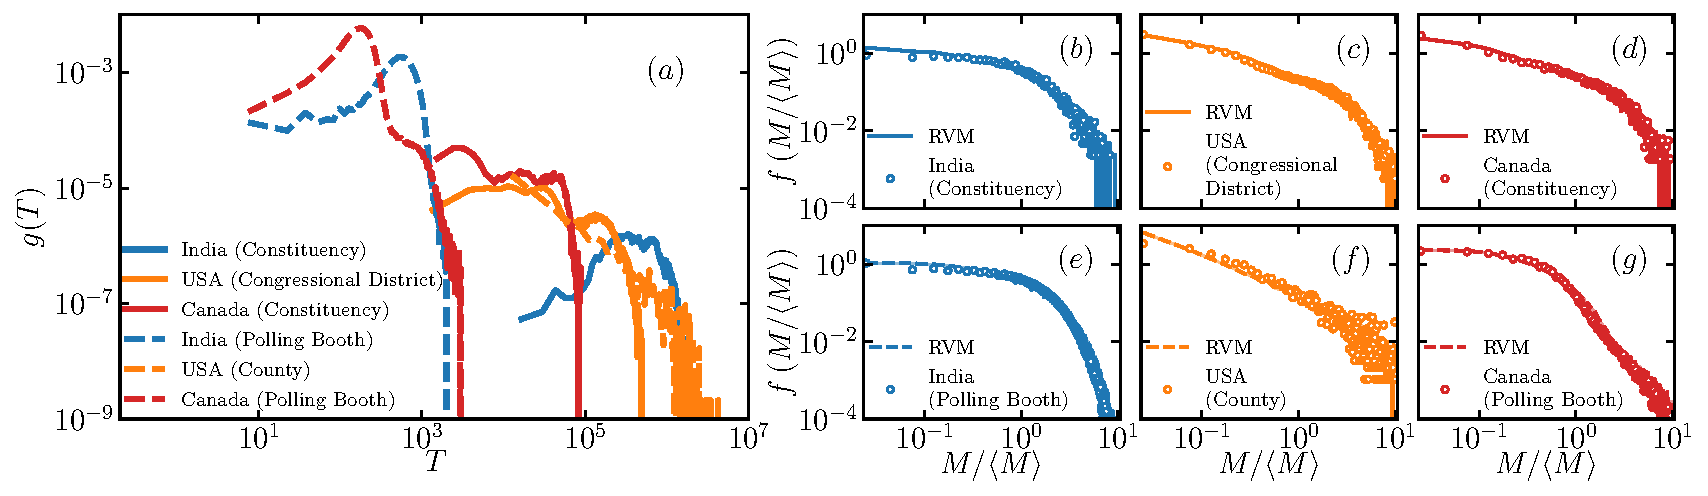
\includegraphics[width=\textwidth]{chapters/chapter4/fig_2.pdf}
    \caption{The turnout distribution $g(T)$ and scaled margin distribution $f(M/\langle M \rangle)$ for India (blue), the USA (orange), and Canada (red), at two widely different scales, {\it i.e.}, size of electoral units. (a) $g(T)$ at two different scales for each country. The dashed line is for smaller scales (polling booth for India and Canada, County for the USA), while the solid line represents a larger scale (constituency for India and Canada, congressional district for the USA). (b-g) $f(M/\langle M \rangle)$ from election data (open circles). Despite the differences in scale and shape of $g(T)$, the empirical $f(M/\langle M \rangle)$ shows certain consistent patterns, though scale effects are still evident.}
    \label{fig:scale_independence}
\end{figure}

The corresponding scaled margin distributions $f(M/\langle M \rangle)$ are shown in Figure \ref{fig:scale_independence}(b-g). Figure \ref{fig:scale_independence}$(b, c, d)$ shows the empirical distribution of scaled margins (in national elections) at the constituency-level scale, and Figure \ref{fig:scale_independence}$(e, f, g)$ shows the same at the scale of polling booths (county for USA). For each country, the distributions at different scales show certain similarities but also notable differences. For instance, in the USA, the county-level distribution (Figure \ref{fig:scale_independence}(f)) displays a heavier tail compared to the congressional district level (Figure \ref{fig:scale_independence}(c)), reflecting the influence of the underlying turnout distribution. Similar scale-dependent effects are visible in the data from India and Canada.

This is particularly evident for the USA, where the county-level turnout distribution shows a heavy-tailed decay, which is reflected in the corresponding scaled margin distribution (Fig.~\ref{fig:scale_independence}(f)). The faster decay at congressional district level distribution (Fig.~\ref{fig:scale_independence}(c)) is also observed. For Canada too, the empirical scaled margin distributions are noticeably different at two different scales. 

These observations suggest that while the scaled margin $M/\langle M \rangle$ brings us closer to universality than raw margins, it still carries the imprint of the underlying turnout distribution and is affected by the scale of electoral units. This motivates us to seek a more fundamental measure that might transcend these differences.

\section{The "Aha!" Moment: The Scaled Margin-to-Turnout Ratio}

Given the observed dependencies between margins and turnouts, and the constraint that $M \leq T$, we consider a new measure: the specific margin $\mu = M/T$. This ratio represents the margin normalized by the turnout at each electoral unit, producing a dimensionless measure of electoral competitiveness that is independent of the size of the electorate. This is a turnout-independent measure of electoral competitiveness and does not depend on the size of the electorate.

The specific margin $\mu$ ranges from 0 to 1, where values close to 0 indicate extremely competitive elections (nearly tied results), and values approaching 1 represent complete consensus (where nearly all voters chose the same candidate). By normalizing the margin by the local turnout, we effectively remove the scale dependency that affected our earlier analysis.

\subsection{Universal Distribution of Scaled Specific Margin}

The true breakthrough comes when we examine the scaled specific margin $x = \mu/\langle\mu\rangle$, where $\langle\mu\rangle$ is the average specific margin for each country. Figure \ref{fig:universality}(b) shows the distribution $F(x)$ of this scaled specific margin computed from electoral data across 32 countries.

\begin{figure}[H]
    \centering
    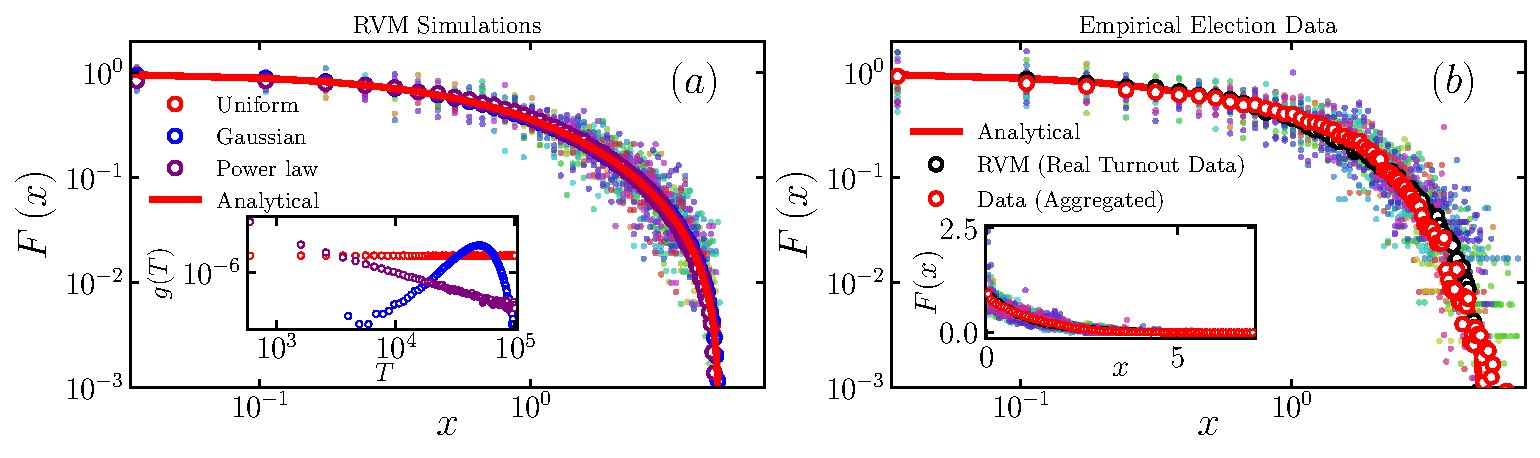
\includegraphics[width=\textwidth]{chapters/chapter4/fig_3.pdf}
    \caption{(a) Distributions of scaled specific margin $x=\mu/\langle\mu\rangle$ for different initial distributions (inset). Despite different initial distributions, a common pattern emerges. (b) The empirical distribution of $x=\mu/\langle \mu \rangle$ from election data of 32 countries (excluding Ethiopia and Belarus). Each color indicates a specific country for which the empirical election data is consolidated over several elections. The average of these empirical distributions (red open circles) reveals a striking universality. The inset depicts the distributions on a linear scale.}
    \label{fig:universality}
\end{figure}

Remarkably, Figure \ref{fig:universality}(b) reveals that the distribution $F(x)$ collapses onto a single universal curve across all 32 countries, despite vast differences in their electoral systems, cultural contexts, and historical backgrounds. Each colored point in the figure represents a specific country's data, and while there are small fluctuations around the universal curve (attributable to finite-size effects), the overall pattern is strikingly consistent. The average of all these empirical distributions, shown as red open circles, follows a smooth curve that appears to be independent of country-specific details.

The empirical distribution for each of the $32$ countries (denoted by the solid-colored circles) closely follows the trend of $F(x)$, albeit with some fluctuations induced by the finite size of data. Empirical distributions shown in the inset of Fig.~\ref{fig:universality}(b) demonstrate that at large $x$, the absolute fluctuations decrease. 

This represents a profound discovery: despite the immense complexity and diversity of electoral systems worldwide, the scaled specific margin follows a universal distribution. This suggests that the fundamental process of electoral competition—when appropriately normalized—follows the same statistical pattern regardless of where or how the election takes place.

\section{The Challenge: Can We Explain This Universality?}

While the empirical universality we've discovered is compelling, it raises a fundamental question: Why does this universal pattern emerge across such diverse electoral systems? What underlying mechanism could generate such consistent statistical behavior despite the vast differences in political contexts, voter behaviors, and electoral rules?

To obtain analytical insight, we can consider elections with three candidates in the limit of large turnout ($T \gg 1$). The votes received by $j$-th candidate can be approximated as $v_j \approx p_jT$, and the margin as $M \approx \left(p_{(3)} - p_{(2)}\right) T$, where $p_{(k)}$ denotes $k$-th order statistics of the probabilities assigned to the candidates. Evidently, in this limit, $\mu \approx p_{(3)} - p_{(2)}$ and its distribution has no explicit dependence on $T$. With this insight, the distribution of specific margins can be expressed as:

\begin{equation}
    P(\mu) = \frac{(1 - \mu)(5 + 7\mu)}{(1 + \mu)^2(1 + 2\mu)^2}
\end{equation}

Thus, the distribution $F(x)$ of the scaled specific margin $x = \mu/\langle\mu\rangle$ is:

\begin{equation}
    F(x) = \langle\mu\rangle P(x\langle\mu\rangle)
\end{equation}

with $\langle\mu\rangle = \frac{1}{2} + \ln\left(\frac{9\sqrt[4]{3}}{16}\right)$.

Remarkably, this distribution is independent of the details of the turnout distribution $g(T)$. This explains why the empirical data from vastly different countries collapses onto a single curve—the underlying statistical pattern transcends the specifics of any particular electoral system or turnout pattern.

The universality in Fig.~\ref{fig:universality} suggests that irrespective of the finer details of election processes, the mechanism underlying the core component of any competitive election -- choosing one candidate from many contenders -- leads to a universal distribution for the scaled specific margin $x=\mu/\langle \mu \rangle$.

\subsection{A Glimpse of the Mechanism: Setting Up the Random Voting Model}

The consistency of the pattern suggests that there might be a simple but powerful statistical principle at work—something fundamental to the process of competitive selection itself, rather than specific to electoral politics. The universality we've discovered hints that once turnout is "normalized out" through the specific margin, what remains is a fundamental statistical process common to all competitive elections. 

This suggests that a minimal model focused on the core statistical features of electoral competition might be sufficient to explain the observed universality. Such a model would need to capture the essential statistical features of electoral competition without relying on detailed assumptions about voter psychology, campaign dynamics, or specific electoral rules. Instead, it would focus on the basic structure of competitive selection processes, where multiple candidates compete for a finite number of votes.

In the next chapter, we will introduce precisely such a model—the Random Voting Model (RVM)—which explains this universality from first principles and makes additional predictions about electoral statistics across different scales and contexts. This parameter-free model demonstrates how the distribution of margins is fundamentally driven by the turnout distribution, yet the scaled specific margin follows a universal pattern independent of turnout.

\section{Conclusion: Universality as a Signature of Democratic Competition}

In this chapter, using extensive election data from 34 countries spanning multiple decades and electorate scales, we have demonstrated universality through analysis of the margin of victory and turnout data in democratic elections. We have shown that while raw turnout distributions vary dramatically across countries and scales, and scaled margin distributions retain country-specific features, the scaled specific margin follows a universal distribution across 32 diverse democracies.

This universality transcends the particularities of individual countries, electoral systems, and scales, revealing a fundamental statistical signature that appears to be intrinsic to competitive democratic processes. Like other universalities discovered in complex systems, this pattern emerges not despite but because of the underlying complexity, as the central limit theorem emerges from the aggregation of many random variables.

Competitiveness in any election is encoded in the victory margins and turnouts. The latter also expresses people's interest in the participatory democratic process. The scaled distribution of margin-to-turnout ratio $\mu$ has a universal form for all elections independent of country, regions, turnouts and the scale of elections. This result can be regarded as a stylized fact of elections. 

The universal distribution we've identified should be considered a stylized fact of democratic elections—an empirical regularity that any successful election model must reproduce. In the next chapter, we will develop precisely such a model, demonstrating how a simple yet powerful framework can explain this universality and make additional predictions about electoral statistics across different scales and contexts.

\newpage
\thispagestyle{empty}
\mbox{}

\chapter{The Random Voting Model: When Chance Explains Choice}
\label{chap5}

In the previous chapter, we uncovered a remarkable universal pattern in electoral statistics: the scaled distribution of the specific margin (margin-to-turnout ratio) follows a consistent curve across diverse democracies, electoral systems, and scales. This universality emerged despite the vast differences in raw turnout and margin distributions across countries. We introduced the Random Voting Model (RVM) as a simple stochastic framework that remarkably captures this universal pattern with surprising accuracy.

Building on this discovery, this chapter provides a comprehensive analysis of the RVM from first principles. We will delve into its mathematical foundations, derive key analytical results, and demonstrate how this elegantly simple stochastic model can explain multiple empirical findings from electoral data. Through both analytical derivations and simulation results, we'll show that the RVM not only predicts the universal specific margin distribution but also connects turnout distributions to margin distributions across different electoral contexts.

\section{Introducing the Random Voting Model (RVM): Simplicity by Design}
\label{sec:RVM_intro}
The Random Voting Model is based on the premise that electoral outcomes can be understood through a minimal statistical framework that captures the essence of competition without modeling voter psychology or strategic behavior. The model is parameter-free beyond the turnout distribution and number of candidates, relying only on simple probabilistic principles.

In this Random Voting Model, $c_i$ number of candidates contest at $i$-th electoral unit with $n_i$ electors (voters) and each elector from the $i$-th electoral unit casts their vote for $j$-th candidate with a probability $p_{ij}$. These probabilities are assigned as follows: for each candidate, a number between $0$ and $1$ is drawn uniformly at random, which is assigned as an unnormalized probability weight $w_{ij}$ to that candidate. The weights are subsequently normalized to get the probability $p_{ij}, j = 1, 2 \dots c_i$ of receiving the vote of an elector. This can be mathematically stated as
\begin{equation}
    w_{ij} \sim \mathcal{U}(0, 1) \quad \text{and} \quad p_{ij} = \frac{w_{ij}}{\sum_k w_{ik}}, \text{ with } j = 1, 2 \dots c_i,
    \label{eq:RVM_prob}
\end{equation}
where $\mathcal{U}(0, 1)$ denotes a uniformly distributed random variable in $(0,1)$.

After each of the $n_i$ electors (voters) in $i$-th electoral unit casts their vote for some candidate $j$ independently with probability $p_{ij}$, the candidate receiving the most votes $V_{i, w}$ is declared the winner, and the candidate securing the next largest number of votes $V_{i, r}$ is the runner-up. The \emph{margin of victory} $M_i$ is then defined to be the vote difference between the winner and the runner-up: \emph{i.e.} $M_i = V_{i, w} - V_{i, r}$. The empirical election data we employ shows that the top three candidates, on average, account for nearly 87\% of all votes polled in an election.
Hence, as part of the model specification, we fix the number of candidates in each electoral unit to be three, i.e., $c_i = 3$ for all $i$.

The only input to this model is the raw turnout data, i.e., the number of voters (who actually voted) in each constituency. For the model simulation, we use the turnout data of real elections as the total number of voters in different constituencies. To understand how simulations are performed, consider this notional example: if a country has $N=100$ constituencies and data for five such elections is available. Then, the model is simulated on $500$ electoral units. The number of electors in each electoral unit is taken from the consolidated turnouts. Such a simulation of election is performed multiple times to get the average distributions.
\section{The RVM's First Symphony: Obtaining the Universal $Q_{\widetilde{\mu}}\left(\widetilde{\mu}\right)$}
\label{sec:RVM_first_symphony}
We now demonstrate how the RVM explains the universal distribution of scaled specific margin $Q_{\widetilde{\mu}}\left(\widetilde{\mu}\right)$ observed in the previous chapter. As mentioned in the previous section (\ref{sec:RVM_intro}), we consider the case where $3$ candidates are contesting in an election. The weight assigned for the $j$-th candidate of the $i$-th electoral unit is $w_{ij}$. These weights are drawn independently at random from a uniform distribution between $0$ and $1$.  The corresponding probability $p_{ij}$ of receiving votes is calculated by normalizing these weights. Hence, we have the following,
\begin{equation}
    w_{ij} \sim \mathcal{U}(0, 1) \text{ and } p_{ij} = \frac{w_{ij}}{\sum_{k=1}^3 w_{ik}}; \text{ with } j = 1, 2, 3.
\end{equation}
For the rest of the analysis in this chapter, we focus on a single ($i$-th) electoral unit with voter turnout $T$ and drop the corresponding index $i$ for brevity. Hence,
\mathtoolsset{centercolon}
\begin{equation}
    w_{ij} := w_j \text{ and } p_{ij} := p_j.
\end{equation}
\subsection{The Set-up: Large Turnout Limit}
For large turnout $(T \gg 1)$, it is reasonable to assume the number of votes received by $j$-th candidate is proportional to their probability $p_j$, in particular, $v_j \approx p_j T$. Hence, for $T \gg 1$, the \emph{margin} can be approximated as 
\begin{equation}
M \approx (p_{max} - p_{2nd \: max})T,
\end{equation}
where $p_{max}$ and $p_{2nd \:max}$ correspond to the largest and the second largest probabilities assigned to the candidates. For example, if the probabilities $p_1, p_2,$ and $p_3$ assigned to the 3 candidates are $0.1, 0.6,$ and $0.3$, then $p_{max} = p_2 = 0.6$ and $p_{2nd \:max} = p_3 = 0.3$. The margin $M$ can also be written in terms of $w_j$ as the following:
\begin{center}
\begin{align}
    \nonumber M &\approx \left(\frac{w_{max}}{w_1 + w_2 + w_3} - \frac{w_{2nd\:max}}{w_1 + w_2 + w_3}\right)T,\\
    \nonumber & = \left(\frac{w_{(3)}}{w_{(1)} + w_{(2)} + w_{(3)}} - \frac{w_{(2)}}{w_{(1)} + w_{(2)} + w_{(3)}}\right)T,\\
    & = \left(\frac{w_{(3)} - w_{(2)}}{w_{(1)} + w_{(2)} + w_{(3)}}\right)T,
\end{align}

\end{center}
where $w_{(k)}$ is the $k$-th order statistics \cite{BarBalNag2008}. Hence, 
\begin{center}
\begin{align}
    \frac{M}{T} \approx \frac{w_{(3)} - w_{(2)}}{w_{(1)} + w_{(2)} + w_{(3)}}.
    \label{eq:S6}
\end{align}
\end{center}
\subsection{Order Statistics: The Key to Understand Ranking}
Consider $n$ \emph{iid} random variables $\{X_1, X_2 \dots X_n\}$ drawn from a distribution $\rho(x)$. When arranged in ascending order, the random variable at the $k$-th spot is defined as the $k$-th order statistics. In particular, $n$-th and $1$-st order statistics correspond to the maximum and minimum of those $n$ random variables, respectively. The $k$-th order statistics of the random variable $X$ is denoted by $X_{(k)}$.

The joint probability density of all the order statistics of the above-mentioned $n$ random variables, $\mathbbm{P}\left(x_{(1)}, x_{(2)}, ... x_{(n)}\right)$, defined as the probability density that the random variable $X_{(k)}$ takes the value $x_{(k)}$ for $k \in \{ 1, 2, \dots, n\}$, is
\begin{equation}
    \mathbbm{P}\left(x_{(1)}, x_{(2)}, ... x_{(n)}\right) = n!\prod_{k=1}^{n}\rho\left(x_{(n)}\right).
\end{equation}
\subsection{Back to Reality: RVM's First Symphony}
Now that we understand the joint probability density of the order statistics, for RVM, we have $n = 3$ and $\rho(x) = \mathcal{U}(0, 1)$. Hence we have,    
\begin{center}
    \begin{align}
        \mathbbm{P}\left(w_{(1)}, w_{(2)}, w_{(3)}\right) = 3! = 6; \text{ with } 0<w_{(1)}<w_{(2)}<w_{(3)}<1,
    \end{align}
\end{center}
and $\mathbbm{P}\left(w_{(1)}, w_{(2)}, w_{(3)}\right) = 0$ otherwise, with the following normalization:
\begin{equation}
    \int_{0}^{1}dw_{(3)}\int_{0}^{w_{(3)}}dw_{(2)}\int_{0}^{w_{(2)}} 6 dw_{(1)} = 1.
\end{equation}
From the joint probability distribution of all the order statistics, we calculate the approximate probability density function of specific margin $ M / T = \mu$ from Eq.~\eqref{eq:S6} as follows, 
\begin{center}
    \begin{align}
        \nonumber Q_{\mu}\left(\mu\right) & = 6 \nonumber \int_{0}^{1}dw_{(3)}\int_{0}^{w_{(3)}}dw_{(2)}\int_{0}^{w_{(2)}} \delta\left(\mu - \frac{w_{(3)}- w_{(2)}}{w_{(1)} + w_{(2)} + w_{(3)}}\right)dw_{(1)},\\
        & = 6 \int_{0}^{1}dw_{(3)}\int_{0}^{w_{(3)}} \frac{w_{(3)} - w_{(2)}}{\mu^2} \nonumber \mathbbm{1}_{0<\frac{w_{(3)} - \mu w_{(3)} - (1 + \mu)w_{(2)}}{\mu}<w_{(2)}} dw_{(2)},\\
        & = 6 \int_{0}^{1}dw_{(3)} \frac{(1 - \mu)(5 + 7\mu)w_{(3)}^2}{2(1 + \mu)^2(1 + 2\mu)^2}.\\
    \end{align}
\end{center}
Finally, after performing this integral, we get 
\begin{equation}
    Q_{\mu}\left(\mu\right) = \frac{(1 - \mu)(5 + 7\mu)}{(1 + \mu)^2(1 + 2\mu)^2}.
\end{equation}
The distribution $Q_{\mu}\left(\mu\right)$ does not depend on the turnout and is universal. Now, by a change of variable to scaled specific margin defined as $\widetilde{\mu} = \mu / \langle \mu \rangle$, we obtain its distribution $Q_{\widetilde{\mu}}\left(\widetilde{\mu}\right)$ to be
\begin{equation}
    Q_{\widetilde{\mu}}\left(\widetilde{\mu}\right) = \langle \mu \rangle ~ Q_{\mu}\left( \widetilde{\mu} \langle \mu \rangle \right) =  \frac{\langle \mu \rangle(1 - \widetilde{\mu} \langle \mu \rangle)(5 + 7\widetilde{\mu} \langle \mu \rangle)}{(1 + \widetilde{\mu} \langle \mu \rangle)^2(1 + 2\widetilde{\mu} \langle \mu \rangle)^2}, 
\end{equation}
where $\langle \mu\rangle = \frac{1}{2}+\ln \left(\frac{9 \sqrt[4]{3}}{16}\right)$.
This derived distribution $Q_{\widetilde{\mu}}\left(\widetilde{\mu}\right)$ is precisely the universal curve observed in the empirical data across 32 countries in the previous chapter. The remarkable agreement between theory and data as shown in Fig.~\ref{fig:RVM_mu} confirms that the RVM captures the essential statistical features underlying electoral competition.

\begin{figure}[H]
    \centering
    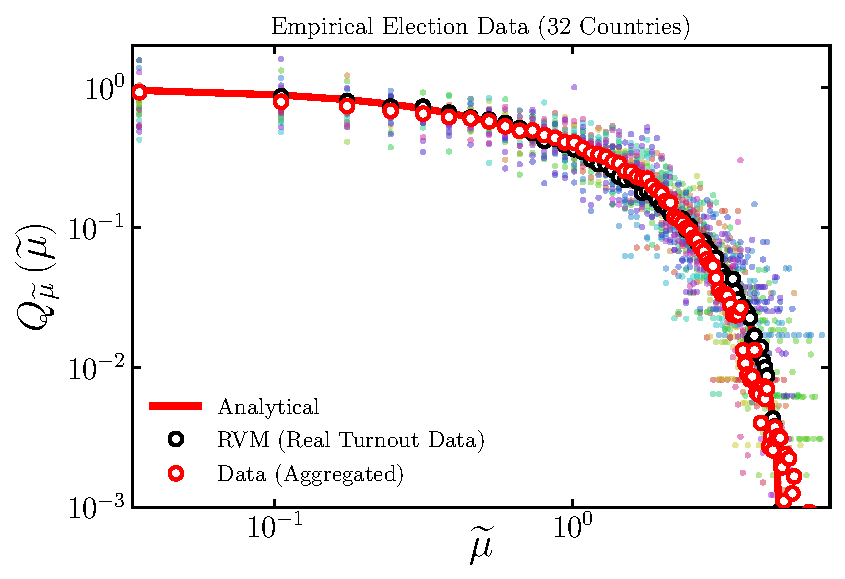
\includegraphics[width=0.95\textwidth]{chapters/chapter5/universality_empirical_analytical.pdf}
    \caption{$Q_{\widetilde{\mu}}\left(\widetilde{\mu}\right)$: The distribution is universal and does not depend on the turnout distribution. Each color indicates empirical $Q_{\widetilde{\mu}}\left(\widetilde{\mu}\right)$ for a specific country for which the election data is consolidated over several elections. The average of these empirical distributions (red open circles) closely follows the analytical curve (red line) and the averaged RVM predictions for each country (black open circles).}
    \label{fig:RVM_mu}
\end{figure}

\section{Expanding the Repertoire: Predicting Margins from Turnouts}
Having established that the RVM predicts the universal specific margin distribution, we now explore how the model can predict the margin distribution $Q_M(M)$ from an arbitrary turnout distribution $g(T)$. From the previous section, we have the distribution of the specific margin $\mu = M / T$ to be
\begin{equation}
    Q_{\mu}\left(\mu\right) = \frac{(1 - \mu)(5 + 7\mu)}{(1 + \mu)^2(1 + 2\mu)^2}.
\end{equation}
Through a simple change of variable $(M = \mu T)$ we get,
\begin{equation}
    \mathcal{P}(M|T) = \frac{(1 - M / T)(5 + 7M /T)}{T(1 + M / T)^2(1 + 2M / T)^2}.
\end{equation}
For an arbitrary turnout distribution $g(T)$, we obtain the distribution of $M$ to be,
\begin{equation}
    Q_M(M) = \int_{M}^{\infty}g(T)\mathcal{P}(M |T) dT = \int_{M}^{\infty}g(T)\frac{(1 - M / T)(5 + 7M /T)}{T(1 + M / T)^2(1 + 2M / T)^2} dT.
\end{equation}
Again with $u = T / M$, the above integral transforms to,
\begin{equation}
    Q_M(M) = \int_{1}^{\infty}g(Mu)\frac{u(u - 1)(5u + 7)}{(1 + u)^2 (2 + u)^2}du.
    \label{eq:pm}
\end{equation}
\subsection{Turnout Distribution Effects on Margin Distribution}
We compute $Q_M(M)$ for different turnout distributions $g(T)$. In particular, we take $g(T)$ to be (A) exponential, (B) power law, and (C) Gaussian distributions as they have vastly different tail behaviors. Finally we also consider a uniform turnout distribution with finite support.
\subsubsection{Exponential Turnout Distribution}
In this case $g(T) = \frac{1}{\tau}e^{-T / \tau}$, with $ \tau> 0$. Hence,
\begin{equation}
    Q_M(M) = \int_{1}^{\infty}\frac{1}{\tau}e^{-Mu / \tau} \frac{u(u - 1)(5u + 7)}{(1 + u)^2 (2 + u)^2}du,
\end{equation}
or,
\begin{equation}
    Q_M(M) = \frac{e^{-\frac{M}{\tau}}}{\tau^2} \left(4 e^{\frac{2 M}{\tau}} (\tau+M) \text{Ei}\left(-\frac{2 M}{\tau}\right)-9 e^{\frac{3 M}{\tau}} (\tau+2 M) \text{Ei}\left(-\frac{3 M}{\tau}\right)-4 \tau\right), 
\end{equation}
where $\text{Ei}(x) = \int_{-\infty}^{x}\frac{e^t}{t}dt$. At large margin limit $(M \rightarrow \infty)$, the asymptotic behavior of the distribution is the following (up to the leading order of $M$):
\begin{equation}
    Q_M(M)= \frac{\tau}{3M^2}e^{-M/\tau}.
\end{equation}
This suggests that in the large margin limit, both the margin and its corresponding turnout distribution have an exponential decay with the same rate.
\subsubsection{Power law Turnout Distribution}
In this case $g(T) = \frac{\alpha - 1}{T_{min} ^{1 -\alpha}} T ^ {-\alpha}$, with $\alpha > 1$ and $T>T_{min}$. Hence we have,
\begin{equation}
    Q_M(M) = \int_{1}^{\infty}\frac{\alpha - 1}{T_{min} ^{1 -\alpha}} (Mu) ^ {-\alpha} \frac{u(u - 1)(5u + 7)}{(1 + u)^2 (2 + u)^2}du,
\end{equation}
or,
\begin{equation}
    Q_M(M) = C(M)\frac{\alpha - 1}{T_{min} ^{1 -\alpha}} (M) ^ {-\alpha}, 
    \label{eq:powerlaw}
\end{equation}
where,
\begin{numcases}{C(M) = }
    I_1(\infty) - I_1(T_{min} / M) , \text{if } M\leq T_{min}\\
    I_1(\infty) - I_1(1), \text{otherwise,}
\end{numcases}
with,
\begin{equation}
    I_1(y) = \int \frac{y^{1 - \alpha}(y - 1)(5y + 7)}{(1 + y)^2 (2 + y)^2}dy,
\end{equation}
and,
\begin{numcases}{I_1(y)=}
     -\frac{4}{y+1}+\frac{9}{2 (y+2)}-\frac{1}{4} 7 \ln (y)+4 \ln (y+1)-\frac{9}{4} \ln (y+2), \text{if } \alpha = 2 \\
     \frac{y^{2-\alpha } \left(16 \, _2F_1(2,2-\alpha ;3-\alpha ;-y)-9 \, _2F_1\left(2,2-\alpha ;3-\alpha ;-\frac{y}{2}\right)\right)}{4 (\alpha -2)}, \text{otherwise,} \\
\end{numcases}
where ${}_{2}F_{1}(a,b;c;z)$ is a hypergeometric function \cite{abramowitz_stegun}, defined as,
\begin{align*}
    {\displaystyle {}_{2}F_{1}(a,b;c;z)  =\sum _{n=0}^{\infty }{\frac {(a)_{n}(b)_{n}}{(c)_{n}}}{\frac {z^{n}}{n!}}=1+{\frac {ab}{c}}{\frac {z}{1!}}+{\frac {a(a+1)b(b+1)}{c(c+1)}}{\frac {z^{2}}{2!}}+\cdots .}\\
\end{align*}

It is evident from Eq.~\eqref{eq:powerlaw} that for $M > T_{min}$, the margin distribution decays with a power law exponent $\alpha$, exactly the same as the turnout distribution.
\subsubsection{Gaussian Turnout Distribution}
In this case $g(T) = C_0 e^{-(T/T_0)^2}$, with $T>0$. Hence,
\begin{equation}
     Q_M(M) = \int_{1}^{\infty} C_0 e^{-(Mu/T_0)^2}\frac{u(u - 1)(5u + 7)}{(1 + u)^2 (2 + u)^2}du.
\end{equation}
At large margin limit $(M \rightarrow \infty)$, the asymptotic behavior of the distribution is the following (up to the leading order of $M$):
\begin{equation}
    Q_M(M) = \frac{C_0}{12}\left(\frac{T_0}{M}\right)^4 e^{-\left(M/ T_0\right)^2}, 
\end{equation}
and it has a Gaussian decay similar to the corresponding turnout distribution.\\

From the asymptotic analysis of the margin distributions for the three above-mentioned turnout distributions, we provide strong evidence that the tails of the margin distributions mimic that of the corresponding turnout distribution. For completeness, we also compute the margin distribution corresponding to a uniform turnout distribution which has a finite support (no tail behavior).
\subsubsection{Uniform Turnout Distribution}
In this case $g(T) = \frac{1}{b - a}$, when $T \in [a, b]$, otherwise  $g(T) = 0$. Hence,
\begin{numcases}{Q_M(M)= }
    \frac{1}{b - a}\int_{a/M}^{b/M}\frac{u(u - 1)(5u + 7)}{(1 + u)^2 (2 + u)^2}du , \text{if } M\leq a\\
    \frac{1}{b - a}\int_{1}^{b/M}\frac{u(u - 1)(5u + 7)}{(1 + u)^2 (2 + u)^2}du, \text{otherwise,}
\end{numcases}
or, 
\begin{numcases}{Q_M(M)= }
    \frac{1}{b - a} \left(I_2(b / M) - I_2(a / M)\right), \text{if } M\leq a\\
    \frac{1}{b - a}\left(I_2(b / M) - I_2(1)\right),  \text{if } a > M \geq b\\
    0,  \text{ otherwise,}
\end{numcases}
where, 
\begin{equation}
    I_2(y) = \int \frac{y(y - 1)(5y + 7)}{(1 + y)^2 (2 + y)^2}dy = -\frac{4}{y+1}+\frac{18}{y+2}-4 \ln (y+1)+9 \ln (y+2).
\end{equation}
\subsection{RVM Simulations with Synthetic Turnout Distributions}
The RVM enables us to estimate the scaled margin distribution $f(M / \langle M \rangle)$ using only the raw turnout data, indicating that $f(M / \langle M \rangle)$ is driven by the details of the turnout distribution $g(T)$. To further quantify the effect of $g(T)$ on the scaled margin distribution $f(M / \langle M \rangle)$, we simulate elections using RVM, with turnouts drawn from vastly different synthetically generated distributions. In particular, to study the tail behaviors, we use the following four different turnout distributions:
\begin{enumerate}
    \item \textbf{Gaussian Turnout Distribution:} $g(T) = \frac{1}{\sigma\sqrt{2\pi}}\exp\left(-\frac{(T - \mu)^2}{2\sigma^2}\right), \text{ with } \mu = 50000$, $\sigma = 10000$ and $T > 0$.
    \item \textbf{Exponential Turnout Distribution:} $g(T) = \frac{1}{\tau} \exp{\left(-\frac{T}{\tau}\right)}, \text{ with } \tau = 50000$.
    \item \textbf{Power law Turnout Distribution:} $g(T) = \frac{\alpha - 1}{T_{min} ^{1 -\alpha}} T ^ {-\alpha}$, with $\alpha = 2$ and $T_{min} = 100$ (minimum possible turnout).
    \item \textbf{Uniform Turnout Distribution:} $T \sim \mathcal{U} (a, b)$, with $a = 100$ and $b = 100000$. $\mathcal{U}(a, b)$ denotes uniform distribution between the range $a$ and $b$.
\end{enumerate}

Each of the RVM simulations was performed on $10^6$ electoral units, with turnouts (rounded down to the nearest integer) drawn from one of these three distributions. The simulation demonstrates that the tail of the margin distribution mimics the turnout distribution's tail.  This is evident in Fig.~\ref{fig_sup_1}(a), (b), and (c). The tail of the margin distribution (Fig.~\ref{fig_sup_1} (c)) corresponding to power law turnouts decays with the same power law exponent.  In the simulation with Gaussian turnout distribution, we find the tail of the margin distribution also has a Gaussian falloff (Fig.~\ref{fig_sup_1} (a)). Similarly, the margin distribution corresponding to exponential turnouts has an exponential tail (Fig.~\ref{fig_sup_1} (b)). As the probability density function of uniform turnout distribution and corresponding margin distribution have finite supports, their tails can not be properly defined. We find a sharp cutoff in the corresponding margin distribution. The analytical (semi-analytical for Gaussian turnout) predictions for the margin distributions (shown as black lines in Fig.~\ref{fig_sup_1}) corresponding to all four aforementioned turnout distributions are in excellent agreement with the RVM simulation. In empirical county-level election data of the United States, the heavy-tailed decay of the turnout distribution is reflected in the corresponding margin distribution (Fig.~\ref{fig_sup_1}(e)). In Fig.~\ref{fig_sup_1} (f), we see a similar decay trend in both margin and turnout distribution, which correspond to congressional district-level election data of the USA. We obtain the scaled margin distribution $f(M / \langle M \rangle)$ by scaling $Q(M)$ by its mean; hence, both $Q(M)$ and $f(M / \langle M \rangle)$ have similar decay and are strongly related to the corresponding turnout distribution $g(T)$.
\begin{figure}[H]
    \centering
    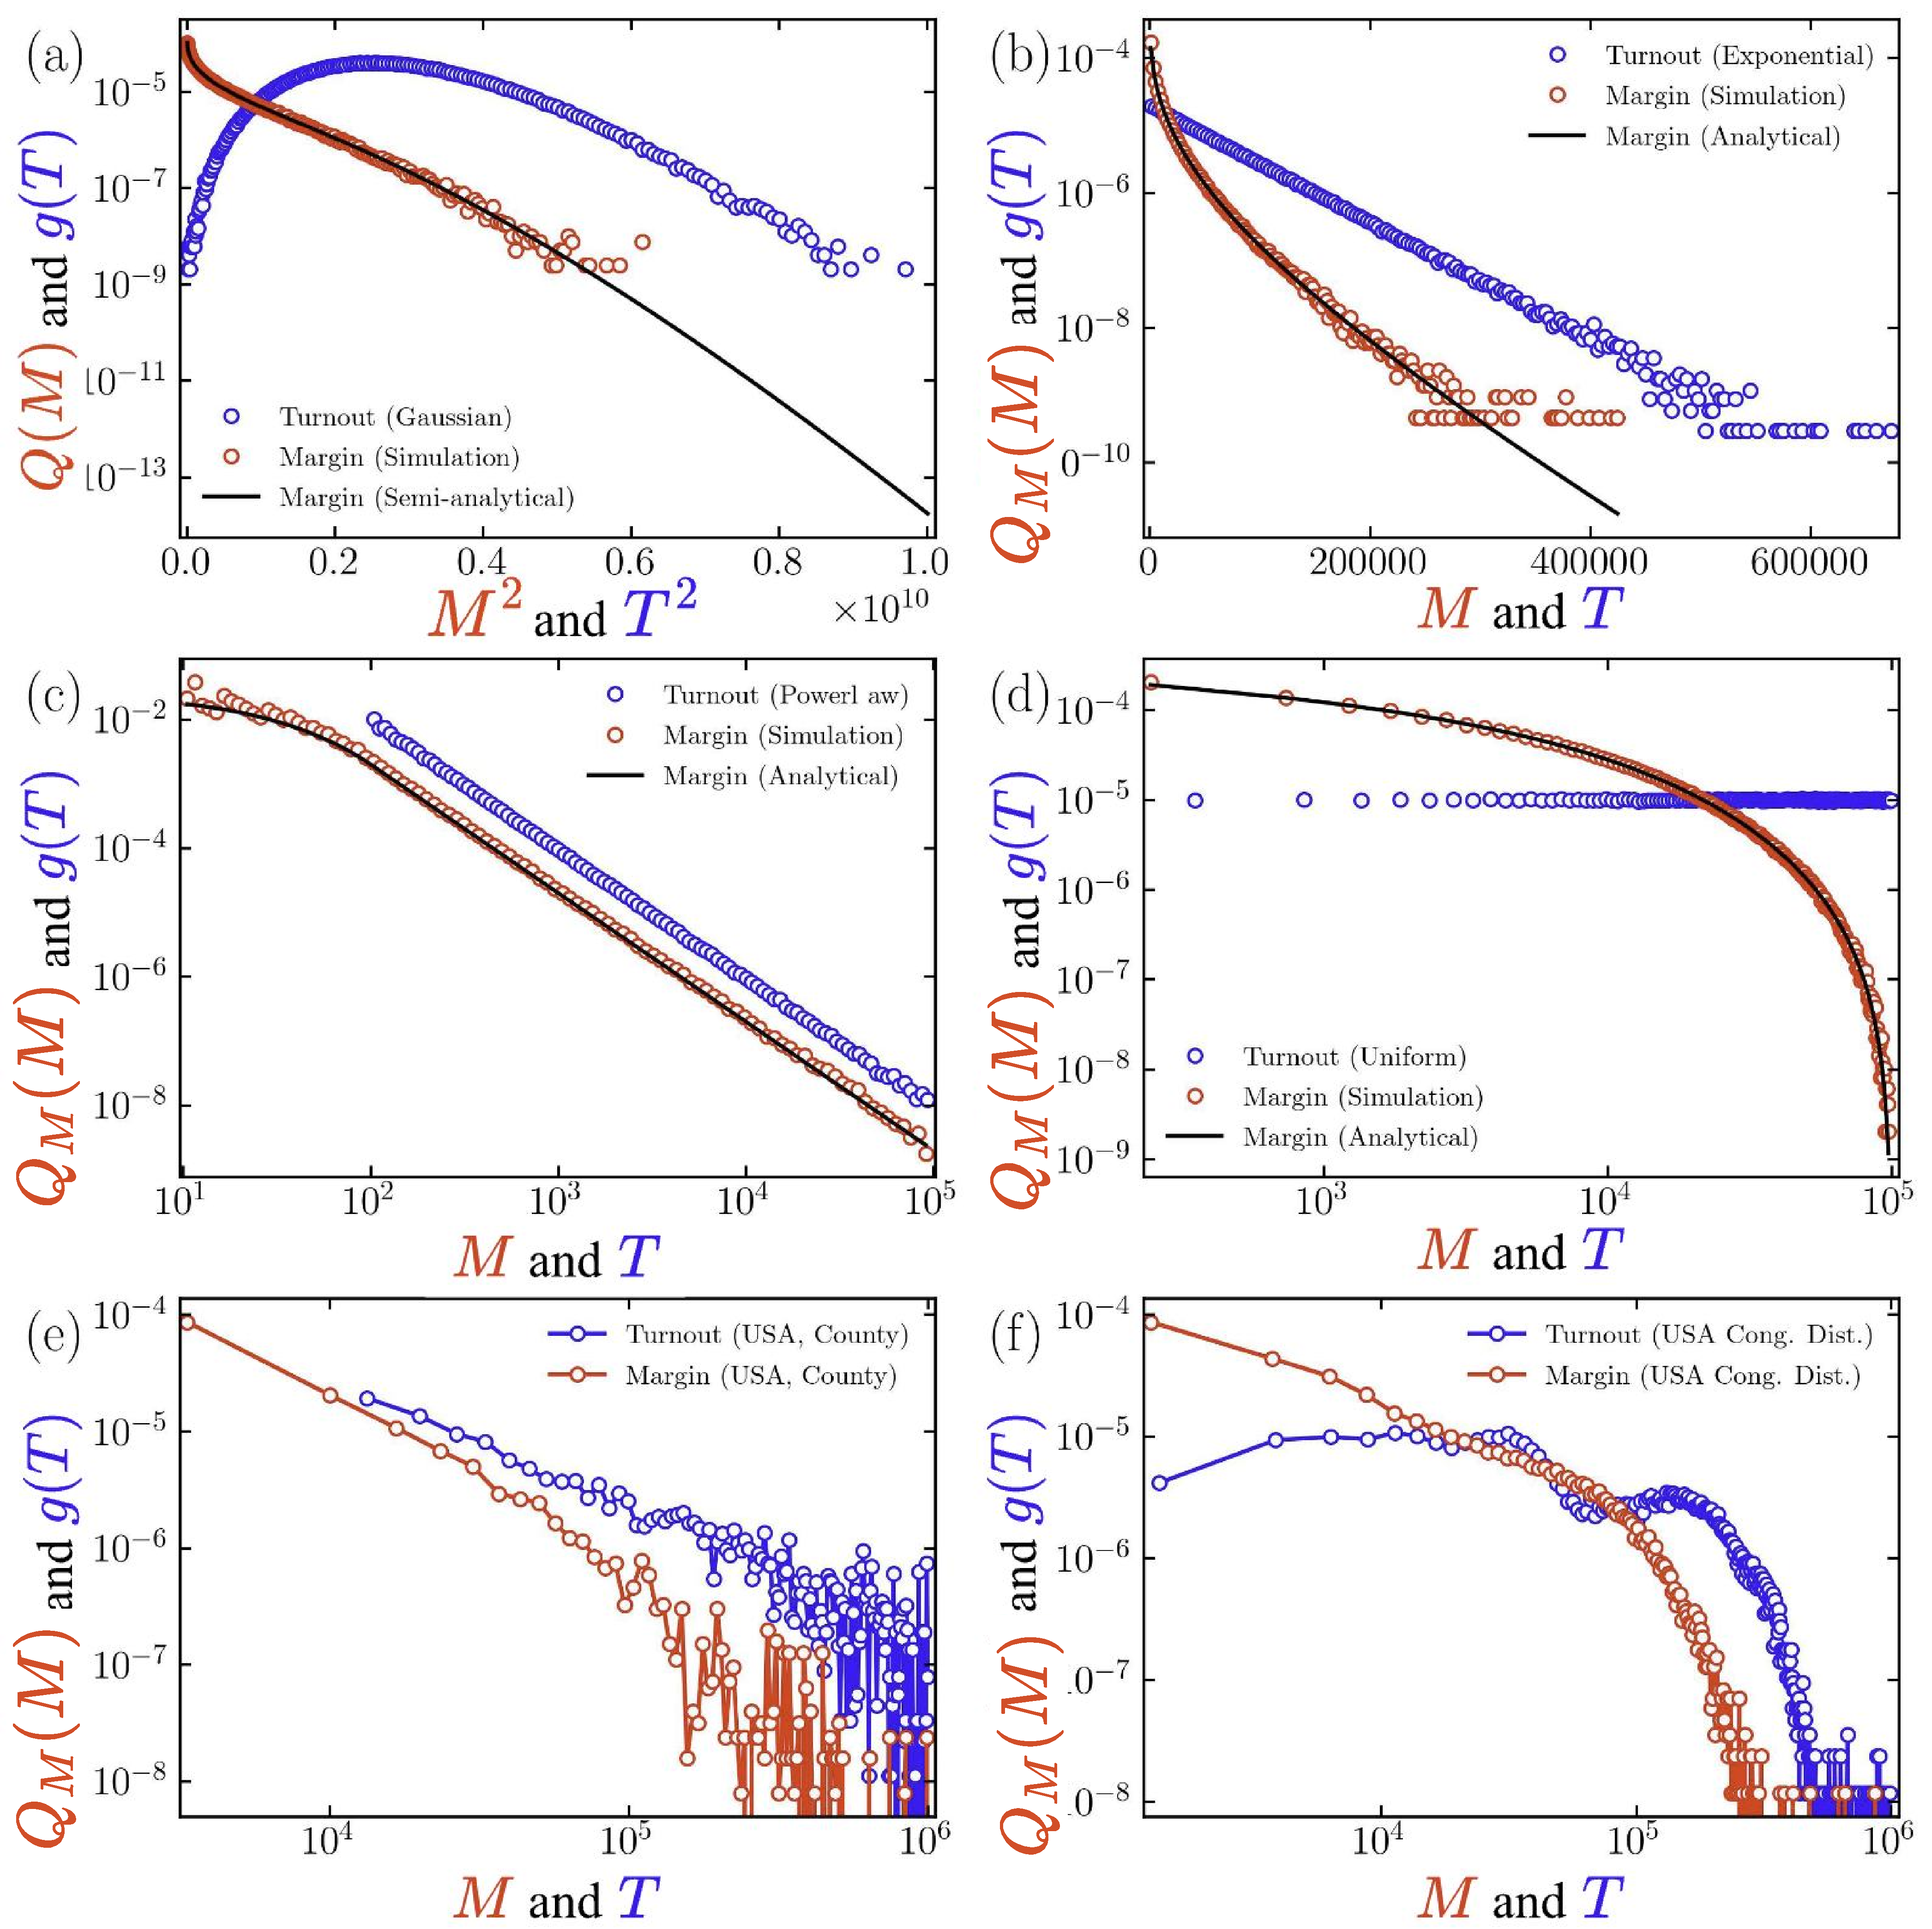
\includegraphics[width=\textwidth]{chapters/chapter5/margin_turnout_dists.pdf}
    \caption{The margin distribution $Q(M)$ is plotted with the corresponding turnout distribution $g(T)$ to demonstrate that the tails of both these distributions are correlated. Panels (a), (b), (c), and (d) correspond to Gaussian, exponential, power law, and uniform turnout distributions, respectively. Blue open circles denote the turnout distributions. Red open circles denote the margin distribution computed through RVM simulations. Black solid lines correspond to the margin distribution computed using Eq.~\ref{eq:pm}. For exponential, power law, and uniform turnout distributions, the integration was analytically calculated, and for Gaussian turnout distribution, it was evaluated numerically. Panels (e) and (f) depict the margin and turnout distribution for the county-level and congressional district-level election data of the USA, respectively.}
    \label{fig_sup_1}
\end{figure}
\subsection{Need of the Hour: Scaling by Mean}
RVM can remarkably predict the overall trend, especially the tail behaviors of the margin distributions $Q_M(M)$. However, the prediction of the whole distribution is sadly not possible, due to RVM's inability of relaiably prediting the mean margin. To surcumnavigate this limitaion, we scale the margin distributions with their sample mean, 

\subsubsection{PC}
% paraphrase
Figure \ref{fig_1}(a) displays the distribution of raw turnout $g(T)$ at the constituency level for national elections in six countries, namely, India, USA, South Korea, Canada, Japan, and Germany. Striking dissimilarities in $g(T)$ are visible in the shape and support of distribution for countries. For Germany, $g(T)$ has a unimodal character, while that for Canada and the USA display multiple peaks. The corresponding scaled margin $M/\langle M \rangle$ is displayed as distribution $f(M/\langle M \rangle)$ (computed from the consolidated margin data for each country) in Fig.~\ref{fig_1}(b-g). While they appear to be broadly similar, certain differences are clearly noticeable. In particular, $f(M/\langle M \rangle)$ for German elections in Fig.~\ref{fig_1}(g) has a sharp cutoff, but for India and Japan in Fig.~\ref{fig_1}(b, f) the distribution has a slower decay. These observations motivate the questions of whether $f(M/\langle M \rangle)$ is related to the raw turnout distribution and can be obtained from it.

To investigate this question, we propose a Random Voting Model (RVM) ${\mathcal V}(T)$ that takes raw turnouts $T=\{T_1, T_2 \dots T_N\}$ as input. This model emulates an election taking place at $N$ electoral units (say, constituencies). At $i$-th unit, each of the $T_i$ voters (raw turnout at $i$-th unit) can cast only one vote, independently and by randomly choosing one of the $c_i$ contesting candidates. The probability that candidate $j$ in $i$-th unit can attract a vote is $p_{ij}= w_{ij}/\sum_k w_{ik}$, where $w_{ij} \in [0,1]$ is a random number drawn from a uniform distribution. While this protocol provides a natural and effective choice for $p_{ij}$, the sensitivity of the RVM predictions on different protocols is discussed in Sec.~S5 of Ref. \cite{supp}. In election data that we use, averaged over all the 34 countries, the top two (three) candidates account for 79\% (87\%) of all votes polled. Hence, the model assumes three candidates at every constituency: $c_i=3$ for $i=1,2 \dots N$, and that all eligible voters cast their votes, implying $T_i = n_i$. By simulating this model, margin $M_i$ is obtained for $i$-th electoral unit and $\langle M \rangle = (1/N) \sum_{i=1}^N M_i$ is the associated sample mean. For a detailed description of the model, see Sec.~S1 of Ref. \cite{supp}. 

The model predictions depend exclusively on the actual turnout distribution, and no free parameters to be tuned. As illustrated in Fig.~\ref{fig_1}(b - g), the scaled margin distributions predicted by this model (solid lines) show a remarkable agreement with those computed from empirical margin data from real elections. Notably, RVM faithfully captures disparate decay features in  $f(M/\langle M \rangle)$ for India, USA, South Korea, Canada, Japan, and Germany (for 28 other countries, see Sec.~S7 of Ref. \cite{supp}). This suggests that the raw turnout data carries intrinsic information about the margin distribution. RVM effectively leverages this information embedded in the turnout distribution to predict the scaled margin distribution. 
\begin{figure}
    
\end{figure}
\subsubsection{Different Scale}
Next, we show that these results are independent of the number of voters or size of electoral units. In large countries, depending on the size of the electoral unit, the typical turnout can differ by several orders of magnitude. For example, in India, polling booths have a typical electoral size $\sim 10^3$, whereas, at the parliamentary constituency level, it is about $10^6$. Further, the shapes of $g(T)$ are also vastly different at different scales. Figure \ref{fig_2}$(a)$ captures the striking differences in range and shape of $g(T)$ for India, the US, and Canada at two different scales. Quite remarkably, despite these vast differences in the scale, the same RVM ${\mathcal V}(T)$, without any parameter adjustments, accurately predicts the scaled margin distribution. Figure \ref{fig_2}$(b, c, d)$ shows the empirical distribution of scaled margins (in national elections) at the constituency-level scale, and Figure \ref{fig_2}$(e, f, g)$ shows the same at the scale of polling booths (county for USA).

\begin{figure}
    
\end{figure}

\subsubsection{All 32 Countries}
Further in figure X we demonstrate the remarkable prediction scaled margin distributions by RVM.

\begin{figure}
    
\end{figure}

\section{Conclusion: The Power and Limitations of RVM}

In this chapter, we have provided a comprehensive analysis of the Random Voting Model (RVM) from its first principles. We demonstrated how this elegantly simple model generates the universal distribution of scaled specific margins observed across diverse electoral systems worldwide. Through rigorous mathematical derivations, we showed that the model successfully predicts this universality without requiring any parameters beyond the turnout distribution and number of candidates.

Furthermore, we established that the RVM provides powerful insights into how turnout distributions shape margin distributions across different electoral contexts. Through both analytical solutions and simulations with various synthetic turnout distributions (Gaussian, exponential, power law, and uniform), we demonstrated that margin distributions inherit the tail behavior of their corresponding turnout distributions. This finding explains why electoral margin distributions can vary dramatically across countries while still adhering to the universal specific margin pattern.

The model's ability to predict scaled margin distributions from raw turnout data alone—without any adjustments or free parameters—is remarkable and represents a significant advance in our understanding of electoral statistics. It suggests that beneath the apparent complexity and diversity of electoral systems worldwide lies a fundamental statistical principle that governs competitive selection processes.

However, the RVM also has limitations. While it excellently predicts the shape and tail behavior of margin distributions, it struggles to reliably predict the mean margin. This necessitates scaling by empirical means when comparing model predictions to real-world data. Additionally, the model's simplified assumption of random voting does not account for strategic voting behavior, partisan affiliations, or other psychological and sociological factors that influence real elections.

Despite these limitations, the success of this minimal statistical model in capturing key universal features of electoral competition demonstrates the power of stochastic approaches in understanding complex social phenomena. It reveals that certain macroscopic patterns in electoral systems may be governed more by basic statistical principles than by the intricacies of voter psychology or electoral rules.

In the next chapter, we will build upon this foundation to explore how deviations from the universal pattern predicted by RVM might serve as indicators of electoral anomalies or potential fraud. By establishing a statistical baseline for "typical" electoral competition, we gain a powerful tool for detecting unusual patterns that may warrant closer scrutiny. This approach may ultimately provide a data-driven, politically neutral method for monitoring electoral integrity worldwide.
\newpage
\thispagestyle{empty}
\mbox{}

\chapter{From Theory to Practice: Applications and Interventions}
\label{chap6}

Having established the theoretical foundations of the Random Voting Model and demonstrated its remarkable predictive power across diverse electoral contexts, we now turn our attention to practical applications. This chapter explores how our theoretical insights can be translated into concrete interventions that address two critical challenges facing modern democracies: increasing opinion polarization and concerns about electoral integrity. These applications represent the culmination of our scientific journey—where theoretical understanding transforms into tools for positive change.

\section{The Intervention Toolkit: Two Complementary Approaches}

Our research has developed two distinct but complementary tools for democratic intervention: the Random Nudge for reducing polarization in opinion dynamics, and the Random Voting Model as a statistical framework for analyzing electoral outcomes and detecting irregularities. Both approaches leverage randomness in different ways to understand and potentially improve democratic processes. The random nudge utilizes stochastic perturbations to break echo chambers and reduce polarization in opinion formation, while the RVM establishes statistical baselines against which electoral outcomes can be evaluated.

\section{Application 1: The Random Nudge for Depolarization}

As we explored in earlier chapters, opinion dynamics in complex social systems can lead to increasing polarization over time, with individuals becoming more extreme in their views and society segregating into opposed camps. Our random nudge strategy represents a novel intervention approach designed to counter these polarizing tendencies.

\subsection{The Mathematical Framework and Empirical Grounding}

The random nudge builds on a well-established model of opinion dynamics that incorporates homophily—the tendency of agents to connect with others holding similar opinions. This model successfully captures the formation of echo chambers and polarization observed in real social networks. In the model, N agents hold opinions $x_i$ on a continuous scale, where the sign of $x_i$ represents the agent's stance on an issue and $|x_i|$ represents their conviction.

The standard opinion dynamics are governed by:

\begin{equation}
    \dot{x}_i= -x_i + K \left(\sum^{N}_{j=1} A_{ij} (t)  \tanh{(\alpha x_j)}\right)
\end{equation}

where $K$ is the strength of social interaction, $\alpha$ is the controversialness of the issue, and $A_{ij}(t)$ is the temporal adjacency matrix determining which agents interact at time $t$. Crucially, the probability of interaction between agents is governed by homophily:

\begin{equation}
    P_{ij} = \frac{|x_i - x_j|^{-\beta}}{\sum_k{|x_i - x_k|^{-\beta}}}
\end{equation}

where $\beta$ is the homophily factor. When $\beta > 0$, agents with similar opinions are more likely to interact, leading to the formation of echo chambers and polarized states.

The random nudge intervention modifies this interaction probability as follows:

\begin{equation}
    \widetilde{P}_{ij} = p \times \frac{1}{N - 1} + (1 - p) \times P_{ij}
\end{equation}

where $p$ is the random nudge probability. With probability $p$, agents interact uniformly with any other agent (regardless of opinion similarity), and with probability $(1-p)$, they interact according to the homophily-based probability. This simple intervention introduces controlled randomness into the opinion formation process.

\subsection{Optimization for Maximum Depolarization}

The effectiveness of the random nudge depends on careful calibration of the nudge probability $p$. Our research shows that even small values of $p$ (around 0.01) can significantly reduce polarization. However, excessive randomness (high values of $p$) can lead to an undesirable effect called radicalization, where all agents converge to the same extreme stance.

We developed an optimization framework that balances depolarization against radicalization risk. Using multiple measures of polarization—including the distance between mean positive and negative opinions ($\bar{\Delta}$), the distance between peaks in bimodal distributions ($\Delta_{peak}$), and the standard deviation of the opinion distribution ($\sigma$)—we can identify the optimal nudge probability.

Our simulations demonstrate that all three measures of polarization decrease as a stretched exponential function $\exp(-p^\gamma)$ of the nudge strength, with $\gamma \approx 0.3$. However, the fraction of simulations leading to radicalization increases dramatically for $p > 10^{-2}$, creating a clear trade-off between depolarization and radicalization risk.

% \begin{figure}[h]
%     \centering
%     \includegraphics[width=0.8\linewidth]{chapters/chapter6/fig_1.pdf}
%     \caption{Impact of the random nudge on opinion distributions. Panel (a) shows the evolution of opinions without intervention, leading to polarized clusters. Panel (b) demonstrates how the optimized random nudge prevents cluster formation and maintains a more moderate distribution of opinions.}
%     \label{fig:randnudge}
% \end{figure}

\subsection{Network Effects and Echo Chamber Disruption}

The random nudge works by disrupting the formation of echo chambers in the social interaction network. Without the nudge, the network naturally segregates into distinct clusters of like-minded individuals, with few connections between opposing groups. This network structure reinforces polarization through repeated exposure to similar opinions.

When the random nudge is applied, the network becomes more integrated, with connections spanning across opinion divides. This structural change has profound effects on opinion dynamics. By exposing individuals to diverse viewpoints, the nudge prevents extreme opinions from being reinforced and allows moderate positions to persist.

Our analysis of the network structure reveals that without intervention, the average opinion of an agent's nearest neighbors strongly correlates with their own opinion—the signature of echo chambers. With the random nudge, this correlation weakens significantly, indicating successful disruption of echo chamber effects.

\subsection{Practical Implementation in Digital Platforms}

The random nudge can be implemented as an algorithmic intervention in social media recommendation systems and content delivery platforms. Rather than always showing users content that aligns with their existing views (which reinforces polarization), platforms could occasionally introduce content from diverse perspectives.

The practical implementation involves creating a latent space of content and user opinions, identifying users at risk of polarization, and introducing diverse content with appropriate frequency and intensity. This approach is non-invasive, as it does not require interpreting the specific opinions of users but simply introduces controlled randomness into the recommendation process.

For small enough values of the nudge probability, the platform remains engaging while maintaining sufficient diversity to prevent echo chambers. This balance is crucial for practical adoption, as interventions that significantly reduce user engagement are unlikely to be implemented by commercial platforms.

\subsection{Ethical Considerations and Limitations}

Any intervention in opinion formation processes raises important ethical questions about autonomy, manipulation, and transparency. The random nudge is designed to be transparent, with users aware that content diversity is being promoted; non-coercive, expanding exposure without forcing engagement; and balanced, avoiding both echo chambers and overwhelming users with contrary views.

The limitations of this approach include the challenge of accurately mapping opinion spaces, the potential for user disengagement, and varying effectiveness across different cultural and political contexts. Additionally, the random nudge cannot address structural causes of polarization such as economic inequality or institutional factors, and its effectiveness may be limited against deliberate disinformation campaigns.

\section{Application 2: The RVM as Diagnostic Tool}

While the Random Voting Model was initially developed to explain universal patterns in electoral statistics, it also provides a powerful diagnostic tool for evaluating electoral integrity. By establishing what electoral statistics should look like under fair competitive conditions, the RVM creates a baseline against which actual outcomes can be compared.

\subsection{From Universal Patterns to Anomaly Detection}

The RVM's prediction of universal patterns in the scaled specific margin distribution $F(x)$ provides an especially valuable diagnostic tool. As demonstrated in Chapter 5, this distribution follows a consistent pattern across 32 countries despite vast differences in their electoral systems, histories, and political cultures.

Significant deviations from this universal pattern may indicate unusual electoral dynamics that warrant further investigation. The RVM provides three specific diagnostic approaches: comparing a country's $F(x)$ distribution to the universal form, verifying that different electoral scales within a country show consistent statistical patterns, and tracking changes in electoral statistics over time to identify unusual shifts.

% \begin{figure}[h]
%     \centering
%     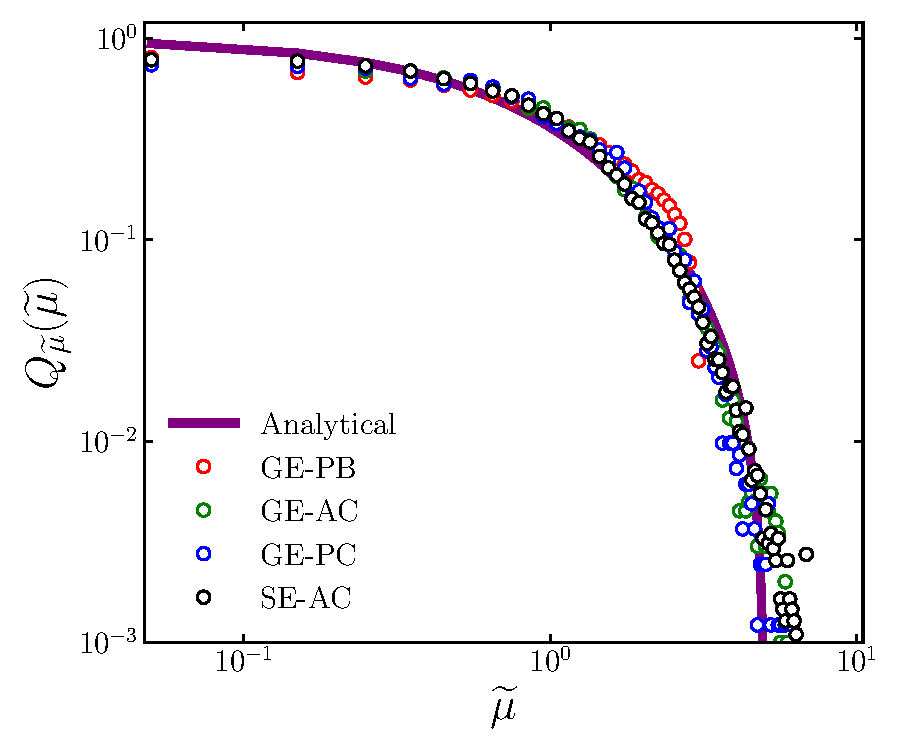
\includegraphics[width=0.8\linewidth]{chapters/chapter6/fig_4.pdf}
%     \caption{Scaled specific margin distributions $F(x)$ for multiple countries. While most countries (blue lines) follow the universal curve predicted by the RVM (black line), Ethiopia and Belarus (red lines) show significant deviations, suggesting potential electoral irregularities.}
%     \label{fig:anomalies}
% \end{figure}

\subsection{Case Studies: Electoral Anomalies}

Our analysis revealed two countries with pronounced deviations from the universal pattern: Ethiopia and Belarus. These deviations are significant enough to suggest potential irregularities in their electoral processes.

\subsubsection{The Ethiopia Case}

Ethiopia's 2010 election shows a striking deviation from the universal pattern, with the distribution of specific margins heavily skewed toward large values. This pattern indicates unusually large victory margins relative to turnout across the country's electoral units.

This statistical anomaly aligns with independent assessments of the 2010 Ethiopian election, which raised concerns about a restrictive political environment, uneven playing field, and potential irregularities in vote counting. The Ethiopia case demonstrates how the RVM can identify statistical signatures of electoral anomalies that correspond to documented concerns about electoral integrity.

\subsubsection{The Belarus Case}

Belarus similarly shows significant deviations from the universal pattern, with an overrepresentation of large specific margins. This statistical profile is consistent with concerns raised by international observers about Belarus's electoral processes, particularly regarding vote counting and tabulation.

The RVM's identification of statistical anomalies in both Ethiopia and Belarus demonstrates its value as an objective, quantitative tool for flagging potential concerns about electoral integrity. Importantly, these statistical indicators emerged purely from numerical analysis, without incorporating any qualitative assessments or contextual information about the countries' political systems.

\subsection{The RVM as a Statistical Baseline}

Beyond identifying potential irregularities, the RVM serves as a statistical baseline for understanding what "normal" electoral competition should look like. This baseline function has several valuable applications for election monitoring, historical analysis, cross-national comparison, and early warning of emerging concerns.

The RVM provides quantitative metrics to complement traditional monitoring approaches, allowing for standardized comparisons across different electoral systems. It can track the evolution of electoral competition over time, identifying shifts in statistical patterns that may indicate changes in the competitive environment. And it can serve as an early warning system, flagging unusual patterns that merit closer investigation by election observers and analysts.

\section{Limitations and Complementary Approaches}

While both the random nudge and the RVM provide valuable tools for addressing challenges to democratic processes, they have important limitations and should be viewed as complementary to other approaches rather than standalone solutions.

The random nudge approach cannot address structural causes of polarization such as economic inequality or institutional factors. Its effectiveness depends on implementation details and platform cooperation, and different cultural and political contexts may require different calibration. It may also be less effective against deliberate disinformation campaigns.

Similarly, the RVM diagnostic approach can identify statistical anomalies but cannot determine their causes. Some legitimate electoral systems may produce distributions that deviate from the universal pattern, and data quality issues can affect analysis results. Statistical signals must be interpreted in context alongside other evidence.

Both interventions are most effective when integrated with existing frameworks. The random nudge should complement media literacy programs, platform design improvements, and policy approaches to polarization. The RVM diagnostic tool should support, not replace, traditional election monitoring, legal frameworks, and institutional safeguards for electoral integrity.

\section{Implementation Pathways and Future Directions}

The translation of these theoretical tools into practical applications requires collaboration across multiple domains. For the random nudge, this includes conducting controlled trials to validate effectiveness and optimize parameters, forming partnerships with social media companies to implement and evaluate interventions, developing adaptive systems that learn and adjust intervention parameters based on observed effects, and incorporating user feedback and preferences into the design.

For the RVM diagnostic, implementation pathways include developing accessible software implementing RVM analysis for election observers and researchers, expanding data collection efforts to create more comprehensive and standardized electoral data, integrating statistical diagnostics into standard monitoring protocols, and training election officials and observers in statistical approaches to electoral integrity.

\section{From Research to Impact: The Path Forward}

Both applications—the random nudge for depolarization and the RVM for electoral diagnostics—represent promising pathways from fundamental research to real-world impact. Their development demonstrates how insights from statistical physics, complex systems, and computational social science can generate practical tools for strengthening democratic processes.

The ultimate success of these applications will depend on multidisciplinary collaboration, thoughtful implementation, and continuing refinement based on real-world experience. As we move forward, both approaches should be subject to rigorous validation, ethical scrutiny, and adaptation to diverse contexts.

In the concluding chapter, we will reflect on the broader implications of our research for understanding democratic processes and consider how the constructive use of randomness might inform other approaches to social system design and intervention. 
\newpage
\thispagestyle{empty}
\mbox{}

\chapter{Looking Forward: Randomness, Democracy, and Beyond}
\label{chap7}

As we conclude our exploration into the statistical mechanics of human collective behavior, this chapter synthesizes the key insights gained through our research, examines their broader implications, and outlines promising directions for future investigation. Throughout this thesis, we have demonstrated that randomness—often perceived as an impediment to understanding—emerges as both a powerful explanatory principle and a constructive force in complex social systems.

\section{The Unifying Thread: Randomness as Ally}

Our research consistently reveals the constructive power of randomness in complex social systems. In the context of opinion dynamics, we demonstrated how a simple "random nudge" intervention can effectively combat polarization on social networks without invasive monitoring of user opinions. This strategic application of randomness—introducing a probability $p$ for agents to interact uniformly rather than through homophilic preferences—successfully disrupts echo chambers and fosters depolarization even at small values ($p = 0.01$). The elegance of this solution lies in its non-intrusiveness; it requires no interpretation of user opinions, making it both privacy-preserving and practically implementable.

In the electoral domain, our Random Voting Model (RVM) reveals how the inherently stochastic nature of voting processes generates robust universal patterns across vastly different electoral systems, scales, and cultural contexts. By analytically deriving the scaled distribution of the margin-to-turnout ratio $F(x)$ where $x = \mu/\langle\mu\rangle$, we uncovered a remarkable universality across 32 democratic nations. This finding challenges conventional views that electoral outcomes are primarily determined by strategic campaigning or policy positions, suggesting instead that fundamental statistical processes play a dominant role in shaping electoral competition.

The power of randomness extends to practical applications as well. Our analysis demonstrates that deviations from the universal patterns predicted by the RVM can serve as effective statistical indicators of potential electoral irregularities, as evidenced in our analyses of elections in Ethiopia and Belarus. This approach transforms statistical noise into a valuable diagnostic tool for democratic integrity.

\section{Key Contributions and Their Implications}

\section{Methodological Contributions}

Our work significantly advances methodological approaches in computational social science. First, we demonstrate the critical importance of variable selection in uncovering universal patterns. While previous research focused on vote shares $q(\sigma)$ and turnouts $g(\tau)$, our identification of the margin-to-turnout ratio $\mu = M/T$ as the key variable revealed previously undetected universality. This emphasizes that appropriate variable transformation can be decisive in revealing underlying patterns in complex systems.

Second, our multi-scale analysis across different electoral hierarchies—from individual polling booths (~10² voters) to parliamentary constituencies (~10⁶ voters)—provides a robust validation framework for theoretical predictions. Particularly noteworthy is our discovery of scale invariance in Indian margin distributions, where $Q_M(M̃)$ shows a remarkable data collapse across different electoral scales. This methodological approach of cross-scale validation strengthens confidence in the RVM's theoretical foundations.

Third, we demonstrate the efficacy of minimalist models in capturing essential system properties. The parameter-free RVM, dependent only on turnout distributions and effective candidate numbers, successfully predicts not only the universal scaled specific margin distribution but also the distributions of winner and runner-up vote shares. This underscores the value of parsimonious modeling approaches that isolate fundamental mechanisms while abstaining from overfitting with excessive parameters.

\section{Theoretical Insights}

The RVM represents a significant advancement in understanding electoral competition. Our analytical derivations from order statistics establish a clear mathematical connection between random weight distributions and electoral outcomes. The model demonstrates that once turnout is "normalized out," a fundamental statistical process emerges that transcends specific electoral contexts.

The theoretical framework we developed extends beyond simply explaining observed universality. It provides analytical expressions for the distributions of winner votes, runner-up votes, and margins of victory as functions of turnout distribution. This allows us to predict how changes in voter participation patterns might affect electoral competitiveness—a valuable insight for democratic theory and practice.

Perhaps most profound is our demonstration that seemingly complex political phenomena can be governed by relatively simple statistical laws. This finding has implications beyond elections, suggesting that many social systems characterized by competition and collective choice may exhibit similar universal properties driven by underlying stochastic processes.

\section{Practical Impact}

Both the random nudge intervention and the RVM-based analytical framework demonstrate how theoretical insights can translate into practical applications. For online platforms struggling with polarization, our random nudge strategy offers a mathematically optimized approach that balances depolarization against potential radicalization. The power-law relationship we discovered—$p \cdot f^A = B$ where $p$ is the nudge probability, $f$ is the fraction of nudged population, and $A$ and $B$ are system-dependent constants—provides a concrete optimization framework for implementation.

In the electoral domain, the RVM serves as a powerful statistical baseline for competitive electoral outcomes. By comparing empirical distributions to model predictions, electoral authorities and independent observers can identify potential irregularities that warrant further investigation. This application is particularly valuable in contexts where traditional monitoring approaches face logistical or political challenges.

Both applications illustrate how statistical physics approaches can yield practical tools for addressing pressing societal challenges while respecting constraints such as user privacy and analytical tractability.

\section{Limitations and Open Questions}

Despite the robust findings presented in this thesis, several important limitations and open questions remain. Understanding these boundaries is crucial for both interpreting our results and guiding future research.

\section{Scope of Universality}

While we demonstrated remarkable universality in the scaled margin-to-turnout ratio across 32 countries, exceptions exist. Ethiopia and Belarus showed significant deviations that correlate with documented electoral irregularities. This raises important questions about the boundaries of the observed universality. Under what specific conditions might these universal patterns break down? How do factors such as electoral system design, party structure, or social inequality affect the statistical regularities? Further research across more diverse electoral contexts and longer time periods would help clarify these boundaries.

Additionally, the unique scale invariance we discovered in Indian margin distributions—absent in countries like the United States—suggests that certain electoral characteristics might produce distinctive statistical signatures. Understanding these distinctive patterns requires deeper investigation into the structural and procedural aspects of different electoral systems.

\section{Dynamic Processes}

Our current models treat elections primarily as independent statistical events, aggregating data across multiple elections to establish stable distributions. However, real political systems exhibit complex temporal dynamics, with feedback between consecutive electoral cycles. Understanding how universal patterns emerge and evolve over time remains an important challenge.

Future research should explore how electoral distributions change in response to major political realignments, institutional reforms, or demographic shifts. Temporal analyses could reveal whether the universal patterns we identified represent equilibrium states that systems naturally tend toward, or whether they require specific conditions to maintain.

\section{Strategic Interactions}

While the RVM successfully captures key electoral statistics without explicitly modeling strategic behavior, the role of coordinated action in shaping statistical patterns deserves further investigation. Political campaigns, parties, and voters all engage in strategic behavior that might influence the distributions we observe. 

An important question is whether strategic actors could, in principle, manipulate electoral processes to generate distributions that mimic the universal patterns we identified, thereby masking potential irregularities. Conversely, could knowledge of these statistical regularities enable more effective campaign strategies? These questions connect our statistical findings to broader issues of democratic theory and practice.

\section{Broader Implications for Social Science}

Our research contributes to a growing body of work applying physics principles to social phenomena, with several important implications for social science methodology and theory.

\section{The Value of Universal Perspectives}

The discovery of universal patterns in electoral competition demonstrates the value of searching for common principles that transcend specific contexts. Traditional social science approaches often emphasize institutional, historical, and cultural specificity—factors that are undoubtedly important. However, our findings suggest that beneath this complexity lie statistical regularities that operate across diverse contexts.

This universal perspective complements rather than contradicts contextual approaches. Understanding both the universal statistical processes and the specific factors that cause deviations provides a more complete picture of social phenomena. The value of this hybrid approach is evident in our anomaly detection application, where deviations from universal patterns signal contextual factors that warrant investigation.

\section{The Role of Scale}

Our multi-scale analysis of Indian elections reveals that certain statistical properties remain invariant across dramatically different scales of organization. This scale invariance suggests that similar underlying processes may operate across these different levels, challenging assumptions that different scales of social organization necessarily follow different principles.

The data collapse we observed in scaled margin distributions across polling booths, assembly constituencies, and parliamentary constituencies suggests that scaling relationships may be more common in social systems than previously recognized. This insight encourages researchers to look beyond single scales of analysis to identify properties that persist across organizational hierarchies.

\section{Intervention Design Principles}

The success of the random nudge in our opinion dynamics model suggests general principles for designing interventions in complex social systems. Rather than attempting to engineer specific outcomes through deterministic control, strategic introduction of randomness can effectively disrupt undesirable equilibria while preserving system autonomy.

This approach—combining minimal intervention with maximal impact—may be applicable to a wide range of social challenges where direct control is either impossible or undesirable. It exemplifies how understanding fundamental system dynamics can lead to elegant intervention strategies that work with rather than against natural system properties.

\section{Future Research Directions}

Our findings open several promising avenues for future research that could extend and deepen the insights presented in this thesis.

\section{Extension to Other Domains}

The principles we have developed may apply to other forms of collective decision-making and competitive processes. Market share competitions in business, citation distributions in science, attention allocation in media ecosystems, and resource distribution in organizational settings all involve competitive processes that might exhibit similar statistical regularities.

Testing these extensions would reveal the broader applicability of our theoretical framework. For example, does the market share ratio between leading companies follow similar universal distributions when scaled appropriately? Do scientific fields exhibit universal patterns in how citation advantages are distributed? These investigations could establish whether the statistical principles we identified are truly fundamental to competitive processes in general.

\section{Dynamic Models}

Developing theoretical frameworks that capture temporal evolution while preserving analytical tractability represents an important frontier. Future models could incorporate feedback mechanisms between consecutive electoral cycles, learning processes among voters and candidates, or evolutionary dynamics in party systems.

These dynamic extensions could address questions about system stability and change: Do electoral systems naturally evolve toward configurations that produce the universal distributions we observed? How do exogenous shocks affect these distributions, and how quickly do systems return to equilibrium? Understanding these temporal aspects would significantly advance our comprehension of democratic processes.

\section{Intervention Optimization}

The random nudge represents just one application of strategic randomness in social systems. Future research could explore other intervention designs based on similar principles. For example, could strategic randomization in news feed algorithms reduce both filter bubbles and user disengagement? Could random citizen assemblies enhance democratic representation while reducing polarization?

Optimization frameworks that balance multiple objectives—such as our approach to balancing depolarization against radicalization—could be developed for these new applications. This research direction connects theoretical insights to practical implementation challenges in ways that could significantly impact social system design.

\section{Technological and Societal Context}

Our work takes place against the backdrop of rapid technological change that is transforming both information systems and democratic processes, creating both challenges and opportunities for research application.

\section{Algorithmic Mediation}

As digital platforms increasingly mediate human interactions, understanding their effects on collective behavior becomes crucial. Our random nudge intervention directly addresses this context, offering a principled approach to modifying recommendation algorithms without compromising user privacy or platform functionality.

Future research should examine how different algorithmic architectures interact with the statistical processes we identified. Do certain recommendation systems naturally produce opinion distributions that resist polarization? Do social media platforms influence electoral statistics in detectable ways? These questions connect our theoretical work to urgent practical challenges in platform governance.

\section{Scale of Modern Democracy}

Democratic systems now operate at unprecedented scales, from local communities to national electorates numbering nearly a billion voters, as in India. The scale-invariant properties we discovered in Indian elections may be particularly relevant for understanding how democratic processes operate across these multiple levels.

Research on how statistical patterns propagate across scales could inform questions of democratic representation and governance. Do certain electoral system designs better preserve statistical regularity across scales? Does scale invariance correlate with perceived democratic legitimacy or citizen satisfaction? These questions connect our statistical findings to fundamental issues in democratic theory.

\section{Information Ecosystem Evolution}

The rapid evolution of information technologies creates constant flux in how citizens form opinions and make electoral choices. Adaptive intervention strategies that can evolve with changing technological landscapes will be essential for maintaining democratic health.

Our theoretical frameworks provide tools for analyzing these evolving systems, but must themselves adapt to changing conditions. Future research should explore how robust our statistical findings are to major technological shifts, and how intervention strategies might need to adjust in response to new information ecosystem dynamics.

\section{Ethical Considerations}

Our work raises important ethical questions about intervention in social systems that must be addressed as research moves toward practical application.

\section{Autonomy and Manipulation}

Any intervention in social systems raises questions about individual autonomy. The random nudge approach offers a partial answer by minimizing opinion monitoring and preserving user choice, but broader principles are needed for ethical intervention design.

Future research should explicitly address the ethical boundary between beneficial intervention and manipulation. When does structural modification of interaction patterns cross into problematic territory? What principles should guide the design and deployment of interventions? These questions require interdisciplinary engagement with ethics, law, and political philosophy alongside technical development.

\section{Democratic Legitimacy}

Statistical approaches to electoral analysis and intervention inevitably intersect with questions of democratic legitimacy. What gives researchers, platforms, or regulators the right to analyze or intervene in democratic processes? How can we ensure that such interventions serve the public interest rather than particular agendas?

These questions require transparent methodologies, public engagement, and institutional safeguards. Future research should explore how statistical tools like the RVM could be embedded in legitimate democratic institutions while preserving their analytical power and independence.

\section{Unintended Consequences}

All interventions in complex systems risk unintended consequences. For example, could random nudging strategies inadvertently advantage certain political viewpoints? Might statistical monitoring of elections create false positives that undermine legitimate results?

Designing safeguards and monitoring systems to detect and mitigate such effects is essential. This includes establishing clear baselines, implementing transparent methodologies, and developing mechanisms for corrective action when interventions produce unintended outcomes.

\section{The Road Ahead}

As we look to the future, several priorities emerge for advancing the research program initiated in this thesis.

\section{Interdisciplinary Collaboration}

The challenges we have addressed require collaboration across disciplines. Physicists contribute analytical tools and universality frameworks; political scientists provide institutional knowledge and normative perspectives; computer scientists develop implementation architectures; and practitioners ground theoretical insights in real-world constraints.

Future progress depends on strengthening these interdisciplinary connections. This includes developing shared vocabularies, creating joint research initiatives, and building educational programs that train researchers to work effectively across disciplinary boundaries.

\section{Real-World Testing}

Moving from theoretical insights to practical impact requires extensive real-world testing and validation. For the random nudge intervention, this might involve controlled trials with willing platform partners, measuring both immediate opinion dynamics and longer-term user satisfaction.

For electoral applications, validation could include retrospective analysis of elections with known irregularities, and prospective partnerships with electoral authorities to implement RVM-based monitoring systems. These real-world tests would not only validate our theoretical frameworks but also identify practical implementation challenges.

\section{Adaptive Frameworks}

Social systems evolve rapidly, requiring intervention strategies that can adapt to changing conditions. Future research should develop frameworks for continuous learning and adaptation, enabling interventions to remain effective as underlying systems change.

This might include automated parameter tuning for random nudge implementations, evolving analytical baselines for the RVM as electoral systems change, and flexible institutional arrangements that can incorporate new findings as they emerge.

\section{Final Reflections}

This thesis began with the observation that society represents one of the most fascinating complex systems in nature. Our research journey has demonstrated that this complexity need not preclude understanding or improvement. By applying the tools of statistical physics and embracing the constructive power of randomness, we have uncovered universal principles that transcend specific contexts and developed interventions that could strengthen democratic processes.

The universal patterns we discovered in electoral statistics—particularly the scaled distribution of margin-to-turnout ratios that holds across 32 countries—reveal a profound simplicity underlying apparent complexity. Similarly, our random nudge intervention demonstrates how a minimal perturbation to interaction rules can significantly alter system-level outcomes in opinion dynamics.

The path forward is challenging but promising. As information technologies continue to evolve and democratic systems face new pressures, the need for principled approaches to understanding and improving collective behavior will only grow. The frameworks we have developed provide a foundation for this ongoing work.

Our ultimate goal remains ambitious yet achievable: contributing to healthier information ecosystems and more robust democratic processes through principled analysis and thoughtful intervention. In an age of increasing complexity and polarization, the tools of statistical physics offer hope for finding order in chaos and building systems that serve human flourishing.

\section{Chapter Summary}

This concluding chapter has synthesized the key findings from our research on opinion dynamics and electoral statistics, highlighting how randomness serves as both an explanatory principle and an intervention strategy in complex social systems. We have detailed our methodological contributions, theoretical advances, and practical applications while acknowledging limitations and ethical considerations. The chapter outlines promising directions for future research that could extend and deepen our understanding of collective behavior across multiple domains. As technological and social changes continue to transform information ecosystems and democratic processes, the principles and approaches developed in this thesis offer valuable tools for building more resilient and equitable systems of collective decision-making. 
\newpage
\thispagestyle{empty}
\mbox{}

\bibliographystyle{unsrt}
\cleardoublepage \addcontentsline{toc}{chapter}{References}
\bibliography{ref}

\end{document}
